
%%%%%%%%%%%%%%%%%%%%%%%%%%%%%%%%%%%%%%%%%%%%%%%%%%%%%%%%%%%%%%%%%%%%%%%%
% Plantilla TFG/TFM
% Escuela Politécnica Superior de la Universidad de Alicante
% Realizado por: Jose Manuel Requena Plens
% Contacto: info@jmrplens.com / Telegram:@jmrplens
%%%%%%%%%%%%%%%%%%%%%%%%%%%%%%%%%%%%%%%%%%%%%%%%%%%%%%%%%%%%%%%%%%%%%%%%

%%%%%%%%%%%%%%%%%%%%%%%%
% FORMATO DEL DOCUMENTO
%%%%%%%%%%%%%%%%%%%%%%%%
% scrbook es la clase de documento
% Si se desea que no haya página en blanco entre capítulos añadir "openany" en los parámetros de la clase. Sino siempre los capítulos empezarán en página impar.
\documentclass[a4paper,11pt,titlepage]{scrbook}
\KOMAoption{toc}{bib,chapterentryfill} % Opciones del índice

% Paquete de formato para scrbook. Con marcas, linea-separador superior e inferior
\usepackage[automark,headsepline,footsepline]{scrlayer-scrpage}
\clearpairofpagestyles		% Borra los estilos por defecto
%%
% Formato y contenido de la información de cabecera y pie de página
%%
% Información de capítulo en cabecera e interno
\ihead{{\color{gray30}\scshape\small\headmark}}	
% Número de página en cabecera y externo
\ohead{\normalfont\pagemark} 
% Número de página en pie de página y externo. Sólo en páginas sin cabecera
\ofoot[\normalfont\pagemark]{}
%% 		
% Edición del contenido de las distintas partes de la cabecera
%%
\renewcommand{\chaptermark}[1]{\markboth{#1}{}} % Capítulo (Solo texto)
\renewcommand{\sectionmark}[1]{\markright{\thesection. #1}} % Sección (Número y texto)
\setkomafont{pagenumber}{} % Número de página (Sin nada añadido)

% Añade al índice y numera hasta la profundidad 4.
% 1:section,2:subsection,3:subsubsection,4:paragraph
\setcounter{tocdepth}{4}
\setcounter{secnumdepth}{4}
% Muestra una regla para comprobar el formato de las páginas
%\usepackage[type=upperleft,showframe,marklength=8mm]{fgruler}
% MÁRGENES DE LAS PÁGINAS
\usepackage[
  inner	=	3.0cm, % Margen interior
  outer	=	2.5cm, % Margen exterior
  top	=	2.5cm, % Margen superior
  bottom=	2.5cm, % Margen inferior
  includeheadfoot, % Incluye cabecera y pie de página en los márgenes
]{geometry}
% Valor de interlineado
\renewcommand{\baselinestretch}{1.0} % 1 línea de interlineado


%%%%%%%%%%%%%%%%%%%%%%%%
% BIBLIOGRAFÍA
%%%%%%%%%%%%%%%%%%%%%%%%
\usepackage{apacite} % NORMA APA
\usepackage{natbib}
\usepackage{breakcites}

%%%%%%%%%%%%%%%%%%%%%%%%
% DOCUMENTO EN ESPAÑOL
%%%%%%%%%%%%%%%%%%%%%%%%
\usepackage{polyglossia}
\setdefaultlanguage{spanish}

\usepackage{longtable,booktabs,array}
\newcolumntype{L}[1]{>{\raggedright\let\newline\\\arraybackslash\hspace{0pt}}m{#1}}
\newcolumntype{C}[1]{>{\centering\let\newline\\\arraybackslash\hspace{0pt}}m{#1}}
\newcolumntype{R}[1]{>{\raggedleft\let\newline\\\arraybackslash\hspace{0pt}}m{#1}}

%%%%%%%%%%%%%%%%%%%%%%%% 
% COLORES
%%%%%%%%%%%%%%%%%%%%%%%% 
% Biblioteca de colores
\usepackage{color}
\usepackage[dvipsnames]{xcolor}
% Otros colores definidos por el usuario
\definecolor{gray97}{gray}{.97}
\definecolor{gray75}{gray}{.75}
\definecolor{gray45}{gray}{.45}
\definecolor{gray30}{gray}{.30}
\definecolor{negro}{RGB}{0,0,0}
\definecolor{blanco}{RGB}{255,255,255}
\definecolor{dkgreen}{rgb}{0,.6,0}
\definecolor{dkblue}{rgb}{0,0,.6}
\definecolor{dkyellow}{cmyk}{0,0,.8,.3}
\definecolor{gray}{rgb}{0.5,0.5,0.5}
\definecolor{mauve}{rgb}{0.58,0,0.82}
\definecolor{deepblue}{rgb}{0,0,0.5}
\definecolor{deepred}{rgb}{0.6,0,0}
\definecolor{deepgreen}{rgb}{0,0.5,0}
\definecolor{MyDarkGreen}{rgb}{0.0,0.4,0.0}
\definecolor{bluekeywords}{rgb}{0.13,0.13,1}
\definecolor{greencomments}{rgb}{0,0.5,0}
\definecolor{redstrings}{rgb}{0.9,0,0}



%%%%%%%%%%%%%%%%%%%%%%%% 
% FIGURAS, TABLAS, ETC 
%%%%%%%%%%%%%%%%%%%%%%%% 
\usepackage{subcaption} % Para poder realizar subfiguras
\usepackage{caption} % Para aumentar las opciones de diseño
% Nombres de figuras, tablas, etc, en negrita la numeración, todo con letra small
\captionsetup{labelfont={bf,small},textfont=small}
% Paquete para modificar los espacios arriba y abajo de una figura o tabla
\usepackage{setspace}
% Define el espacio tanto arriba como abajo de las figuras, tablas
\setlength{\intextsep}{5mm}
% Para ajustar tamaños de texto de toda una tabla o grafica
% Uso: {\scalefont{0.8} \begin{...} \end{...} }
\usepackage{scalefnt}
% Redefine las tablas y figuras para eliminar el '.' entre la numeración y el texto
\renewcommand*{\figureformat}{\figurename~\thefigure}
\renewcommand*{\tableformat}{\tablename~\thetable}

%%%%%%%%%%%%%%%%%%%%%%%% 
% TEXTO
%%%%%%%%%%%%%%%%%%%%%%%%
% Paquete para poder modificar las fuente de texto
\usepackage{xltxtra}
% Cualquier tamaño de texto. Uso: {\fontsize{100pt}{120pt}\selectfont tutexto}
\usepackage{anyfontsize}
% Para modificar parametros del texto.
\usepackage{setspace}
% Paquete para posicionar bloques de texto
\usepackage{textpos}
% Paquete para realizar cajas de texto. 
% Uso: \begin{mdframed}[linecolor=red!100!black] tutexto \end{mdframed}
\usepackage{framed,mdframed}
% Para subrayar. Uso: \hlc[tucolor]{tutexto}
\newcommand{\hlc}[2][yellow]{ {\sethlcolor{#1} \hl{#2}} }

% Para introducir url's con formato. Uso: \url{http://www.google.es}
\usepackage{url}
% Amplia muchas funciones graficas de latex
\usepackage{graphicx}
% Paquete que añade el hipervinculo en referencias dentro del documento, indice, etc
% Se define sin bordes alrededor. Uso: \ref{tulabel}
\usepackage[pdfborder={000}]{hyperref}
\usepackage{float}
\usepackage{verbatim}
% Paquete para condicionales avanzados
\usepackage{xstring,xifthen}
% Paquete para realizar calculos en el código
\usepackage{calc}
% Para rotar tablas o figuras o su contenido
\usepackage{rotating} 
\usepackage{tikz,tikzpagenodes}

% PAQUETES PUESTOS POR MÍ
\usepackage{enumitem}
\usepackage{booktabs}
\usepackage{array}


\usetikzlibrary{tikzmark,calc,shapes.geometric,arrows,backgrounds,shadings,shapes.arrows,shapes.symbols,shadows,positioning,fit,automata,patterns,intersections}

%%%%%%%%%%%%%%%%%%%%%%%% 
% GLOSARIOS
%%%%%%%%%%%%%%%%%%%%%%%%
\usepackage[acronym,nonumberlist,toc]{glossaries}
\usepackage{glossary-superragged}
\newglossarystyle{modsuper}{%
  \setglossarystyle{super}%
  \renewcommand{\glsgroupskip}{}
}
\renewcommand{\glsnamefont}[1]{\textbf{#1}}


%%%%%%%%%%%%%%%%%%%%%%%% 
% COMANDOS AÑADIDOS
%%%%%%%%%%%%%%%%%%%%%%%%
% Para mostrar la fecha actual (mes año) con \Hoy
\newcommand{\MES}{%
  \ifcase\month% 0
    \or Enero% 1
    \or Febrero% 2
    \or Marzo% 3
    \or Abril% 4
    \or Mayo% 5
    \or Junio% 6
    \or Julio% 7
    \or Agosto% 8
    \or Septiembre% 9
    \or Octubre% 10
    \or Noviembre% 11
    \or Diciembre% 12
  \fi}
\newcommand{\ANYO}{\number\year}
\newcommand{\Hoy}{\MES\ \ANYO}

%%%%%%%%%%%%%%%%%%%%%%%% 
% MATEMÁTICAS
%%%%%%%%%%%%%%%%%%%%%%%%
\usepackage{mathtools,amsthm,amsfonts,amssymb,bm,mathrsfs,nicefrac,upgreek,bigints} 
% Comando para añadir información de variables a las ecuaciones
% Uso: \begin{condiciones}[donde:] ....... \end{condiciones}
\newenvironment{condiciones}[1][2]
  {%
   #1\tabularx{\textwidth-\widthof{#1}}[t]{
     >{$}l<{$} @{}>{${}}c<{{}$}@{} >{\raggedright\arraybackslash}X
   }%
  }
  {\endtabularx\\[\belowdisplayskip]}

%%%%%
% DEFINICION DE CONCEPTOS
%%%%
% Uso ejemplo: \begin{ejemplo} tucontenido \end{ejemplo} 
\newtheorem{teorema}{Teorema}[chapter]
\newtheorem{ejemplo}{Ejemplo}[chapter]
\newtheorem{definicion}{Definición}[chapter]



% Título y subtítulo
\newcommand{\titulo}{Aplicación de AR/VR en edificios en construcción}
% Datos del autor
\newcommand{\miNombre}{Mario Giménez López-Torres }
\newcommand{\miEmail}{mgl126@alu.ua.es}
% Datos del tutor/es
\newcommand{\miTutor}{Francisco Gómez Donoso}
\newcommand{\miTutorB}{Miguel A. Cazorla Quevedo}
\newcommand{\departamentoTutor}{\href{https://web.ua.es/es/dccia/}{Departamento de Ciencia de la Computación e Inteligencia Artificial} }
\newcommand{\departamentoTutorB}{Departamento de Ciencia de la Computación e Inteligencia Artificial}
% Datos de la facultad y universidad
\newcommand{\miFacultad}{Escuela Politécnica Superior}
\newcommand{\miFacultadCorto}{EPS UA}
\newcommand{\miUniversidad}{\protect{Universidad de Alicante}}
\newcommand{\miUbicacion}{Alicante}

% Información añadida a las propiedades del archivo PDF.
\hypersetup{
pdfauthor = {\miNombre~(\miEmail)},
pdftitle = {\titulo},
}

% INDICA TU TITULACIÓN
% ID	GRADO -------------------------------------------------
% 1		Ingeniería en Imagen y Sonido en Telecomunicación
% 2		Ingeniería Civil
% 3		Ingeniería Química
% 4		Ingeniería Informática
% 5		Ingeniería Multimedia
% 6		Arquitectura Técnica
% 7		Arquitectura
% 8		Robótica
% %		%%%%%%%%%%%%
% ID	MÁSTER ------------------------------------------------
% A		Telecomunicación
% B		Caminos, Canales y Puertos
% C		Gestión en la Edificación
% D		Desarrollo Web
% E		Materiales, Agua, Terreno
% F		Informática
% G 	Automática y Robótica
% H		Prevención de riesgos laborales
% I		Gestión Sostenible Agua
% J		Desarrollo Aplicaciones Móviles
% K		Ingeniería Química
% L		Ciberseguridad
% M		Biomédica

\def\IDtitulo{5} % INTRODUCE LA ID DE TU TITULACIÓN				

% Configuración automática según el identificador elegido
\input{include/configuraciontitulacion} 


%%
% Archivo de acrónimos
%%
\makeglossaries % Genera la base de datos de acrónimos
%%%%%%%%%%%%%%%%%%%%%%%%%%%%%%%%%%%%%%%%%%%%%%%%%%%%%%%%%%%%%%%%%%%%%%%%
% Plantilla TFG/TFM
% Escuela Politécnica Superior de la Universidad de Alicante
% Realizado por: Jose Manuel Requena Plens
% Contacto: info@jmrplens.com / Telegram:@jmrplens
%%%%%%%%%%%%%%%%%%%%%%%%%%%%%%%%%%%%%%%%%%%%%%%%%%%%%%%%%%%%%%%%%%%%%%%%

% Lista de acrónimos (se ordenan por orden alfabético automáticamente)

% La forma de definir un acrónimo es la siguiente:
% \newacronym{id}{siglas}{descripción}
% Donde:
% 	'id' es como vas a llamarlo desde el documento.
%	'siglas' son las siglas del acrónimo.
%	'descripción' es el texto que representan las siglas.
%
% Para usarlo en el documento tienes 4 formas:
% \gls{id} - Añade el acrónimo en su forma larga y con las siglas si es la primera vez que se utiliza, el resto de veces solo añade las siglas. (No utilices este en títulos de capítulos o secciones).
% \glsentryshort{id} - Añade solo las siglas de la id
% \glsentrylong{id} - Añade solo la descripción de la id
% \glsentryfull{id} - Añade tanto  la descripción como las siglas

\newacronym{3dgs}{3DGS}{3D Gaussian Splatting} % AÑADIDO
\newacronym{3dof}{3DoF}{3 Grados de Libertad} % AÑADIDO
\newacronym{6dof}{6DoF}{6 Grados de Libertad} % AÑADIDO
\newacronym{abp}{ABP}{Aprendizaje Basado en Proyectos} % AÑADIDO
\newacronym{apis}{APIs}{Application Programming Interfaces} % AÑADIDO
\newacronym{ar}{AR}{Realidad Aumentada} % AÑADIDO
\newacronym{b2b}{B2B}{Business-to-Business} % AÑADIDO
\newacronym{bcf}{BCF}{BIM Collaboration Format} % AÑADIDO
\newacronym{bim}{BIM}{Building Information Modeling} % AÑADIDO
\newacronym{cac}{CAC}{Customer Acquisition Cost} % AÑADIDO
\newacronym{cii}{CII}{Construction Industry Institute} % AÑADIDO
\newacronym{cobie}{COBie}{Construction Operations Building Information Exchange} % AÑADIDO
\newacronym{cpu}{CPU}{Unidad de Central de Procesamiento} % AÑADIDO
\newacronym{dafo}{DAFO}{Debilidades, Amenazas, Fortalezas y Oportunidades}% AÑADIDO
\newacronym{fbx}{FBX}{Filmbox} % AÑADIDO
\newacronym{fps}{FPS}{Fotogramas por Segundo} % AÑADIDO
\newacronym{gdpr}{GDPR}{General Data Protection Regulation} % AÑADIDO
\newacronym{gps}{GPS}{Global Positioning System} % AÑADIDO
\newacronym{gpu}{GPU}{Unidad de Procesamiento Gráfico} % AÑADIDO
\newacronym{gui}{GUI}{Interfaz Gráfica de Usuario} % AÑADIDO
\newacronym{ia}{IA}{Inteligencia Artificial} % AÑADIDO
\newacronym{ide}{IDE}{Entorno de Desarrollo Integrado} % AÑADIDO
\newacronym{ifc}{IFC}{Industry Foundation Classes} % AÑADIDO
\newacronym{iot}{IoT}{Internet of Things} % AÑADIDO
\newacronym{lcd}{LCD}{Liquid Crystal Display} % AÑADIDO
\newacronym{lod}{LOD}{Nivel de Desarrollo} % AÑADIDO
\newacronym{ltv}{LTV}{Lifetime Value} % AÑADIDO
\newacronym{mau}{MAU}{Usuarios Activos Mensuales} % AÑADIDO
\newacronym{m2p}{M2P}{Latencia de fotones a movimiento} % AÑADIDO
\newacronym{mep}{MEP}{Mechanical, Electrical, and Plumbing} % AÑADIDO
\newacronym{moscow}{MoSCoW}{Must have, Should have, Could have, Won't have} % AÑADIDO
\newacronym{mvp}{MVP}{Producto Mínimo Viable} % AÑADIDO
\newacronym{nerf}{NeRF}{Neural Radiance Fields} % AÑADIDO
\newacronym{nps}{NPS}{Net Promoter Score} % AÑADIDO
\newacronym{pc}{PC}{Ordenador Personal} % AÑADIDO
\newacronym{pdf}{PDF}{Portable Document Format} % AÑADIDO
\newacronym{peou}{PEOU}{Facilidad de Uso Percibida} % AÑADIDO
\newacronym{pu}{PU}{Utilidad Percibida} % AÑADIDO
\newacronym{ram}{RAM}{Random Access Memory} % AÑADIDO
\newacronym{roi}{ROI}{Retorno de la Inversión} % AÑADIDO
\newacronym{saas}{SaaS}{Software as a Service} % AÑADIDO
\newacronym{sdks}{SDKs}{Software Development Kits} % AÑADIDO
\newacronym{slam}{SLAM}{Simultaneous Localization and Mapping} % AÑADIDO
\newacronym{soc}{SoC}{System on a Chip} % AÑADIDO
\newacronym{sor}{SOR}{Filtrado Estadístico de Ruido} % AÑADIDO
\newacronym{tam}{TAM}{Modelo de Aceptación Tecnológica}
\newacronym{tfg}{TFG}{Trabajo Fin de Grado} % AÑADIDO
\newacronym{ui}{UI}{Interfaz de Usuario} % AÑADIDO
\newacronym{vr}{VR}{Realidad Virtual} % AÑADIDO
\newacronym{xr}{XR}{Realidad Extendida} % AÑADIDO
 % Archivo que contiene los acrónimos

\begin{document}

% Números romanos hasta el mainmatter.
\frontmatter

% PORTADA
\input{include/portada/portada_color} % Portada Color
\input{include/portada/portada_bn} % Portada B/N

%%%%% PREAMBULO
% Incluye el .tex que contiene el preámbulo, agradecimientos y dedicatorias.

\chapter*{Preámbulo}
\thispagestyle{empty}
    La industria de la construcción de edificios consiste en un proceso que requiere la comunicación de diferentes agentes involucrados en un proyecto, desde el momento en el que se diseñan los planos hasta que el edificio está listo. Arquitectos, ingenieros, contratistas y clientes deben compartir una visión común del edificio que, tradicionalmente, se ha transmitido mediante planos en papel o bidimensionales, junto con maquetas o imágenes estáticas que no siempre facilitan una compresión espacial completa del proyecto.

    Esta desconexión entre la representación técnica y la percepción real genera problemas recurrentes en esta industria: malinterpretaciones de diseño, errores no detectados hasta fases avanzadas de obra, dificultades para validar decisiones en la construcción y barreras en la comunicación con clientes que no tienen conocimientos técnicos. Las metodologías actuales, aunque rigurosas, no explotan el potencial de las tecnologías de realidad inmersiva, las cuales podrían transformar cómo se visualiza y verifica un proyecto arquitectónico.

    Este trabajo propone una solución con el desarrollo de una aplicación que integre Realidad Virtual y/o Realidad Aumentada en el flujo de trabajo de construcción, permitiendo visualizar modelos \gls{bim} directamente en éstas. La investigación previa identificará las necesidades específicas del sector y evaluará qué tecnologías y enfoques resultan más efectivos para cada tipo de tarea.

    El resultado será una aplicación multiplataforma que combine visualización 3D en tiempo real integración con modelos BIM existentes y funcionalidades adaptadas a casos de uso concretos como inspecciones de obra, formación de seguridad o presentaciones a clientes, respaldada por una arquitectura técnica robusta capaz de gestionar grandes volúmenes de información geométrica.


\chapter*{Motivación, justificación y objetivo general}

    Hace alrededor de 2 años, compré mis primeras gafas de realidad virtual, las Meta Quest 2, y es algo de lo que no me arrepiento para nada haber obtenido, ya que es una experiencia que opino que todo el mundo debería experimentar al menos una vez, la inmersión que te da pareciendo que estás en otro mundo da otra sensación de control, sobre todo en los videojuegos.
    Mientras reflexionaba sobre qué tema escogería para mi \gls{tfg}, llegué a la conclusión de que la industria de la realidad virtual o aumentada tiene mucho futuro y margen de mejora, las gafas que tengo, aunque no sean las más recientes, siguen siendo modernas, pero tienen problemas que necesitan arreglo, como el sobrecalentamiento, la potencia o su pesado diseño. Problemas que el siguiente modelo soluciona ligeramente pero no al completo.
    Por razones como esta pienso que los campo de la \gls{ar} y \gls{vr} son de las más interesantes para estudiar ya que, al igual que la \gls{ia}, en un futuro tendrán mucha más relevancia en el ámbito lúdico y laboral, siendo en este caso la construcción de edificios, una de las más imprescindibles en la sociedad. En un tiempo se perfeccionarán estos dispositivos de realidad virtual con el objetivo de que sean más accesibles, versátiles y normalizados.
    Aunque en la formación obtenida actualmente esta industria no es algo en lo que haya llegado a profundizar mucho, me ha ayudado a asentar las bases de la programación, gestión de proyectos y diseño de interfaces que me ayudarán para realizar el proyecto. Este TFG lo utilizaré como entrada para especializarme en este campo.

\cleardoublepage %salta a nueva página impar
\chapter*{Agradecimientos}

\thispagestyle{empty}
\vspace{1cm}

    Con este trabajo me gustaría agradecer a los familiares, empezando por mi madre y mi padrastro por el apoyo incondicional que me han dado por todas mis difíciles etapas de estudio, ayudándome a salir adelante y levantándome cada vez que lo necesitaba para seguir esforzándome.
    Además también quiero dar las gracias a mi hermano, que me ha echado una mano con las asignaturas que he tenido dificultad durante la carrera y me ha enseñado que  llegar hasta aquí siempre ha sido posible.
    Por otro lado también quisiera mostrar agradecimiento a mis amigos, sobre todo a los que se han quedado conmigo hasta el final de esta dura carrera, por escucharme en cada momento y crear buenos momentos, los cuales hasta el día de hoy siguen siendo dignos de recordar.
    Por último, quiero agradecer también a mis compañeros del grupo de \gls{abp}, por haber hecho de ese proyecto incluso de esa magnitud un proceso ameno y en el que me lo he llegado a pasar bien.

    

\cleardoublepage %salta a nueva página impar

\begin{quote}
``\textit{Listen, it's the times when you're scared or worried that you should deal with smiling!}''

\raggedleft --- All Might (Kenta Miyake)
\end{quote}

\begin{quote}
``\textit{I will fight for my future! I will fight alongside the future that everyone created for me! It’s not for anyone else’s sake but my own!}''

\raggedleft --- Hajime Hinata (Johnny Yong)
\end{quote}


%\cleardoublepage %salta a nueva página impar
% Aquí va la cita célebre si la hubiese. Si no, comentar la(s) linea(s) siguientes
%\chapter*{}
%\setlength{\leftmargin}{0.5\textwidth}
%\setlength{\parsep}{0cm}
%\addtolength{\topsep}{0.5cm}
%\begin{flushright}
%\small\em{
%Si consigo ver más lejos\\
%es porque he conseguido auparme\\ 
%a hombros de gigantes
%}
%\end{flushright}
%\begin{flushright}
%\small{
%Isaac Newton.
%}
%\end{flushright}
%\cleardoublepage %salta a nueva página impar
 

% Incluye después del archivo anterior el indice y lista de figuras, tablas y códigos.
\tableofcontents	% Índice
\listoffigures		% Índice de figuras
\listoftables		% Índice de tablas

% Inicia la numeración habitual.
\mainmatter

%%%%
% CONTENIDO. CAPÍTULOS DEL TRABAJO - Añade o elimina según tus necesidades
%%%%
\chapter{Introducción}
    El desarrollo de proyectos arquitectónicos, concretamente en el aspecto de la visualización, ha evolucionado de manera constante desde los primeros planos dibujados a mano hasta los modelos digitales tridimensionales de hoy en día. Durante décadas, arquitectos e ingenieros han confiado en el dibujo técnico de representaciones bidimensionales, planos, secciones y alzados para explicar sus diseños a constructores, inversores y clientes. Sin embargo, esta forma de comunicación tiene limitaciones, ya que requiere de conocimientos técnicos específicos para su correcta interpretación y hace difícil la comprensión espacial completa del proyecto, especialmente para personas sin formación en el sector.

    Con la aparición de la metodología BIM (Building Information Modeling), esta industria dio un salto considerable al juntar geometría tridimensional con información técnica detallada de cada elemento de la construcción. No obstante, incluso los modelos BIM más avanzados se visualizan habitualmente en pantallas convencionales, lo que mantiene esa dificultad perceptiva entre el diseño digital y la experiencia física del espacio construido. Esto hace que se generen problemas de manera recurrente: malinterpretaciones o dificultades para validar decisiones durante la fase de ejecución y barreras comunicativas con clientes.

    De manera paralela, en la última década, las tecnologías de Realidad Aumentada (AR), y Realidad Virtual (VR) se han desarrollado o perfeccionado lo suficiente para que sean aplicables en estos sectores de manera profesional. Dispositivos como Microsoft HoloLens, Meta Quest o smartphones de gama media ya poseen capacidades de seguimiento espacial, renderizado en tiempo real y experiencias inmersivas a costes cada vez más asequibles. Estas tecnologías permiten superponer información digital sobre el entorno físico real (AR) o sumergir completamente al usuario en un espacio virtual (VR), abriendo posibilidades para el sector de la construcción.

    Actualmente, diversas empresas y estudios de arquitectura han comenzado a experimentar con soluciones AR/VR de forma aislada, por ejemplo, visualizar el interior de un piso para su compra. Sin embargo, la mayoría son herramientas propietarias, es decir, carecen de integración fluida con flujos de trabajo BIM existentes o están diseñadas para casos de uso muy específicos. Por lo tanto, existe la posibilidad de desarrollar una aplicación integral que aproveche estas tecnologías inmersivas y satisfaga las necesidades reales de los profesionales del sector.

    El objetivo de este trabajo es diseñar y desarrollar una aplicación basada en Realidad Virtual y/o Realidad Aumentada orientada específicamente al ámbito de la construcción de edificios. El objetivo de este proyecto permitirá visualizar modelos BIM directamente sobre el emplazamiento real mediante dispositivos AR, facilitando la inspección de obra, la detección temprana de errores entre proyecto y ejecución, y la comunicación efectiva entre los equipos de las distintas fases. Asimismo, ofrecerá experiencias inmersivas en VR para recorrer virtualmente el proyecto antes de su construcción, evaluar su diseño, realizar formaciones en procedimientos de seguridad y presentar propuestas a clientes de manera comprensible e impactantes.

    Este proyecto se estructura en varias fases. En primer lugar, se llevará a cabo un análisis exhaustivo del estado del arte en tecnologías en AR/VR aplicadas a la construcción, identificando las soluciones existentes, sus limitaciones y las necesidades no cubiertas. Después, se definirá la arquitectura del sistema, seleccionando las plataformas de desarrollo más adecuadas, estableciendo la integración con formatos BIM estándar (como IFC o Revit) y diseñando la interfaz de usuario para que su interacción sea intuitiva con entornos inmersivos. La fase de desarrollo incluirá la implementación de funcionalidades clave como la medición métrica, la generación de informes y la visualización de datos técnicos. Finalmente, se realizarán pruebas en edificios reales para validar la usabilidad y efectividad de la solución.

    Las tecnologías inmersivas eliminan la abstracción que suponen los planos tradicionales y acercan el diseño digital a la percepción humana del espacio real. Este trabajo busca contribuir a estas tecnologías, proporcionando una herramienta práctica que mejore la eficiencia, reduzca errores y potencie la colaboración en los proyectos de construcción.

    El resto de este documento está estructurado de la siguiente manera:
    
    En primer lugar, en el Capítulo 2 se presenta el estudio de viabilidad, donde se analiza el contexto y mercado del proyecto mediante herramientas: una matriz DAFO (Cuadro~\ref{tab:dafo}), un modelo Lean Canvas (Cuadro~\ref{tab:lean-canvas}) y un análisis de riesgos (Cuadro~\ref{tab:riesgos}).
    
    Posteriormente, el Capítulo 3 define los objetivos principales y específicos, incluyendo la planificación temporal y una revisión exhaustiva del estado del arte de las tecnologías inmersivas y BIM. 
    
    En el Capítulo 4 se expone la metodología de trabajo adoptada para el proyecto, basada en Kanban, así como las herramientas utilizadas para su gestión.
    
    Por otro lado, el Capítulo 5 entra en detalle sobre el desarrollo técnico de la aplicación, describiendo la implementación de los diferentes sistemas como la selección de elementos BIM.
    
    Finalmente, los Capítulos 6 y 7 recogen, respectivamente, los resultados obtenidos tras las pruebas de la aplicación y las conclusiones finales a partir de la realización de este trabajo.


	% Plantilla: Se muestran contenidos
\chapter{Estudio de viabilidad}
    Para poder dar inicio a este proyecto es necesario evaluar previamente sus posibilidades reales de éxito. Esta etapa no se centra solo en su desarrollo inicial como TFG, sino enfocado también a una potencial evolución futura más allá del ámbito académico.

   Con el objetivo de saber si realmente merece la pena invertir esfuerzos y recursos en esta aplicación, hay que examinar el proyecto desde distintas perspectivas, identificando tanto los factores que juegan a favor como aquellos obstáculos que podrían dificultar su progreso o limitar su impacto.

   Hay que tener en cuenta que este proyecto no se trata de inventar algo completamente nuevo. Ya existen herramientas en el mercado que abordan parcialmente problemas similares, pero en este caso está el propósito de mejorar esas propuestas actuales y adaptarse mejor a las necesidades específicas de los profesionales del sector.

   A continuación, se aplicarán distintas metodologías de análisis que permitirán obtener una visión completa de la situación. De esta forma, se podrá determinar la solidez del proyecto.

  
\section{Análisis DAFO} 

    El análisis DAFO (Debilidades, Amenazas, Fortalezas y Oportunidades), también conocido por sus siglas en inglés como análisis SWOT (Strengths, Weaknesses, Opportunities, Threaths), es una herramienta de diagnóstico ampliamente utilizada en la gestión de proyectos y la planificación empresarial\footnote{\cite{weihrich1982daws}}. Sirve para evaluar la situación actual de un producto o servicio, identificando tanto los factores internos como externos que pueden influir en su desarrollo y éxito.

    Esta metodología tiene 4 dimensiones principales, al ser una matriz 2x2. La primera examina los factores internos del proyecto, sobre los que se tiene control directo, clasificándolos como fortalezas (ventajas competitivas) y debilidades (limitaciones o carencias). Por otro lado, se analizan los factores externos, sobre los que no se ejerce control pero que afectan al proyecto, siendo oportunidades (circunstacias favorables aprovechables) y amenazas (riesgos que pueden comprometer el progreso).

    El principal objetivo de este análisis es proporcionar una visión para tomar decisiones que potencien las fortalezas, mitiguen las debilidades, exploten las oportunidades y anticipen las amenazas. Dado que en este proyecto académico convergen distintos factores técnicos, económicos y sociales, resulta conveniente.
\begin{itemize}
\item \textbf{Fortalezas}: Una fortaleza destacable es la actualidad y relevancia del problema que se pretende resolver. Las tecnologías inmersivas tienen cada vez más presencia en el día a día, abriendo muchas posibilidades de innovación en el futuro. Por otro lado, la industria de la construcción es imprescindible e indispensable para la práctica totalidad de las civilizaciones, por lo que es un proyecto muy versátil para muchas empresas.

En segundo lugar, este proyecto es desarrollado por una persona, lo que optimiza la toma de decisiones, ya que, a excepción del tutor, no se necesita mucha más validación. Además, no requiere coordinar el progreso de este proyecto con otras personas. Los objetivos serán más claros ya que el producto tendrá el límite de capacidad de trabajo de una sola persona, centrándose en desarrollar los aspectos más imprescindibles.

Por último, el autor ya tiene experiencia en el uso de dispositivos de realidad virtual/aumentada, aunque sin tener conocimientos de todas las posibilidades que tiene, ya está familiarizado con las interfaces, controles y funciones básicas de éstos.

\item \textbf{Debilidades}: A pesar de tener experiencia en el uso práctico de estas tecnologías, una de las debilidades más destacables es la falta de conocimiento en el campo de desarrollo específicamente, como se ha comentado en la motivación, uno de los objetivos de este TFG es introducirse en la industria de aplicaciones AR/VR y ver si es algo en lo que especializarse, por lo que aspectos como el seguimiento espacial, optimización para renderizado en tiempo real y diseño de interfaces tridimensionales difieren del desarrollo software convencional, lo que implica invertir más tiempo para familiarizarse con nuevas tecnologías de desarrollo.

Otra debilidad es la falta de recursos financieros. Aunque existen a disposición herramientas de desarrollo gratuitas o con licencias educativas, ciertos aspectos como acceder a librerías premium o assets podría requerir inversión económica. Esta limitación condiciona las decisiones tecnológicas y puede afectar al alcance funcional del producto final.

Después estarían las obligaciones académicas simultáneas, al estar cursando el último año de Ingeniería Multimedia a tiempo completo, esto restará tiempo que se podría invertir en este proyecto, ralentizando el progreso y dificultando el mantener la concentración en aspectos complejos del proyecto.

Finalmente, la limitación de alcance inherente a un TFG impide desarrollar un producto completamente funcional y comercializable. El tiempo disponible obligará a priorizar funcionalidades imprescindibles y a implementar prototipos o demostraciones de concepto en lugar de sistemas robustos listos para producción y venta, afectando la viabilidad real de esta aplicación.

\item \textbf{Oportunidades}: Este proyecto presenta un contexto actual que da múltiples oportunidades favorables para su aplicación práctica. La creciente adopción de metodologías BIM en el sector de la construcción, impulsada incluso por normativas en diversos países\footnote{~\cite{ukcabinet2016strategy, eubim2017handbook, fomento2015comision}}, genera una base de datos de modelos 3D estructurados que pueden servir como información para alimentar la aplicación.

Por otro lado, la evolución acelerada de dispositivos AR/VR representa otra oportunidad considerable. Los smartphones actuales incorporan capacidades AR nativas, las gafas de realidad mixta están mejorando rápidamente, y las plataformas VR son cada vez más accesibles. Esto amplía el público potencial que podría beneficiarse de la solución.

La disponibilidad de comunidades online especializadas en desarrollo AR/VR, foros técnicos, tutoriales y documentación abierta facilita enormemente el aprendizaje autodidacta y la resolución de problemas técnicos. Plataformas como Github o Meta For Developers constituyen herramientas casi imprescindibles para el desarrollo.

\item \textbf{Amenazas}: La competencia establecida quizá suponga la amenaza más evidente, empresas especializadas con años de experiencia, equipos multidisciplinares y recursos financieros sustanciales ya ofrecen soluciones AR/VR. Aunque sea a nivel conceptual, competir con dichas entidades podría suponer un obstáculo importante.

Los rápidos cambios tecnológicos en la industria AR/VR representan otra amenaza. Frameworks, \gls{sdks} y dispositivos evolucionan constantemente, lo que podría desembocar a decisiones obsoletas tomadas al inicio del proyecto antes de su finalización. Además, el dispositivo de uso personal del desarrollador no es el modelo más reciente, por lo que podría tener limitaciones de recursos o funcionalidades, incluso es posible que descontinuen dispositivos o modifiquen \gls{apis}, lo que obligaría a adaptar el desarrollo sobre la marcha.

Además, en un contexto práctico para la aplicación, vulnerabilidades de seguridad y privacidad inherentes a aplicaciones que capturan información espacial del entorno real y gestionan datos sensibles de proyectos constructivos presentan riesgos significativos. Podría comprometer datos confidenciales de clientes o generar responsabilidades legales, especialmente en un contexto donde la normativa sobre protección de datos (\gls{gdpr} en Europa) es cada vez más estricta\footnote{\cite{eu2016gdpr}}.
\end{itemize}

\begin{table}[!htb]
\centering
\caption{Matriz DAFO del proyecto}
\label{tab:dafo}
\begin{tabular}{|p{4cm}|p{4cm}|}
\hline
\textbf{Fortalezas} & \textbf{Oportunidades} \\
\hline
Relevancia del problema. & Creciente adopción de metodologías BIM. \\
Experiencia práctica previa. & Disponibilidad de guías online. \\
\hline
\textbf{Debilidades} & \textbf{Amenazas} \\
\hline
Curva de aprendizaje en realidad extendida. & Rápida evolución de los frameworks de Oculus. \\
Limitaciones de hardware. & Posible aparición de soluciones similares. \\
\hline
\end{tabular}
\end{table}

\section{Lean Canvas} 

El Lean Canvas (Cuadro~\ref{tab:lean-canvas})  es una herramienta de modelado empresarial derivada del Business Model Canvas, pero está adaptada para startups y proyectos en fase inicial como este. Es especialmente útil cuando existen muchas incertidumbres sobre el producto o servicio que se pretende desarrollar. Además, da una visión sobre cómo podría evolucionar esta solución en un entorno real si se decidiera continuar su desarrollo tras finalizar los estudios\footnote{\cite{maurya2012running}}.

Consiste en nueve bloques que permiten visualizar brevemente los aspectos fundamentales del modelo de negocio, es decir, a quién va dirigido, qué problema resuelve, cómo lo resuelve, cómo llegará a sus usuarios y cómo generará valor, tanto para los clientes como para el proyecto mismo. Lean Canvas consiste en un marco estructurado para organizar ideas, detectar inconsistencias y comunicar la propuesta de valor de forma clara. Sin embargo, no es una investigación de mercado minuciosa ni proporciona datos cuantitativos precisos sobre tamaño de mercado.

- \textbf{Segmentos de cliente}: El público objetivo de esta aplicación está principalmente dirigido a los profesionales de la construcción.
\begin{itemize}
\item Estudios de arquitectura e ingeniería: Especialmente los que trabajan con metodologías BIM y buscan formas innovadoras de presentar sus proyectos a cliente o validar decisiones de diseño internamente.
\item Empresas constructoras y contratistas: Profesionales que necesitan herramientas para inspeccionar obras, detectar discrepancias entre proyecto y ejecución, y coordinar equipos multidisciplinares en campo.
\item Promotoras inmobiliarias: Compañías interesadas en ofrecer experiencias inmersivas a potenciales compradores antes de que el edificio esté construido.
\item Responsables de obra y project managers: Figuras que coordinan múltiples agentes y requieren visualizar el estado del proyecto de forma comprensible para facilitar la toma de decisiones y la comunicación con stakeholders no técnicos.
\item Centros de formación y universidades: Instituciones que imparten grados o másteres en arquitectura, ingeniería civil o construcción, y que podrían utilizar la aplicación como herramienta pedagógica para enseñar procedimientos de seguridad, fases constructivas o interpretación de modelos BIM.
\end{itemize}
- \textbf{Problema}:
\begin{itemize}
\item Dificultad para comunicar proyectos arquitectónicos a clientes o inversores que carecen de formación técnica y no logran interpretar correctamente planos 2D o comprender el espacio real a partir de renders estáticos.
\item Errores constructivos no detectados a tiempo: Discrepancias entre el diseño BIM y la ejecución física que solo se identifican cuando ya se han materializado, generando sobrecostes y retrasos significativos.
\item Falta de herramientas intuitivas para inspección de obra: Los profesionales deben contrastar continuamente documentación en papel o tablets con lo construido, un proceso tedioso y propenso a errores de interpretación.
\item Barreras en la colaboración multidisciplinar: Arquitectos, ingenieros, contratistas y clientes manejan información fragmentada en distintos formatos, lo que dificulta mantener una visión compartida del proyecto.
\item Limitaciones de las herramientas actuales: Las soluciones AR/VR existentes suelen ser caras, estar diseñadas para casos de uso muy específicos, presentar curvas de aprendizaje pronunciadas o no integrarse adecuadamente con los flujos de trabajo BIM establecidos.
\end{itemize}
- \textbf{Propuesta de valor única}: Visualizar y validar tu proyecto constructivo de manera virtual o en el lugar de la obra antes y/o después de construir.

Esta aplicación integra AR y/o VR para permitir que cualquier profesional de la construcción pueda superponer el modelo BIM sobre el emplazamiento real mediante sus gafas de realidad extendida, o explorarlo inmersivamente en VR desde cualquier ubicación. Todo ello sin necesidad de ser experto en tecnología y con integración directa desde los modelos BIM que ya utilizan diariamente. A diferencia de soluciones fragmentadas que solo cubren presentaciones a clientes o solo inspecciones, esta propuesta abarca todo el ciclo de proyecto con una única plataforma accesible y específicamente diseñada para las necesidades del sector de la construcción.

- \textbf{Solución}: Se materializa en:
\begin{itemize}
\item Aplicación VR para gafas de realidad virtual que permite recorrer virtualmente el proyecto completo, evaluar alternativas de diseño y realizar formaciones inmersivas en procedimientos de seguridad.
\item Sistema de importación y optimización BIM que procesa archivo en formatos estándar (\gls{ifc} y Revit) y los convierte automáticamente en modelos optimizados para renderizado en tiempo real.
\item Funcionalidades de anotación y reporte: Los usuarios pueden marcar discrepancias detectadas directamente sobre el modelo AR/VR, adjuntar fotografías, comentarios y generar informes estructurados que se sincronizan con el equipo.
\item Modo colaborativo: Múltiples usuarios pueden visualizar y comentar simultáneamente el mismo proyecto, facilitando reuniones de coordinación donde  todos comparten la misma perspectiva visual.
\end{itemize}
La arquitectura técnica se basa en frameworks consolidados como Unity o Unreal y librerías (ARCore/ARKit), garantizando escalabilidad y mantenibilidad.

- \textbf{Canales de difusión}:
\begin{itemize}
\item Ferias y congresos del sector construcción: Participación en eventos especializados (ej. BIM International Conference\footnote{\cite{eubim}}, Smart City Expo\footnote{\cite{smartcityexpo}}) con demostraciones en vivo que permitan a profesionales experimentar directamente las capacidades de la solución.
\item Colaboraciones con fabricantes BIM: Establecer partnerships con empresas como Autodesk (Revit), Graphisoft (ArchiCAD) o Trimble (SketchUp) para integrar la aplicación en sus plataformas y aparecer en sus marketplaces.
\item Marketing digital especializado: Campañas en LinkedIn dirigidas específicamente a perfiles profesionales del sector (arquitectos y project managers), contenido técnico en blogs especializados y tutoriales en YouTube demostrando casos de uso reales.
\item Prescripción universitaria: Acuerdos con universidades que imparten grados de arquitectura o ingeniería para ofrecer licencias educativas, creando una base de usuarios futuros profesionales familiarizados con la herramienta.
\item Boca a boca y casos de éxito: Publicación de estudios de caso con métricas concretas sobre ahorro de tiempo o reducción de errores en proyectos reales, incentivando la recomendación entre profesionales.
\end{itemize}
- \textbf{Flujos de ingreso}:
\begin{itemize}
\item Suscripción por niveles: Plan básico gratuito con funcionalidades limitadas (visualización de modelos pequeños, sin colaboración), plan profesional (15-30€/mes por usuario) con todas las funcionalidades AR/VR y almacenamiento ampliado, y plan empresarial (precio personalizado) con soporte técnico dedicado, integraciones personalizadas y despliegue on-premise si se requiere.
\item Licencias educativas: Tarifas reducidas para instituciones académicas que deseen utilizar la aplicación como herramienta docente, generando ingresos recurrentes y construyendo base de usuarios futuros.
\item Servicios profesionales: Consultoría para implementación en flujos de trabajo específicos de grandes constructoras, formación personalizada a equipos y desarrollo de funcionalidades a medida bajo contrato.
\item Marketplace de contenidos: Comisión sobre ventas de plantillas, bibliotecas de materiales optimizados para AR/VR o extensiones desarrolladas por terceros que amplíen las capacidades base de la aplicación.
\end{itemize}
- \textbf{Estructura de costes}:
\begin{itemize}
\item Desarrollo software: Aunque inicialmente asumido como proyecto de TFG, un desarrollo completo requeriría contratar o externalizar programadores especializados en Unity/Unreal, desarrolladores móviles y expertos en optimización 3D. Coste estimado: 50.000-80.000€ para \gls{mvp} funcional.
\item Licencias software: Unity Pro o Unreal Engine (aunque gratuitos hasta ciertos umbrales de ingresos), licencias de middleware para procesamiento BIM, herramientas de desarrollo y testing. Coste estimado: 3.000-5.000€/año.

\begin{figure}[!htb]
    \centering
    % ---- PRIMERA IMAGEN ----
    \begin{minipage}[b]{0.48\linewidth}
        \centering
        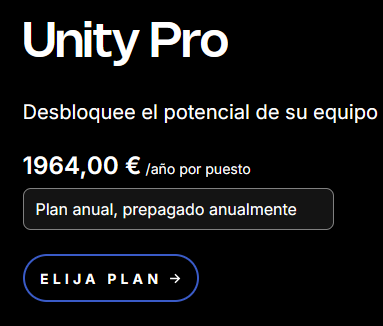
\includegraphics[width=\linewidth]{include/images/unitypro.png}
        \caption{Precio anual de Unity Pro}
        \label{fig:unitypro}
    \end{minipage}
    \hfill
    % ---- SEGUNDA IMAGEN ----
    \begin{minipage}[b]{0.48\linewidth}
        \centering
        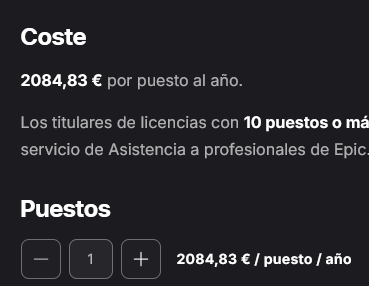
\includegraphics[width=\linewidth]{include/images/unrealenginepro.PNG}
        \caption{Precio anual de Unreal Engine}
        \label{fig:unrealenginepro}
    \end{minipage}
\end{figure}





\item Hardware para testing: Dispositivos móviles de diferentes gamas, gafas AR (HoloLens, Magic Leap) y VR (Quest, Vive) para pruebas exhaustivas. Inversión inicial: 10.000-15.000€.
\item Marketing y ventas: Campañas publicitarias, participación en ferias, material promocional, equipo comercial. Coste variable: 10.000-30.000€/año inicialmente.
\item Legal y administrativo: Registro de empresa, asesoría legal para contratos, cumplimiento GDPR, seguros profesionales. Coste estimado: 5.000-8.000€/año.
\end{itemize}
- \textbf{Métricas claves}: Para evaluar el éxito y evolución del proyecto, se monitorizarán las siguientes métricas:
\begin{itemize}
\item Usuarios activos mensuales: Número de profesionales que utilizan efectivamente la aplicación al menos una vez al mes, diferenciando entre usuarios gratuitos y de pago.
\item Tasa de conversión freemium-premium: Porcentaje de usuarios que migran del plan gratuito a suscripciones de pago, indicador fundamental de la percepción de valor añadido.
\item Tiempo medio de uso por sesión: Métrica que refleja el "compromiso" real con la aplicación; sesiones muy cortas podrían indicar problemas de usabilidad o falta de utilidad percibida.
\item \gls{nps}: Índice de satisfacción que mide la probabilidad de que los usuarios recomienden la aplicación a amigos, crucial en un mercado \gls{b2b} donde la prescripción profesional es determinante.
\item Reducción de errores constructivos detectados: Métrica cualitativa obtenida mediante encuestas a usuarios, que cuantifica el impacto real en la eficiencia de los proyectos.
\item \gls{cac} vs \gls{ltv}: Ratio que determina la sostenibilidad económica del modelo, indicando si el coste de adquisición de cada cliente es inferior al valor que aporta durante su ciclo de vida.
\item Tasa de retención mensual: Porcentaje de usuarios que continúan utilizando la aplicación mes a mes, indicador de la solidez del producto y la fidelización conseguida.
\end{itemize}
- \textbf{Ventaja diferencial}: Los elementos que diferencian esta propuesta de las soluciones competidoras existentes son:
\begin{itemize}
\item A diferencia de herramientas especializadas solo en presentación a clientes o solo en inspección de obra, esta aplicación cubre todas las fases desde el diseño inicial hasta la ejecución final con una única plataforma coherente.
\item Accesibilidad tecnológica: Funciona con gafas convencionales para AR (no requiere equipamiento caro como HoloLens) y ofrece experiencias VR en gafas de gama media, democratizando el acceso frente a soluciones enterprise de alto coste.
\item Experiencia de usuario simplificada: Curva de aprendizaje mínima mediante interfaces intuitivas diseñadas para profesionales no técnicos, eliminando la barrera de entrada que presentan herramientas complejas que requieren formación extensiva.
\end{itemize}

\begin{table}[!htb]
\centering
\caption{Lean Canvas del proyecto}
\label{tab:lean-canvas}
\resizebox{\textwidth}{!}{
\footnotesize
\begin{tabular}{|>{\raggedright\arraybackslash\hspace{0pt}}p{2.8cm}|>{\raggedright\arraybackslash\hspace{0pt}}p{2.8cm}|>{\raggedright\arraybackslash\hspace{0pt}}p{2.8cm}|>{\raggedright\arraybackslash\hspace{0pt}}p{2.8cm}|>{\raggedright\arraybackslash\hspace{0pt}}p{2.8cm}|}
\hline
\textbf{PROBLEMA} & \textbf{SOLUCIÓN} & \textbf{PROPUESTA DE VALOR ÚNICA} & \textbf{VENTAJA DIFERENCIAL} & \textbf{SEGMENTOS DE CLIENTE} \\
\hline
\begin{itemize}[leftmargin=*,noitemsep,topsep=2pt,itemsep=4pt]
    \item Dificultad para comunicar proyectos a clientes no técnicos
    \item Errores constructivos no detectados a tiempo
    \item Falta de herramientas intuitivas para inspección
    \item Barreras en colaboración multidisciplinar
    \item Limitaciones de herramientas actuales
\end{itemize}
&
\begin{itemize}[leftmargin=*,noitemsep,topsep=2pt,itemsep=4pt]
    \item App VR para gafas de realidad virtual
    \item Sistema de importación BIM (IFC, Revit)
    \item Anotación y reporte
    \item Modo colaborativo
\end{itemize}
&
\begin{itemize}[leftmargin=*,noitemsep,topsep=2pt,itemsep=4pt]
    \item Integración AR/VR accesible sin ser experto.
\end{itemize}
&
\begin{itemize}[leftmargin=*,noitemsep,topsep=2pt,itemsep=4pt]
    \item Integración completa AR y/o VR
    \item Interoperabilidad BIM real
    \item Experiencia de usuario simplificada
\end{itemize}
&
\begin{itemize}[leftmargin=*,noitemsep,topsep=2pt,itemsep=4pt]
    \item Estudios de arquitectura e ingeniería
    \item Empresas constructoras
    \item Promotoras inmobiliarias
    \item Project managers
    \item Centros formativos
\end{itemize}
\\
\hline
& \textbf{MÉTRICAS CLAVE} & & \textbf{CANALES} & \\
\cline{2-2} \cline{4-4}
&
\begin{itemize}[leftmargin=*,noitemsep,topsep=2pt,itemsep=3pt]
    \item Usuarios activos mensuales (MAU)
    \item Conversión freemium/premium
    \item Tiempo uso por sesión
    \item Net Promoter Score
    \item Reducción errores detectados
    \item CAC vs LTV
    \item Retención mensual
\end{itemize}
& &
\begin{itemize}[leftmargin=*,noitemsep,topsep=2pt,itemsep=3pt]
    \item Ferias y congresos sector
    \item Colaboración fabricantes BIM
    \item Marketing digital (LinkedIn)
    \item Prescripción universitaria
    \item Casos de éxito
\end{itemize}
& \\
\hline
\multicolumn{3}{|c|}{%
    \begin{minipage}[t]{\dimexpr 8.4cm + 4\tabcolsep + 2\arrayrulewidth\relax}
        \vspace{0.15cm}
        \textbf{ESTRUCTURA DE COSTES} \par \vspace{0.1cm}
        \begin{itemize}[leftmargin=*,noitemsep,topsep=0pt,itemsep=3pt]
            \item Desarrollo software (50.000-80.000€ MVP)
            \item Licencias software (3.000-5.000€/año)
            \item Hardware testing (10.000-15.000€)
            \item Marketing (10.000-30.000€/año)
            \item Legal y administrativo (5.000-8.000€/año)
        \end{itemize}
        \vspace{0.15cm}
    \end{minipage}%
} & 
\multicolumn{2}{c|}{%
    \begin{minipage}[t]{\dimexpr 5.6cm + 2\tabcolsep + \arrayrulewidth\relax}
        \vspace{0.15cm}
        \textbf{FLUJOS DE INGRESOS} \par \vspace{0.1cm}
        \begin{itemize}[leftmargin=*,noitemsep,topsep=0pt,itemsep=3pt]
            \item Suscripción freemium: básico gratuito, profesional 15-30€/mes, empresarial personalizado
            \item Licencias educativas
            \item Servicios profesionales (consultoría, formación)
            \item Marketplace de contenidos
        \end{itemize}
        \vspace{0.15cm}
    \end{minipage}%
} \\
\hline
\end{tabular}
}
\end{table}


\section{Análisis de riesgos} 

El análisis de riesgos, visto en el Cuadro~\ref{tab:riesgos} permite identificar anticipadamente aquellos eventos o circunstancias que podrían impactar negativamente en el desarrollo del proyecto, evaluando su probabilidad de ocurrencia y su potencial impacto\footnote{\cite{pmi2017pmbok}}. A diferencia del análisis DAFO que examina amenazas externas de forma general, este apartado se centra en riesgos concretos con estrategias específicas de mitigación. Esta herramienta permitirá aumentar significativamente las probabilidades de éxito del proyecto, anticipando problemas antes de que se materialicen y estableciendo planes de contingencia para aquellos que, inevitablemente, surgirán durante el desarrollo.

- \textbf{Riesgos técnicos}:
\begin{itemize}
\item Rendimiento insuficiente en dispositivos móviles: Los modelos BIM de proyectos arquitectónicos reales pueden contener miles de polígonos, lo que podría saturar la capacidad de procesamiento de smartphones de gama media.
    Probabilidad: Media-Alta
    Impacto: Alto (experiencia de usuario degradada)
    Mitigación: Implementar sistemas de optimización automática (Level of Detail, occlusion culling), establecer límites técnicos claros para la complejidad de modelos soportados y desarrollar algoritmos de simplificación geométrica que preserven la fidelidad visual.
\item Incompatibilidades entre formatos BIM y Point Cloud: A pesar de la existencia del estándar IFC, las exportaciones desde diferentes software presentan inconsistencias que podrían generar errores al importar modelos.
    Probabilidad: Media
    Impacto: Medio (requiere corrección manual)
    Mitigación: Desarrollar validadores robustos que detecten inconsistencias, proporcionar herramientas de corrección semiautomática y mantener documentación clara sobre mejores prácticas de exportación desde los principales software BIM.
\end{itemize}
- \textbf{Riesgos de planificación}:
\begin{itemize}
\item Subestimación de la complejidad técnica: La curva de aprendizaje en desarrollo AR/VR podría consumir más tiempo del previsto, retrasando hitos importantes del proyecto.
    Probabilidad: Alta
    Impacto: Medio (retraso en entregas)
    Mitigación: Establecer un calendario realista con margen de contingencia, priorizar funcionalidades core mediante metodología \gls{moscow} y validar la viabilidad técnica de aspectos críticos mediante prototipos tempranos.

\item Dispersión de objetivos: La amplitud de funcionalidades posibles podría llevar a intentar abarcar demasiado, resultando en un producto superficial que no destaque en ningún aspecto.
    Probabilidad: Media
    Impacto: Alto (producto poco competitivo)
    Mitigación: Definir claramente la base con 3-4 funcionalidades core bien implementadas antes de considerar expansiones, validar cada adición mediante criterios objetivos de valor añadido y resistir la tentación de implementar "características interesantes" que no resuelvan problemas reales.
\end{itemize}

- \textbf{Riesgos de mercado}:
\begin{itemize}
\item Rechazo por parte del público objetivo: Los profesionales del sector podrían percibir la solución como un "gadget tecnológico" sin valor práctico real, especialmente si la curva de aprendizaje supera los beneficios percibidos.
    Probabilidad: Media
    Impacto: Crítico (producto sin adopción)
    Mitigación: Involucrar usuarios potenciales desde fases tempranas mediante entrevistas y sesiones de testing, diseñar la interfaz con feedback, y mostrar casos de uso con métricas concretas de ahorro de tiempo o reducción de errores.

\item Movimientos competitivos: Grandes empresas del sector BIM (Autodesk, Trimble) podrían lanzar funcionalidades similares integradas en sus plataformas establecidas, haciendo redundante esta solución independiente.

    Probabilidad: Media
    Impacto: Alto (competencia con recursos superiores)
    Mitigación: Enfocarse en tópicos desatendidos con soluciones para pequeños estudios, mantener ventajas en interoperabilidad y experiencia de usuario simplificada, y considerar estrategias de colaboración o integración en lugar de competencia directa.
\end{itemize}
Riesgos operativos:
\begin{itemize}
\item Dependencia de plataformas externas: Cambios en políticas de Apple (ARKit) o Google (ARCore), modificaciones o incrementos de costes de servicios podrían afectar significativamente al proyecto.
    Probabilidad: Baja-Media
    Impacto: Medio-Alto (requiere adaptaciones urgentes)
    Mitigación: Diseñar arquitectura modular que permita sustituir componentes externos, mantenerse informado sobre los planes de plataformas tecnológicas clave y considerar opciones open-source.

\item Problemas de seguridad y privacidad: Una vulnerabilidad que exponga datos sensibles de proyectos constructivos podría generar responsabilidades legales y dañar irreparablemente la reputación.
    Probabilidad: Baja (con buenas prácticas)
    Impacto: Crítico (consecuencias legales y reputacionales)
    Mitigación: Implementar cifrado end-to-end para datos sensibles, realizar auditorías de seguridad regulares, cumplir estrictamente con GDPR y normativas de protección de datos, y contratar seguros de responsabilidad profesional si el proyecto evoluciona más allá del ámbito académico.
\end{itemize}

\begin{table}[!htb]
\centering
\caption{Matriz de riesgos del proyecto}
\label{tab:riesgos}
\resizebox{\textwidth}{!}{
\begin{tabular}{>{\raggedright\arraybackslash\hspace{0pt}}p{4.5cm}ccc>{\raggedright\arraybackslash\hspace{0pt}}p{5.5cm}}
\toprule
\textbf{Riesgo} & \textbf{Probabilidad} & \textbf{Impacto} & \textbf{Prioridad} & \textbf{Estrategia} \\
\midrule
Rendimiento insuficiente en móviles & Media-Alta & Alto & Alta & Optimización técnica proactiva \\
\addlinespace
Subestimación complejidad & Alta & Medio & Alta & Planificación conservadora + MVP \\
\addlinespace
Rechazo usuarios objetivo & Media & Crítico & Alta & Validación temprana con usuarios \\
\addlinespace
Incompatibilidades BIM & Media & Medio & Media & Validadores robustos \\
\addlinespace
Movimientos competitivos & Media & Alto & Media & Diferenciación por nicho \\
\addlinespace
Dispersión de objetivos & Media & Alto & Media & Priorización estricta MVP \\
\addlinespace
Dependencia plataformas & Baja-Media & Medio-Alto & Media & Arquitectura modular \\
\addlinespace
Vulnerabilidades seguridad & Baja & Crítico & Alta & Buenas prácticas + auditorías \\
\bottomrule
\end{tabular}
}
\end{table}	% Plantilla: Se muestran listas
\chapter{\label{planificacion}Planificación}


En este apartado se establece la distribución de tiempo prevista para cada fase del trabajo, con el objetivo de presentarlo en la convocatoria de septiembre de 2026. Cada etapa incluye una estimación de duración y una fecha límite orientativa que servirá como referencia para evaluar el progreso y detectar posibles desviaciones.

Las estimaciones tienen en cuenta los riesgos identificados previamente en la matriz de riesgos, particularmente aquellos relacionados con la curva de aprendizaje en tecnologías AR/VR y la posible subestimación de la complejidad técnica. Además, se ha considerado la carga académica que supone el ABP, lo que reduce la disponibilidad efectiva de horas semanales dedicables al proyecto.

Se ha incorporado un margen de seguridad de dos semanas antes de la fecha límite oficial de entrega, previendo la aparición de imprevistos técnicos, problemas con hardware de testing o cualquier otra contingencia que pudiera surgir durante el desarrollo.

El inicio oficial del proyecto tuvo lugar el 22 de diciembre de 2025, fecha con la que se empezó a investigar herramientas técnicas y se comenzó la redacción de la memoria. Todos estos plazos se detalla en el siguiente Cuadro~\ref{tab:planificacion-temporal}. 


\begin{table}[!htb]
\centering
\caption{Planificación temporal del proyecto}
\label{tab:planificacion-temporal}
\begin{tabular}{p{8cm}cc}
\toprule
\textbf{Contenidos} & \textbf{Tiempo estimado} & \textbf{Fecha límite} \\
\midrule
Motivación, Introducción, Estudio de viabilidad & 2 semanas & 12/01/2026 \\
\addlinespace
Planificación, Estado del arte, Objetivos, Metodología & 3 semanas & 26/01/2026 \\
\addlinespace
Análisis y especificación & 3 semanas & 16/02/2026 \\
\addlinespace
Diseño & 4 semanas & 09/03/2026 \\
\addlinespace
Implementación & 10 semanas & 06/04/2026 \\
\addlinespace
Pruebas y validación, Resultados & 4 semanas & 15/06/2026 \\
\addlinespace
Conclusiones y trabajo futuro, Referencias, bibliografía y apéndices, Revisión final & 3 semanas & 06/07/2026 \\
\bottomrule
\end{tabular}
\end{table}




\chapter{\label{estado-arte}Estado del arte}

La intersección entre tecnologías inmersivas (Realidad Aumentada y Realidad Virtual) y el sector de la construcción representa un campo en constante evolución que ha experimentado un crecimiento significativo durante la última década. Para abordar adecuadamente el desarrollo de una aplicación AR/VR orientada a la visualización de proyectos arquitectónicos mediante modelos BIM, resulta imprescindible comprender el contexto tecnológico actual, las soluciones existentes en el mercado, sus fortalezas y limitaciones, así como las tendencias emergentes que están configurando el futuro del sector.

Esta sección consiste en un análisis exhaustivo del estado actual de la técnica, examinando tanto los fundamentos tecnológicos que sustentan estas aplicaciones como las propuestas comerciales y académicas más relevantes. El objetivo es adquirir una visión comprehensiva que permita identificar oportunidades de mejora, detectar funcionalidades desatendidas y establecer los requisitos técnicos necesarios para diseñar una solución que aporte valor real diferenciado.

\section{Reconstrucción volumétrica: 3D Gaussian Splatting}

El 3D Gaussian Splatting (3DGS) ha emergido recientemente como una técnica revolucionaria para la reconstrucción tridimensional y el renderizado volumétrico a partir de un conjunto de fotografías bidimensionales. A diferencia de la modelado tradicional, que intenta generar mallas poligonales cerradas y a menudo falla al interpretar superficies reflectantes, transparentes o sin textura, el 3DGS representa la escena utilizando millones de partículas matemáticas (distribuciones gaussianas 3D) que poseen atributos de posición, escala, rotación, opacidad y color armónico esférico.

Esta técnica es considerado un salto considerable respecto a métodos previos como los NeRFs (Neural Radiance Fields). Mientras que los NeRFs requieren tiempos de inferencia altísimos que imposibilitan su uso fluido\footnote{\cite{mildenhall2020nerf}}, el Gaussian Splatting permite un renderizado fotorrealista en tiempo real, alcanzando mejores tasas de fotogramas (FPS) incluso en escenas de gran complejidad geométrica.

En el contexto de la arquitectura y la construcción, esta tecnología ofrece posibilidades para el control de calidad y la auditoría de obras:

Como se puede observar en la Figura~\ref{fig:gaussian-splat}, Gaussian Splatting permite digitalizar el estado actual de una obra o apartamento con un fotorrealismo absoluto, capturando detalles milimétricos (como cableado, texturas de materiales o imperfecciones) que los escáneres láser o las mallas tradicionales suelen ignorar o deformar.

Adicionalmente, la verdadera potencia de esta tecnología en el sector constructivo reside en su superposición con los modelos teóricos. Al importar una captura de Gaussian Splatting en un entorno inmersivo junto al modelo BIM original, los profesionales pueden realizar una inspección visual directa, detectando desviaciones, errores de ejecución o interferencias estructurales antes de que supongan un sobrecoste crítico para el proyecto.


La integración de nubes de puntos volumétricas generadas mediante 3DGS como entorno de validación para modelos BIM resuelve de manera directa los conflictos existentes entre el diseño digital planificado y la realidad física construida.

\begin{figure}[!htb]
    \centering
    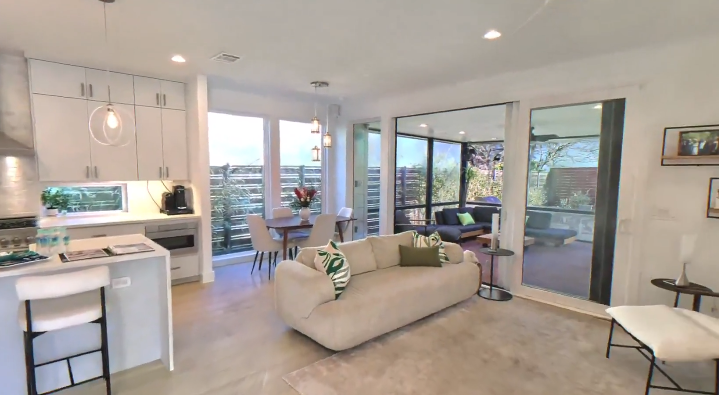
\includegraphics[width=0.8\linewidth]{include/images/figura3.1.PNG}
    \caption{Comparación Gaussian Splat con realidad}
    \label{fig:gaussian-splat}
\end{figure}


\begin{figure}[!htb]
    \centering
    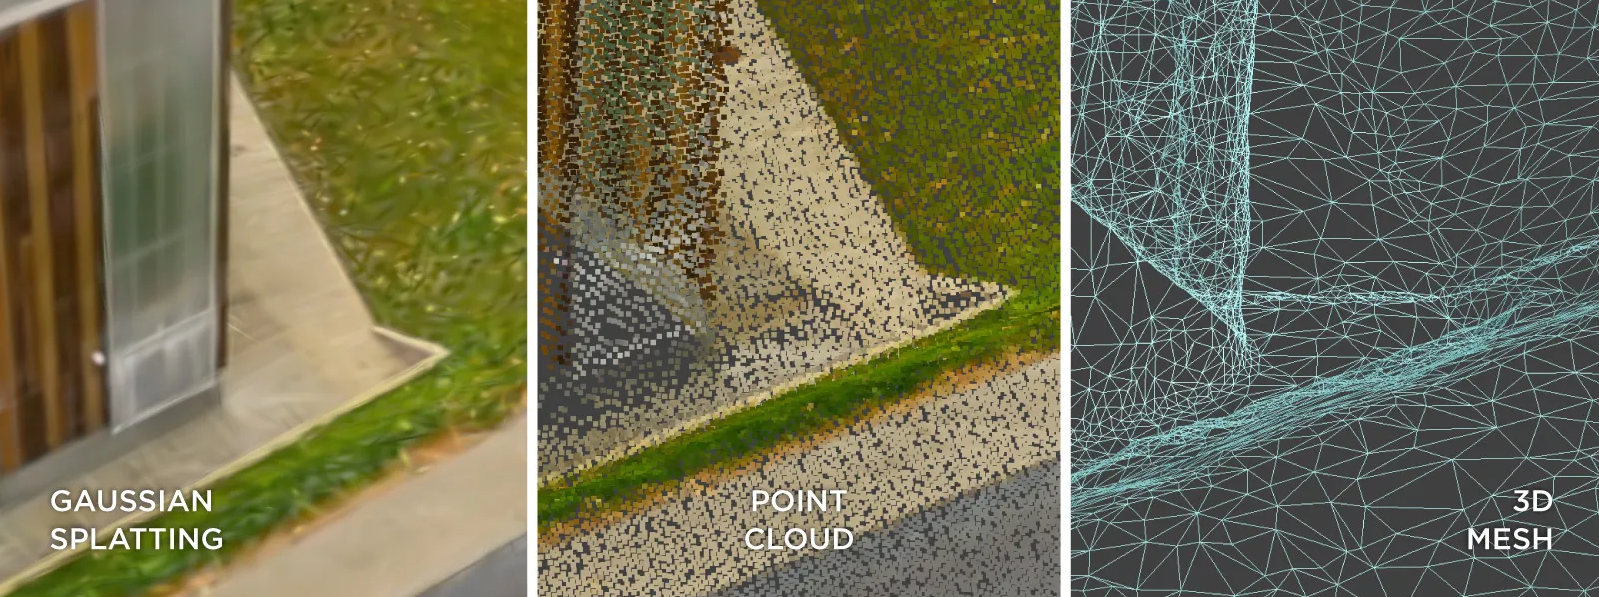
\includegraphics[width=0.8\linewidth]{include/images/gaussiancomparison.png}
    \caption{Comparación de Gaussian Splat, Point Cloud convencional y malla 3D}
    \label{fig:gaussiancomparison}
\end{figure}

\section{Metodología BIM en la construcción}
Building Information Modeling (BIM) representa un cambio paradigmático en la forma de concebir, diseñar y ejecutar proyectos de construcción\footnote{\cite{eastman2011bim}}. A diferencia de los métodos tradicionales basados en planos bidimensionales independientes, BIM propone un modelo tridimensional único y centralizado que integra información geométrica, técnica, funcional y temporal de todos los elementos constructivos.
\begin{figure}[!htb]
    \centering
    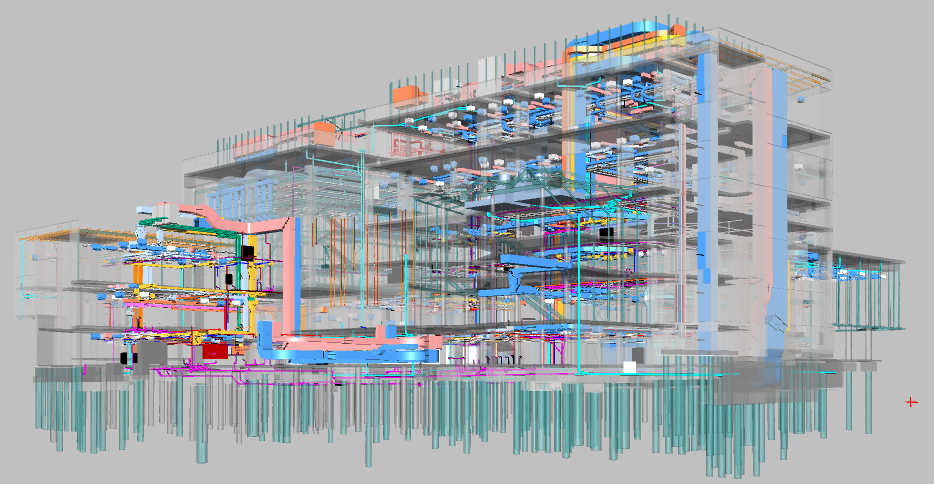
\includegraphics[width=0.8\linewidth]{include/images/BIMmodel.png}
    \caption{Edificio BIM clasificado en elementos constructivos}
    \label{fig:BIMmodel}
\end{figure}
\subsection{Evolución y adopción BIM}

La adopción de metodologías BIM ha sido progresiva pero constante. Países como Reino Unido establecieron en 2016 la obligatoriedad de utilizar BIM nivel 2 en proyectos públicos\footnote{\cite{ukcabinet2016strategy}}, mientras que la Unión Europea publicó en 2017 el manual para la introducción del BIM en contratación pública\footnote{\cite{eubim2017handbook}}. En España, aunque la implantación ha sido más gradual, la Comisión BIM creada por el Ministerio de Fomento en 2015 ha impulsado su adopción mediante recomendaciones y directrices, estableciendo diciembre de 2018 como fecha recomendada para su uso en licitaciones públicas\footnote{\cite{fomento2015comision}}.

Esta estandarización progresiva genera un ecosistema propicio para aplicaciones que consuman datos BIM, dado que cada vez más proyectos disponen de modelos digitales estructurados susceptibles de ser visualizados mediante tecnologías inmersivas.

\subsection{Formatos y estándares BIM}

La interoperabilidad constituye uno de los desafíos fundamentales del ecosistema BIM. Diferentes actores del proyecto utilizan software especializado para sus disciplinas (Revit para arquitectura, Tekla para estructuras, MEP para instalaciones), lo que genera la necesidad de formatos de intercambio que preserven la información.

IFC (Industry Foundation Classes) se ha consolidado como el estándar abierto por excelencia, desarrollado por buildingSMART International. IFC define una estructura de datos jerárquica que describe elementos constructivos (muros, forjados, ventanas), sus propiedades (materiales, dimensiones, características térmicas) y relaciones espaciales. Su carácter abierto y neutral respecto a fabricantes lo convierte en la opción preferente para garantizar interoperabilidad, aunque las implementaciones de exportación/importación en diferentes software presentan ocasionalmente inconsistencias.

Otros formatos relevantes incluyen BCF (BIM Collaboration Format) para comunicación de incidencias asociadas a elementos del modelo, COBie (Construction Operations Building Information Exchange) orientado a datos para la gestión de instalaciones, formatos propietarios como .RVT de Autodesk Revit que, aunque no abiertos, están ampliamente extendidos en la industria.

Para aplicaciones AR/VR, la conversión desde estos formatos hacia representaciones optimizadas para renderizado en tiempo real (meshes con texturas, estructuras LOD) constituye un requisito técnico que debe equilibrar fidelidad visual y rendimiento.

\subsection{Niveles de desarrollo LOD}

El concepto de Level of Development (LOD) estandariza el grado de definición geométrica y la cantidad de información asociada a los elementos BIM en diferentes fases del proyecto. La especificación más utilizada, desarrollada y estandarizada globalmente, define distintos niveles de detalle geométrico y semántico\footnote{\cite{eastman2011bim}}:
\begin{itemize}
\item LOD 100: Representación simbólica y conceptual (volúmenes aproximados)
\item LOD 200: Geometría aproximada con dimensiones, orientación y ubicación
\item LOD 300: Geometría precisa con información completa para construcción
\item LOD 400: Geometría detallada para fabricación e instalación
\item LOD 500: Modelo as-built verificado en campo
\end{itemize}

\begin{figure}[!htb]
    \centering
    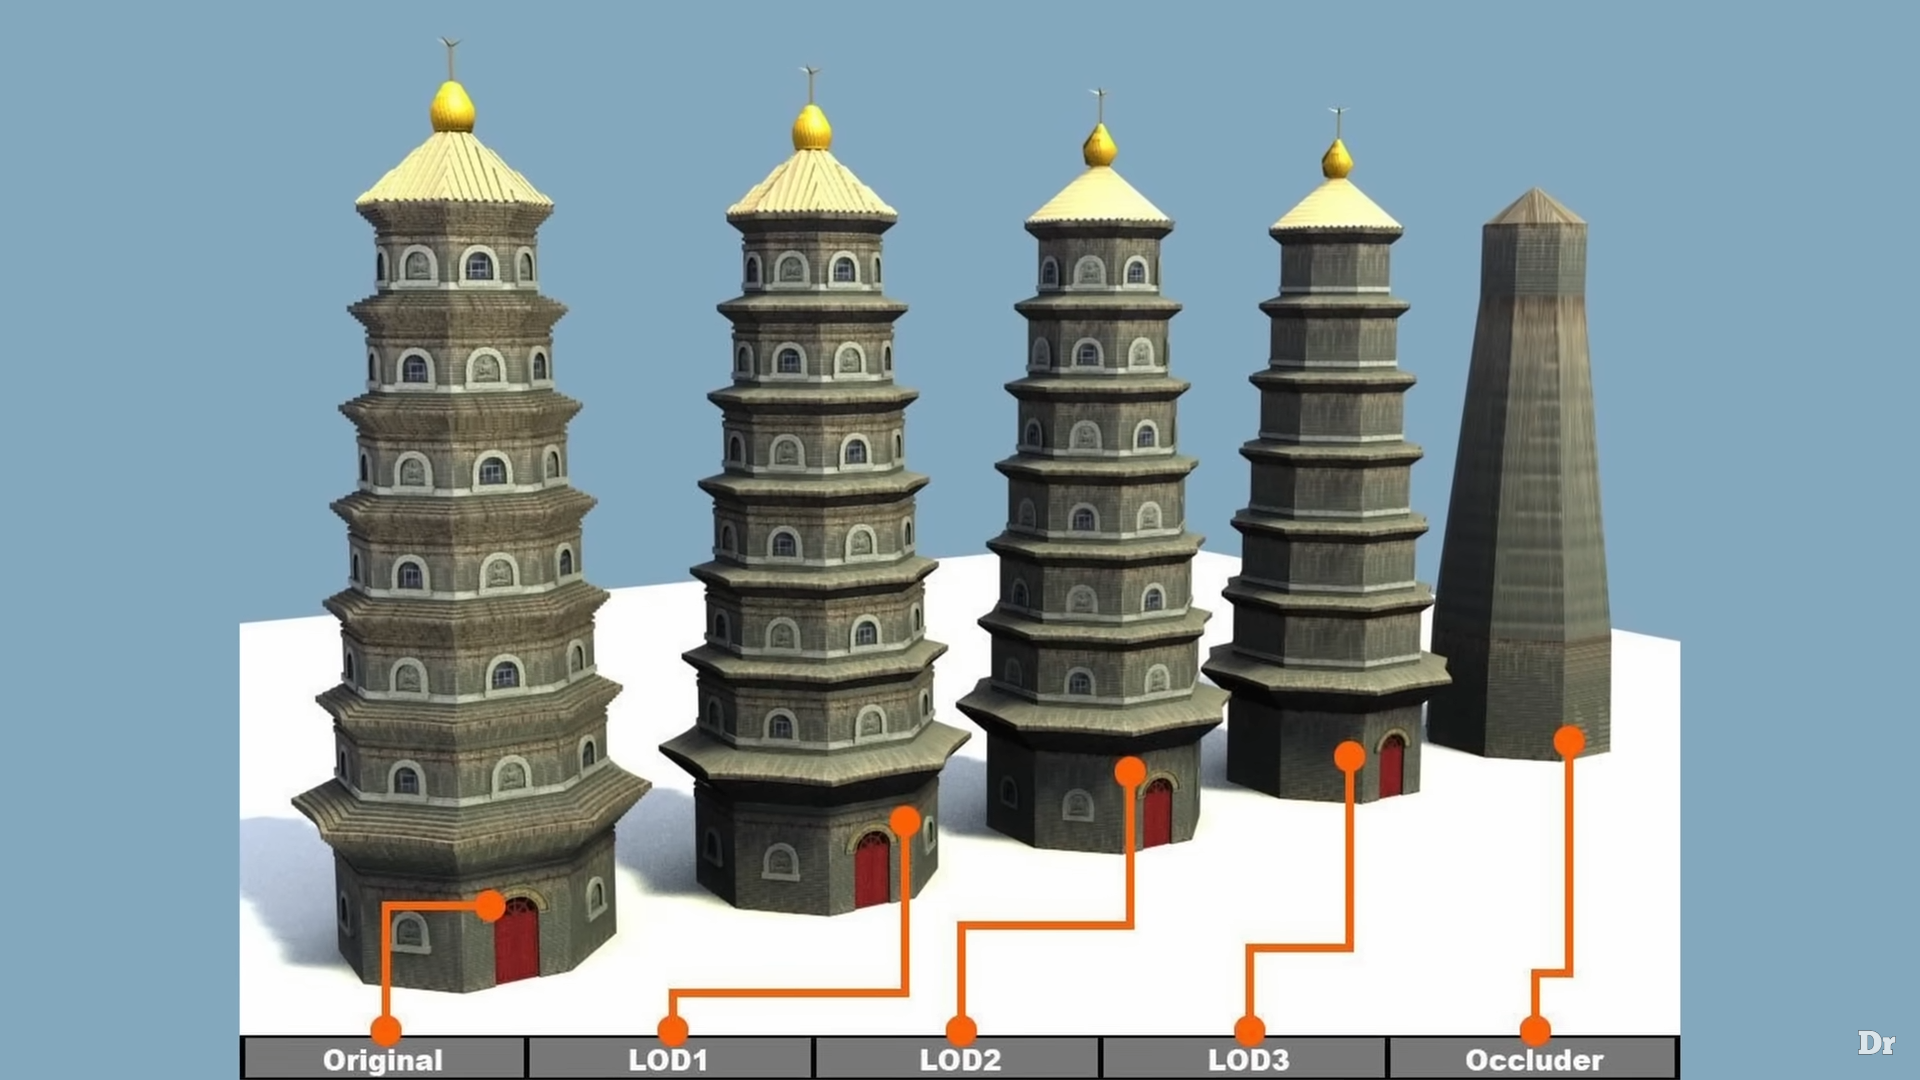
\includegraphics[width=0.8\linewidth]{include/images/lods.png}
    \caption{Ejemplos de tipos de LODs}
    \label{fig:lods}
\end{figure}
Esta gradación resulta relevante para aplicaciones AR/VR porque diferentes casos de uso requieren distintos niveles de detalle. Una presentación comercial a clientes puede funcionar perfectamente con LOD 200-300, mientras que una inspección técnica en obra podría necesitar LOD 400 para verificar encuentros constructivos complejos. Implementar sistemas de visualización que adapten automáticamente el nivel de detalle según el contexto de uso constituye un factor diferenciador importante. Como se puede ver en la siguiente Figura~\ref{fig:BIM-model}, un modelado 3D habitual coge los detalles exteriores del edificio, sin embargo, un modelo BIM analiza cada una de sus partes interiores.

\begin{figure}[!htb]
    \centering
    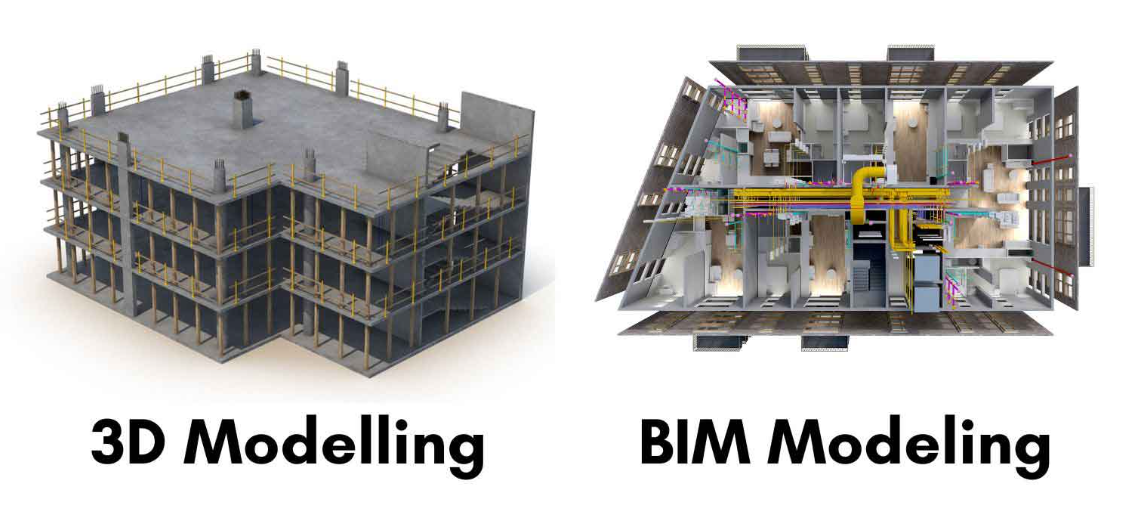
\includegraphics[width=0.8\linewidth]{include/images/figura3.2.png}
    \caption{Diferencia modelado normal con modelado BIM}
    \label{fig:BIM-model}
\end{figure}



\section{Tecnologías de Realidad Aumentada} 
En esta sección se explica toda la parte teórica relacionada con Realidad Aumentada. 
\subsection{Fundamentos técnicos de AR}


La Realidad Aumentada superpone información digital sobre la percepción del mundo real, requiriendo resolver tres desafíos técnicos fundamentales: tracking (determinar posición y orientación del dispositivo en el espacio), mapping (construir representación del entorno) y rendering (generar contenido virtual coherente con la escena real)\footnote{\cite{azuma1997survey}}.

Los sistemas modernos de AR utilizan principalmente dos enfoques de tracking:
\begin{itemize}
\item Marker-based AR: Emplea patrones visuales predefinidos (códigos QR, imágenes) que la cámara reconoce y utiliza como referencia espacial. Ofrece alta precisión en entornos controlados pero requiere preparar y mantener los marcadores físicos, lo que resulta poco práctico en obras de construcción.

\begin{figure}[!htb]
    \centering
    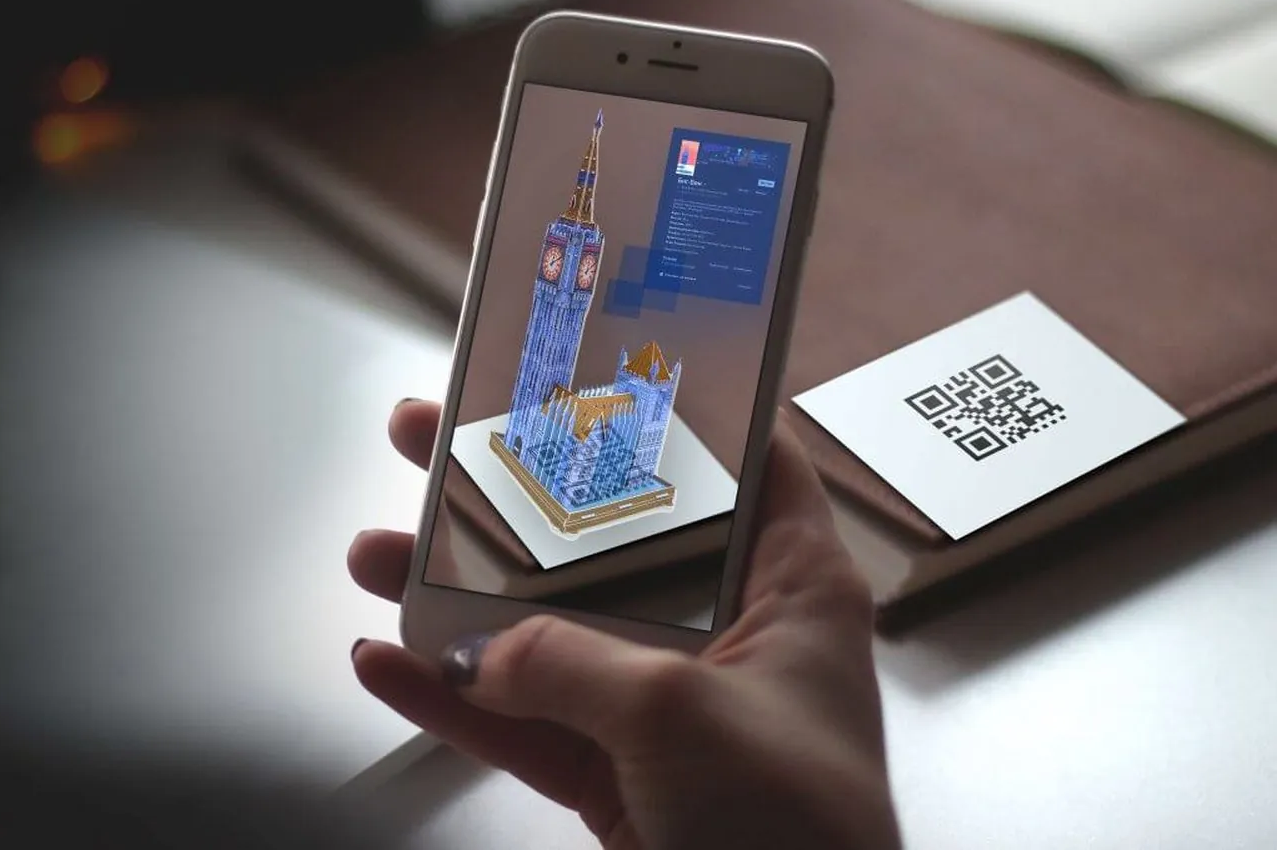
\includegraphics[width=0.8\linewidth]{include/images/markerbased.png}
    \caption{Código QR utilizado como referencia}
    \label{fig:markerbased}
\end{figure}


\item Markerless AR o SLAM: Analiza características naturales del entorno para construir un mapa espacial y posicionar el dispositivo dentro de él, lo cual conlleva desafíos de iluminación y falta de referencias en entornos de construcción\footnote{\cite{rankohi2013review}}. Este enfoque, implementado en ARCore (Google) y ARKit (Apple), permite experiencias más fluidas sin preparación previa, aunque presenta limitaciones de precisión (típicamente 5-10 cm en interiores, mayor error en exteriores).

\begin{figure}[!htb]
    \centering
    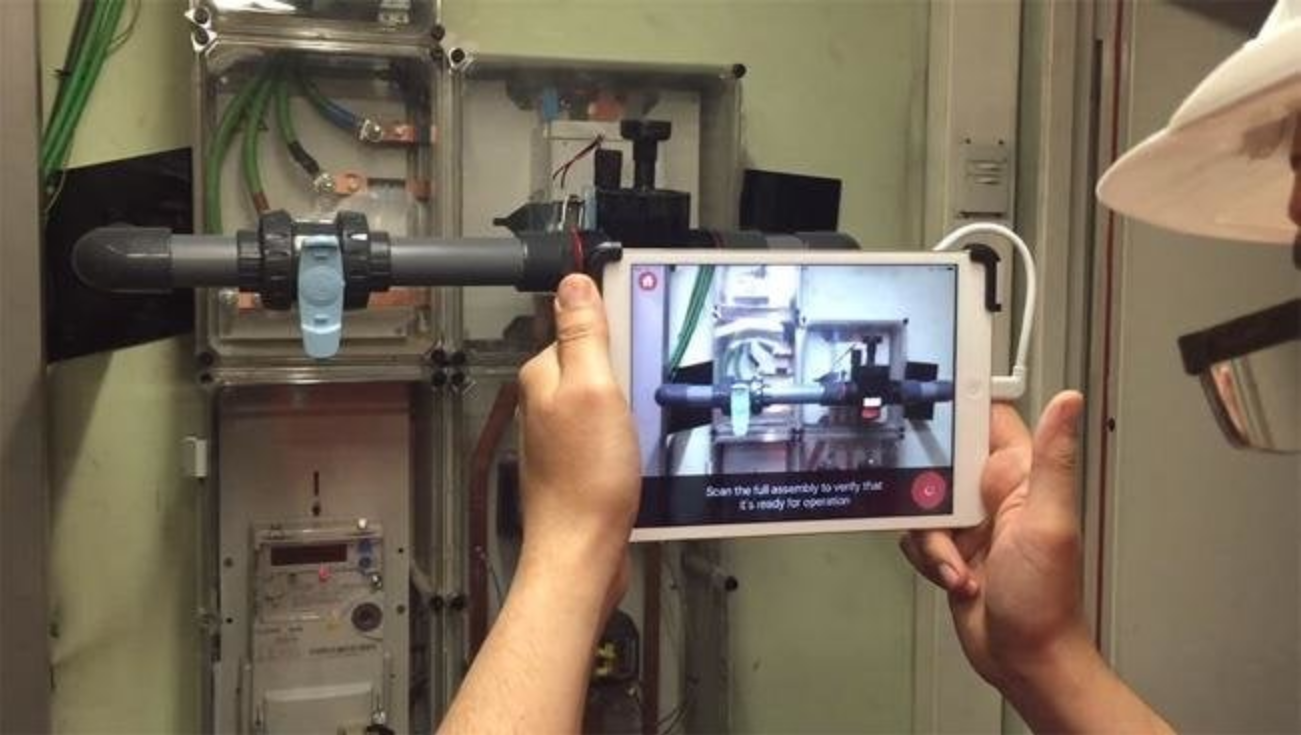
\includegraphics[width=0.8\linewidth]{include/images/markerlessar.png}
    \caption{Realidad aumentada markerless}
    \label{fig:markerlessar}
\end{figure}
\end{itemize}
Para aplicaciones en construcción, frecuentemente se necesita AR en exteriores sobre emplazamientos vacíos sin referencias visuales distintivas.

\subsection{Plataformas de desarrollo AR}

ARCore (Android) y ARKit (iOS) constituyen las plataformas dominantes para AR móvil. Ambas ofrecen APIs para detección de planos horizontales y verticales, estimación de iluminación ambiental, tracking de imágenes y rostros, y anclaje de contenido virtual. Sus capacidades son similares, aunque ARKit tradicionalmente ha mantenido ventaja en precisión de tracking gracias al control más estricto de Apple sobre el hardware.

Para aplicaciones multiplataforma, frameworks como Unity con AR Foundation o Unreal Engine con AR plugins proporcionan una capa de abstracción que permite tener la misma base desplegable en ambos ecosistemas, reduciendo significativamente el esfuerzo de desarrollo y mantenimiento.

Dispositivos especializados como Microsoft Hololens 2 o Magic Leap 2 ofrecen experiencias AR más avanzadas mediantes gafas con displays transparentes, liberando las manos del usuario y proporcionando campos de visión más amplios. Sin embargo, su elevado coste (3000-4000€ por unidad) y menor disponibilidad limitan su adopción masiva, relegándolos a casos de uso profesionales de alto valor añadido.

\begin{figure}[!htb]
    \centering
    % ---- PRIMERA IMAGEN ----
    \begin{minipage}[b]{0.48\linewidth}
        \centering
        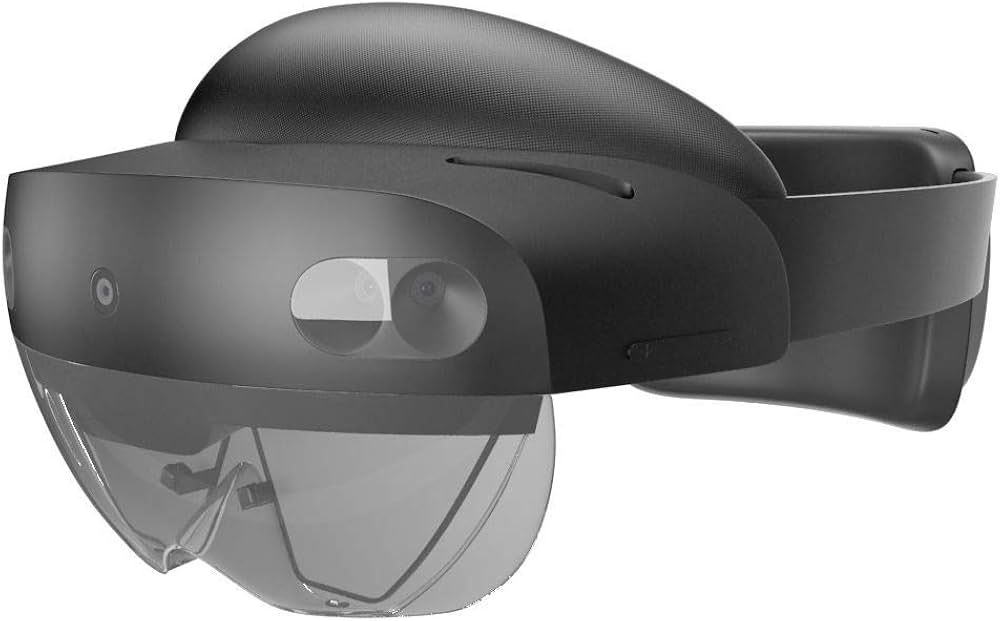
\includegraphics[width=\linewidth]{include/images/microsoftlens2.jpg}
        \caption{Gafas microsoft Lens 2}
        \label{fig:microsoftlens2}
    \end{minipage}
    \hfill
    % ---- SEGUNDA IMAGEN ----
    \begin{minipage}[b]{0.48\linewidth}
        \centering
        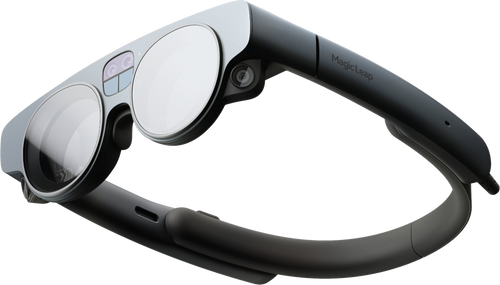
\includegraphics[width=\linewidth]{include/images/magicleap2.png}
        \caption{Gafas Magid Leap 2}
        \label{fig:magicleap2}
    \end{minipage}
\end{figure}

\subsection{Desafíos específicos de AR en construcción}

La aplicación de AR en entornos de construcción presenta particularidades que no aparecen en otros dominios:
\begin{itemize}

\item Condiciones ambientales adversas: Obras expuestas a polvo, variaciones lumínicas extremas (sol directo, sombra), lluvia o temperaturas extremas que afectan al rendimiento de cámaras y sensores.

\item Ausencia de referencias visuales: En fases tempranas, el emplazamiento puede ser un solar vacío sin características distintivas, obligando a depender de GPS con sus limitaciones de precisión\footnote{\cite{wang2013augmented}}.

\item Escala y distancias: Los proyectos arquitectónicos abarcan decenas o cientos de metros, mientras que el tracking AR optimiza para espacios interiores de pocos metros. Mantener coherencia espacial en áreas extensas requiere estrategias específicas de gestión de anclajes persistentes.

\item Complejidad geométrica: Los modelos BIM contienen millones de polígonos que superan las capacidades de renderizado en tiempo real de dispositivos móviles, necesitando técnicas agresivas de optimización (culling, LOD dinámico, instancing).
\end{itemize}
Solucionar estos desafíos constituye uno de los valores añadidos fundamentales que debe aportar una aplicación AR específicamente diseñada para construcción.


\section{Tecnologías de Realidad Virtual}
En esta sección se explica toda la parte teórica relacionada con Realidad Virtual.
\subsection{Fundamentos técnicos de VR}



La Realidad Virtual sumerge completamente al usuario en un entorno sintético mediante headsets que bloquean la visión del mundo real y presentan imágenes estereoscópicas (ligeramente diferentes para cada ojo) que generan percepción de profundidad tridimensional.

Los sistemas VR modernos ofrecen 6 grados de libertad (6DoF), tracking tanto de la orientación de la cabeza (pitch, yaw, roll) como de su posición espacial (x, y, z) permitiendo al usuario moverse naturalmente por el entorno virtual\footnote{\cite{slater2009place}}. Esto contrasta con sistemas más simples de 3DoF que solo rastrean orientación, adecuados para experiencias pasivas (visualización 360º) pero limitados para exploración activa de espacios arquitectónicos.

Los principales desafíos técnicos de VR incluyen:
\begin{itemize}
\item Latencia motora-visual: El retardo entre movimiento de cabeza y actualización de la imagen debe mantenerse por debajo de 20ms para evitar mareo. Esto exige mantener framerates elevados incluso con escenas complejas.

\item Resolución y field of view: Los displays actuales (típicamente 1832x1920 por ojo en Meta Quest 2) muestra efecto de pixelado ("screen door effect") que rompe la inmersión. Aumentar resolución compite con las demandas de framerate.

\item Ergonomía y comfort: Sesiones prolongadas pueden causar fatiga ocular, mareo (motion sickness) o incomodidad por el peso del dispositivo. El diseño de interacciones debe minimizar estos efectos mediante técnicas como teleportación en lugar de movimiento continuo con joystick en casos extremos de optimización.
\end{itemize}
\subsection{Plataformas VR y dispositivos}

El mercado VR se ha consolidado en torno a varios ecosistemas principales:
\begin{itemize}
\item Meta Quest (anteriormente Oculus) lidera en dispositivos standalone (todo incluido sin necesidad de PC), ofreciendo experiencias inalámbricas a precios asequibles (300-500€). Su capacidad de procesamiento limitada exige optimización agresiva de contenidos.

\begin{figure}[!htb]
    \centering
    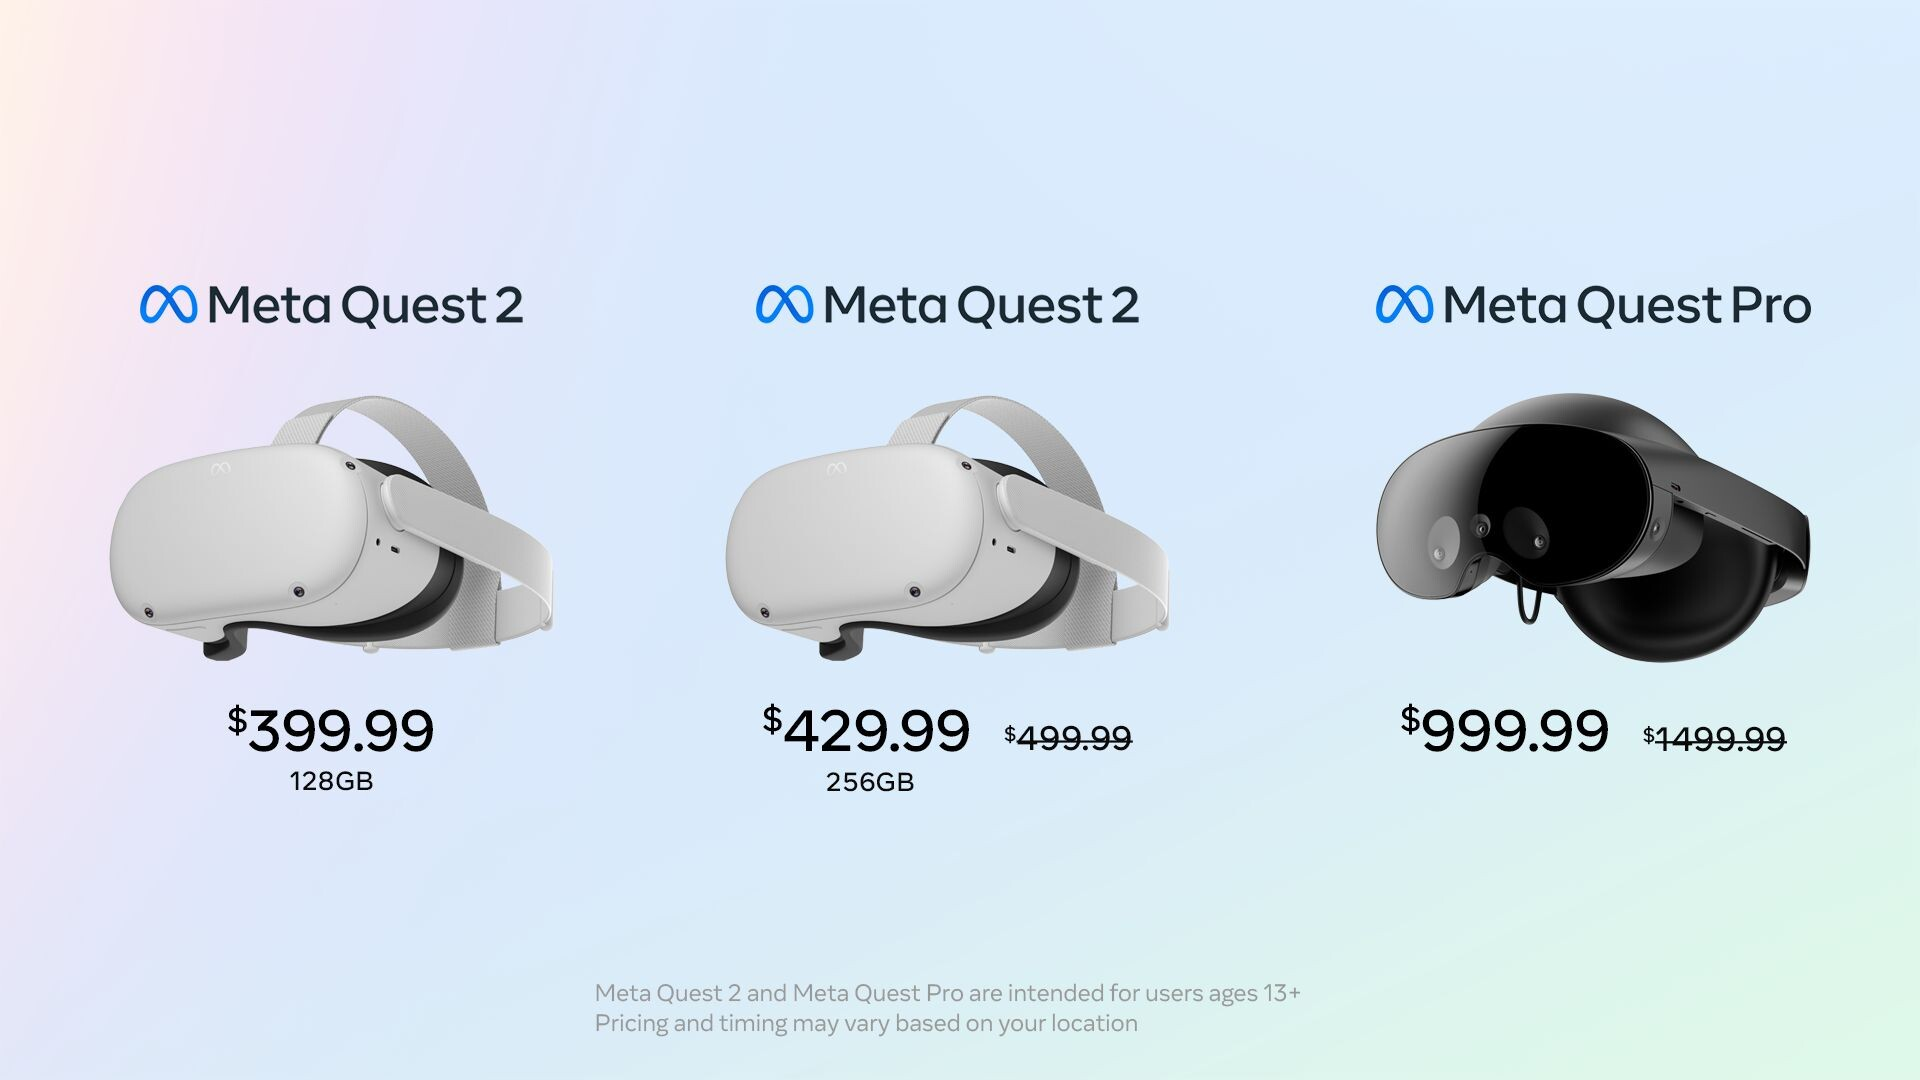
\includegraphics[width=0.8\linewidth]{include/images/questheadsets.jpg}
    \caption{Gafas de realidad virtual y precio de Meta Quest (2 y Pro)}
    \label{fig:questheadsets}
\end{figure}

\item HTC Vive/Valve Index: Representan la gama alta de VR conectada a PC, ofreciendo mayor fidelidad visual, tracking más preciso mediante estaciones base externas y controllers más avanzados, al coste de instalación más compleja y presupuestos superiores (800-1500€).

\begin{figure}[!htb]
    \centering
    % ---- PRIMERA IMAGEN ----
    \begin{minipage}[b]{0.48\linewidth}
        \centering
        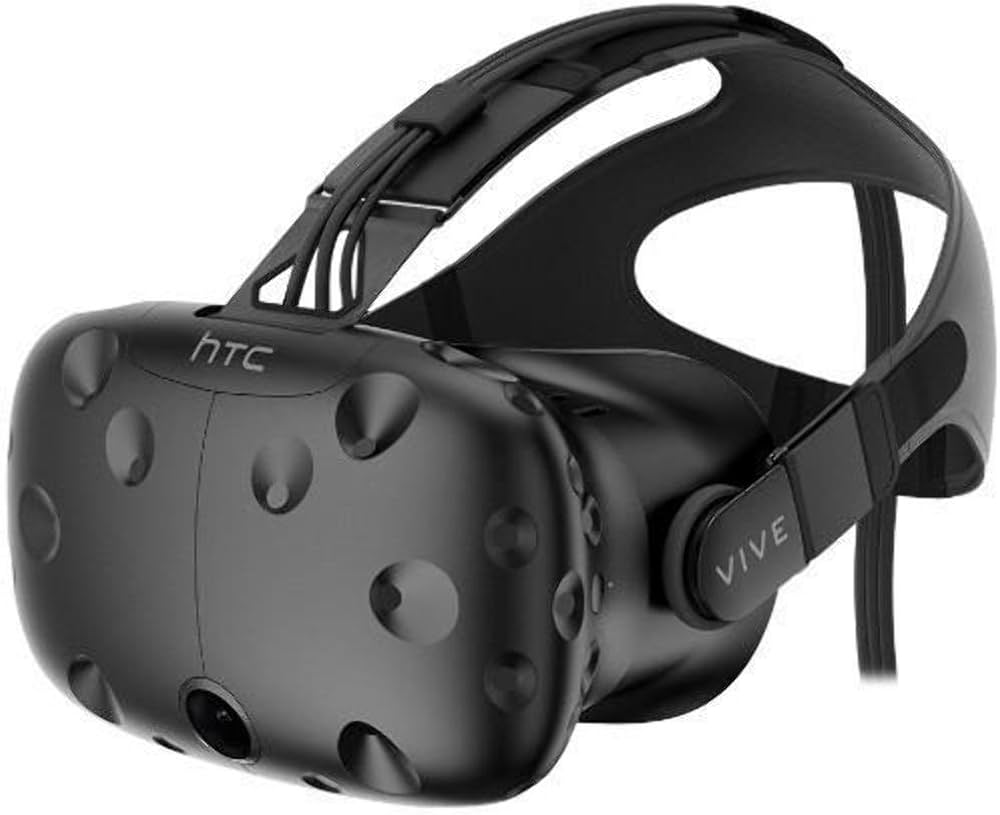
\includegraphics[width=\linewidth]{include/images/htcvive.jpg}
        \caption{Gafas HTC Vive}
        \label{fig:htcvive}
    \end{minipage}
    \hfill
    % ---- SEGUNDA IMAGEN ----
    \begin{minipage}[b]{0.48\linewidth}
        \centering
        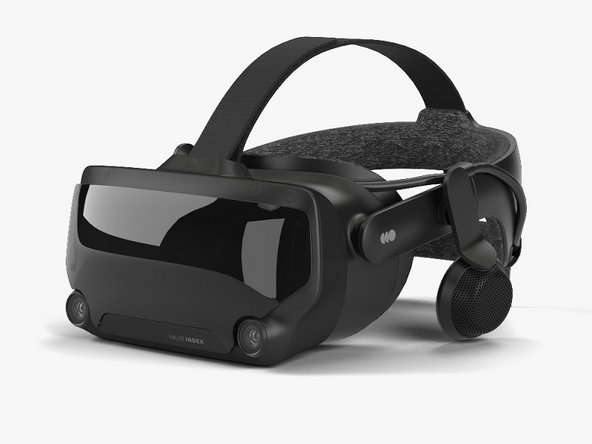
\includegraphics[width=\linewidth]{include/images/valveindex.jpg}
        \caption{Gafas Valve Index}
        \label{fig:valveindex}
    \end{minipage}
\end{figure}

\item PlayStation VR: Captura el mercado de consolas pero resulta menos relevante para aplicaciones profesionales por sus capacidades limitadas y ecosistema cerrado.

\begin{figure}[!htb]
    \centering
    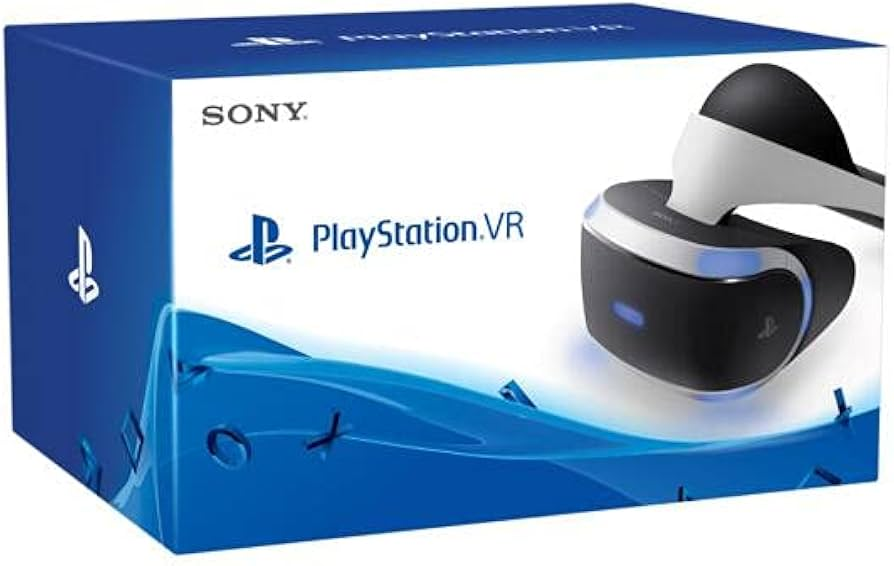
\includegraphics[width=0.8\linewidth]{include/images/psvr.jpg}
    \caption{Gafas Playstation VR}
    \label{fig:psvr}
\end{figure}


\item Pico (propiedad de ByteDance): Emerge como alternativa a Meta en mercados empresariales, ofreciendo dispositivos standalone con enfoque business y gestión de flotas.

\begin{figure}[!htb]
    \centering
    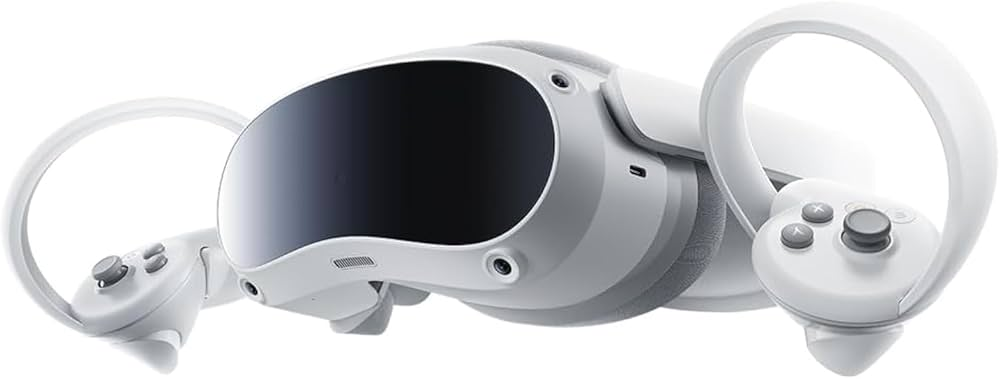
\includegraphics[width=0.8\linewidth]{include/images/pico4.jpg}
    \caption{Gafas Pico 4}
    \label{fig:pico}
\end{figure}


\end{itemize}
Para desarrollo multiplataforma, Unity y Unreal Engine vuelven a ser las opciones dominantes, soportando todos los headsets principales mediante OpenXR, el estándar abierto para VR impulsado por Khronos Group que permite desarrollar una vez y desplegar en múltiples dispositivos.

\subsection{VR aplicada a arquitectura y construcción}

VR resulta particularmente valiosa en construcción para:

- Visualización de proyectos: Permitir a clientes, inversores o autoridades experimentar espacios antes de su construcción, evaluando proporciones, iluminación natural, vistas y sensación espacial de forma imposible mediante renders estáticos o vídeos.

- Revisión de diseño: Arquitectos e ingenieros pueden detectar conflictos espaciales, evaluar ergonomía de circulaciones y validar parámetros de seguridad desde la perspectiva del usuario final\footnote{\cite{li2018critical}}.

- Formación en seguridad: Simulación de procedimientos de trabajo en altura, manejo de maquinaria o respuesta ante emergencias en entornos controlados sin riesgos reales.

- Coordinación de oficios: Visualización de instalaciones (electricidad, fontanería, climatización) en su contexto espacial real facilita detectar interferencias antes de ejecutar en obra.

Las ventajas de VR complementan las de AR: mientras AR destaca en validación in-situ sobre lo construido, VR sobresale en exploración de lo aún no construido y en contextos donde el desplazamiento físico resultaría costoso o impracticable.

\section{Análisis de soluciones existentes}
En esta sección se detallarán las aplicaciones actuales más similares a los que se pretende abarcar este proyecto.
\subsection{Fuzor: VR + BIM}

Fuzor, desarrollado por Kalloc Studios, constituye una de las propuestas más consolidadas de integración BIM-VR. Su enfoque principal es servir como visualizador inmersivo de modelos Revit (como se puede observar en la Figura~\ref{fig:Fuzor-screenshot}), estableciendo un vínculo directo (LiveLink) que sincroniza cambios en el modelo BIM con la representación VR en tiempo real\footnote{\cite{fuzor}}.

Características principales:
\begin{itemize} 
\item Integración nativa con Autodesk Revit mediante plugin
\item Soporte de múltiples headsets VR (HTC Vive, OCulus, WIndows MR)
\item Funcionalidades de clash detection (detección de colisiones) visualizadas en VR.
\item Simulación de secuencias constructivas.
\item Herramientas de medición y anotación dentro del entorno virtual.
\item Motor físico para simulación de comportamiento de objetos.
\end{itemize}
La sincronización en tiempo real con Revit representa su mayor ventaja competitiva, permitiendo a diseñadores iterar sobre el proyecto y evaluar cambios inmediatamente en VR sin exportaciones intermedias. Las capacidades de simulación 4D resultan valiosas para planificación de obra.

Sin embargo, su dependencia de Revit limita la interoperabilidad con flujos de trabajo basados en otros software BIM. No ofrece funcionalidades AR robustas para uso en campo, centrándose casi exclusivamente en VR de escritorio. El precio (licencia anual de aproximadamente 500-800€ por usuario) puede resultar prohibitivo para estudios pequeños. La curva de aprendizaje es pronunciada, requiriendo formación específica para aprovechar todas las funcionalidades.

\begin{figure}[!htb]
    \centering
    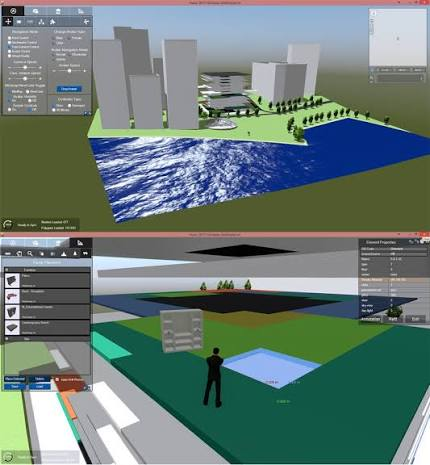
\includegraphics[width=0.7\linewidth]{include/images/figura3.3.jpg}
    \caption{Captura realizada en Fuzor}
    \label{fig:Fuzor-screenshot}
\end{figure}

\subsection{Trimble Connect: AR en construcción}

Trimble Connect forma parte del ecosistema de soluciones constructivas de Trimble, multinacional especializada en tecnologías de posicionamiento y gestión de proyectos. Como se puede apreciar en la Figura~\ref{fig:Trimble-screenshot} Su aplicación móvil AR permite visualizar modelos BIM directamente sobre el emplazamiento real mediante smartphones o tablets\footnote{\cite{trimbleconnect}}.

Caracteristicas principales:
\begin{itemize}
\item Aplicación móvil para iOS y Android
\item Importación de modelos desde múltiples fuentes BIM (Revit, SketchUp, Tekla)
\item Posicionamiento mediante GPS y alineación manual
\item Herramientas de medición y comparación modelo vs realidad
\item Sistema de issues/incidencias geolocalizadas
\item Integración con plataforma Trimble Connect para colaboración en nube
\end{itemize}
Su integración con el ecosistema Trimble (estaciones totales, escáneres láser, soluciones de topografía) proporciona ventajas significativas para empresas que ya utilizan estos equipamientos profesionales. La aplicación móvil resulta más accesible que soluciones basadas en gafas AR caras. El sistema de gestión de incidencias vinculado al modelo facilita la comunicación entre oficina técnica y obra.

Por otro lado, la precisión de posicionamiento mediante GPS resulta insuficiente para muchas tareas de inspección detallada. La interfaz, aunque funcional, no destaca por su intuitividad y requiere cierto periodo de adaptación. Las funcionalidades más avanzadas requiere suscripción a servicios Trimble Connect, generando costes recurrentes. No ofrece experiencias VR inmersivas, limitándose a AR móvil.

\begin{figure}[!htb]
    \centering
    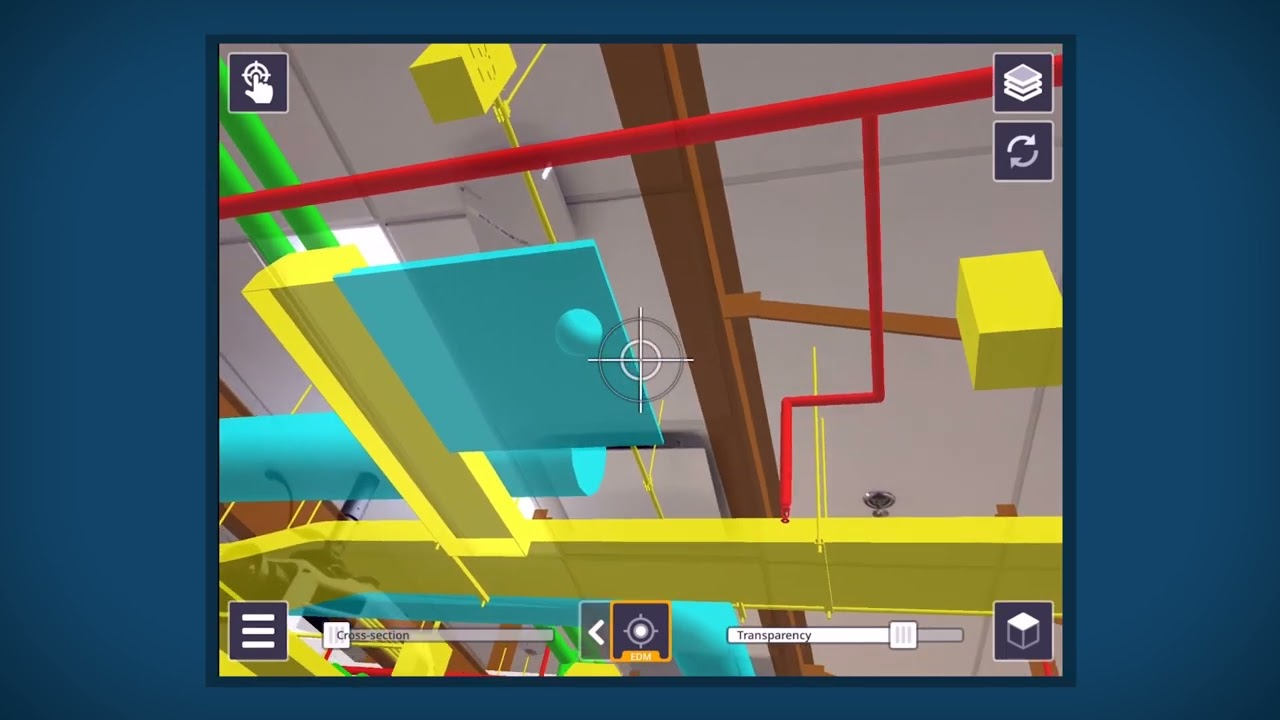
\includegraphics[width=0.7\linewidth]{include/images/figura3.4.jpg}
    \caption{Captura realizada en la aplicación móvil de Trimble}
    \label{fig:Trimble-screenshot}
\end{figure}

\subsection{IrisVR Prospect: inmersión VR multiusuario}

IrisVR Prospect (posteriormente adquirida por Techstars y actualmente parte de Resolve BIM) se especializó en crear experiencias VR de alta calidad a partir de modelos BIM, con particular énfasis en sesiones colaborativas multiusuario.

Características principales:
\begin{itemize}
\item Conversión automática de modelos BIM (Revit, Navisworks, Rhino, SketchUp) a entornos VR
\item Soporte de headsets principales (Oculus, Vive, Windows MR)
\item Modo multiusuario para reuniones virtuales dentro del modelo
\item Herramientas de medición, anotación y captura de vistas
\item Simulación de variantes de diseño (materiales, colores, configuraciones)
\item Exportación de recorridos VR para presentaciones
\end{itemize}
La calidad visual de las escenas generadas destaca sobre competidores, notándose sobre todo en materiales realistas e iluminación. Las sesiones multiusuario permiten reuniones de coordinación donde múltiples participantes (arquitectos, clientes, contratistas) exploran conjuntamente el modelo, cada uno desde su ubicación física, señalando elementos y discutiendo en tiempo real mediante audio espacializado. La simplicidad del flujo de trabajo, que consiste en importar un modelo, para después tenerlo automáticamente disponible en VR reduce barreras de entrada.

En cambio, no incluye funcionalidades AR, siendo exclusivamente una solución VR. Requiere hardware potente (PC gaming o estaciones de trabajo) para modelos complejos, limitando la portabilidad. La suscripción resulta costosa (aproximadamente 70/100€ mes por usuario), especialmente para uso ocasional. Tras la adquisición por Resolve, el desarrollo independiente de Prospect cesó, integrándose sus capacidades en la plataforma más amplia de Resolve BIM.
\subsection{Resolve BIM: plataforma integrada de coordinación}

Resolve (anteriormente conocida como BIM Track hasta 2020) representa una evolución hacia plataformas integrales que unifican coordinación BIM, gestión de incidencias y visualización inmersiva\footnote{\cite{resolvebim}}. Tras adquirir IrisVR en 2021, Resolve integró las capacidades VR de Prospect en su ecosistema más amplio de gestión de proyectos constructivos.

Características principales:
\begin{itemize} 

\item Plataforma cloud centralizada para coordinación BIM multiproyecto
\item Sistema avanzado de gestión de issues con workflows personalizables
\item Visualización 3D web (sin necesidad de software específico) de modelos BIM
\item Módulo VR heredado de IrisVR Prospect para inmersión y reuniones virtuales, mostrado en la Figura~\ref{fig:ResolveBIM-screenshot}
\item Clash detection (detección de colisiones) con priorización inteligente
\item Integración con Revit, Navisworks, Solibri y otros software BIM mediante plugins
\item Sistema de reportes y analíticas sobre estado del proyecto
\item Aplicación móvil para consulta y resolución de incidencias en campo
\end{itemize}
La principal ventaja de Resolve radica en su enfoque holístico, no es simplemente una herramienta de visualización AR/VR, sino una plataforma completa de gestión que incluye capacidades inmersivas como un componente más del flujo de trabajo. Esto facilita la trazabilidad completa desde la detección de un conflicto en VR hasta su asignación, seguimiento y verificación de resolución. El sistema de issues es particularmente robusto, con clasificación por disciplinas, estados, responsables y prioridades, generando dashboards ejecutivos que proporcionan visibilidad del estado global del proyecto.

La visualización web 3D representa otra fortaleza significativa, cualquier stakeholder con navegador puede explorar el modelo sin instalar software especializado ni tener conocimientos técnicos avanzados. Esto democratiza el acceso a la información del proyecto, facilitando la colaboración con clientes, autoridades regulatorias o subcontratistas que no manejan software BIM.

El módulo VR, aunque derivado de IrisVR Prospect, se integra perfectamente con el resto de la plataforma, las incidencias detectadas durante sesiones VR se crean automáticamente en el sistema de gestión, asignan a responsables y rastrean hasta su cierre, cerrando el ciclo de coordinación.

A pesar de sus virtudes, Resolve presenta limitaciones importantes para ciertos casos de uso. No ofrece funcionalidades AR móvil para inspección en obra, centrándose en coordinación de oficina técnica. La experiencia VR, aunque integrada, no ha evolucionado significativamente desde la adquisición de IrisVR, manteniendo las mismas limitaciones de requerir PC potente y headset dedicado.

El modelo de negocio basado en suscripción por proyecto (no solo por usuario) puede resultar costoso para estudios que manejan múltiples proyectos simultáneamente pequeños. La complejidad de la plataforma, si bien justificada por su amplitud funcional, genera curvas de aprendizaje pronunciadas que requieren inversión en formación para aprovechamiento óptimo.

Otra limitación destacable es la dependencia de conectividad, trabajar sin conexión a internet resulta problemático, lo cual puede ser restrictivo en obras donde la conectividad es inestable o inexistente. Aunque existe aplicación móvil, sus capacidades están limitadas principalmente a consulta y anotación básica, sin permitir acceder a todas las funcionalidades disponibles en la versión desktop.

Finalmente, la integración VR heredada de IrisVR no aprovecha las tendencias más recientes como headsets standalone (requiere conexión a PC), realidad mixta o funcionalidades colaborativas AR, manteniéndose como una solución VR "tradicional" en un mercado que evoluciona rápidamente hacia experiencias más versátiles.

\begin{figure}[!htb]
    \centering
    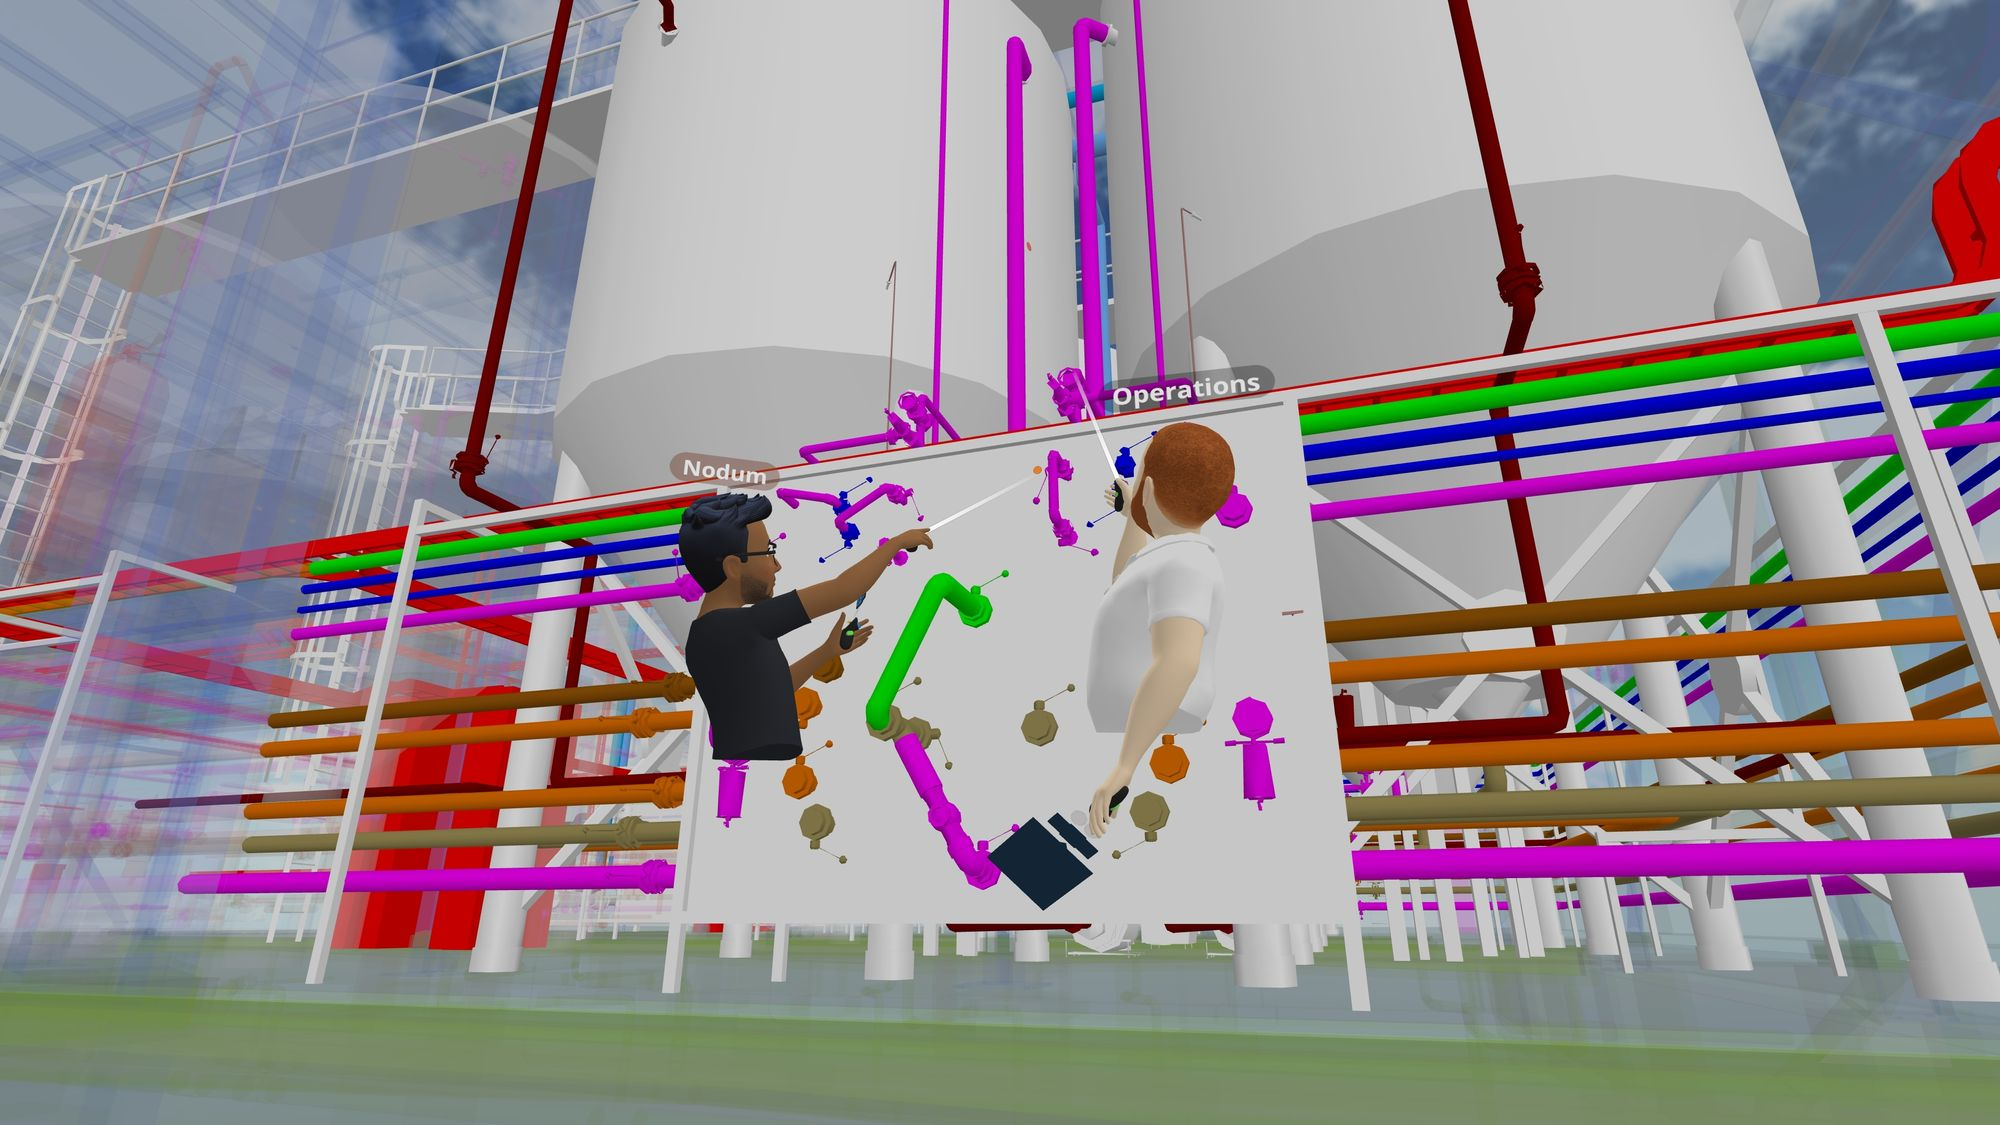
\includegraphics[width=0.8\linewidth]{include/images/figura3.5.jpg}
    \caption{Captura realizada en ResolveBIM}
    \label{fig:ResolveBIM-screenshot}
\end{figure}




\subsection{Análisis comparativo}

\begin{table}[!htb]
\centering
\caption{Análisis comparativo de soluciones existentes}
\label{tab:comparativa-soluciones}
\small
\begin{tabular}{p{4cm}cccc}
\toprule
\textbf{Característica} & \textbf{Fuzor} & \textbf{Trimble} & \textbf{IrisVR} & \textbf{Resolve} \\
\midrule
Soporte AR móvil & No & Sí & No & No \\
\addlinespace
Soporte VR & Sí (excelente) & No & Sí (excelente) & Sí (bueno) \\
\addlinespace
Integración Revit & Directa & Importación & Importación & Plugin \\
\addlinespace
Interoperabilidad BIM & Limitada & Amplia & Amplia & Amplia \\
\addlinespace
Colaboración multiusuario & Limitada & Sí (cloud) & Sí (VR) & Sí (cloud + VR) \\
\addlinespace
Gestión de issues & Básica & Buena & Básica & Excelente \\
\addlinespace
Uso en campo/obra & No & Sí (móvil) & No & Limitado \\
\addlinespace
Visualización web & No & Sí (básica) & No & Sí (avanzada) \\
\addlinespace
Curva aprendizaje & Pronunciada & Media & Suave & Pronunciada \\
\addlinespace
Coste & Alto & Medio & Alto & Alto \\
\addlinespace
Precisión posicionamiento & N/A & Media (GPS) & N/A & N/A \\
\addlinespace
Enfoque principal & VR & AR campo & VR & Gestión integral \\
\bottomrule
\end{tabular}
\end{table}


Ninguna de las soluciones analizadas en el Cuadro~\ref{tab:comparativa-soluciones} cubre completamente el espectro de necesidades identificado. Fuzor e IrisVR destacan en VR pero no ofrecen AR móvil para uso en obra. Trimble Connect proporciona AR en campo pero carece de experiencias VR inmersivas. Resolve BIM ofrece la plataforma de gestión más completa e integra VR, pero no incluye capacidades AR para inspección en campo y presenta barreras de entrada significativas en coste y complejidad.

Todas las soluciones presentan limitaciones en accesibilidad (coste, curva de aprendizaje o requisitos hardware) que restringen su adopción por pequeños estudios o profesionales independientes, configurando un espacio de oportunidad para propuestas más equilibradas que integren AR y VR manteniendo usabilidad y costes controlados.

\section{Tendencias emergentes y oportunidades}
En esta sección se explicará algunas técnicas de desarrollo para optimizar el uso de las técnologías inmersivas.
\subsection{Realidad mixta (MR) y pass-through AR}

Dispositivos recientes como Meta Quest Pro o Apple Vision Pro difuminan la frontera entre AR y VR mediante pass-through de alta calidad: cámaras frontales capturan el entorno real y lo presentan en los displays del headset, sobre el cual se superpone contenido virtual\footnote{\cite{milgram1994taxonomy}}. Esto permite transiciones fluidas entre inmersión total (VR) y el entorno real (AR) sin cambiar de dispositivo.

Esta convergencia tecnológica abre oportunidades para aplicaciones híbridas que combinen exploración VR de modelos BIM con validación AR sobre lo construido, todo dentro de un mismo flujo de trabajo y dispositivo.
\subsection{Inteligencia artificial aplicada a BIM}

El procesamiento de modelos BIM mediante técnicas de machine learning permite automatizar tareas tediosas como:\footnote{\cite{pan2021artificial}} 
\begin{itemize}
    
\item Simplificación inteligente de geometrías preservando características relevantes
\item Detección automática de conflictos más allá de colisiones geométricas (normativa, constructibilidad)
\item Generación de rutas óptimas de recorrido virtual según criterios personalizables
\item Clasificación automática de elementos para aplicar LODs diferenciados
\end{itemize}
Integrar estas capacidades en una aplicación AR/VR mejoraría significativamente la experiencia de usuario reduciendo intervención manual.

\subsection{Gemelos digitales (Digital Twins)}

El concepto de gemelos digitales extiende BIM más allá de la fase de diseño y construcción, consisten en mantener un modelo digital actualizado durante toda la vida útil del edificio, con todos sus detalles. Sensores IoT (temperatura, humedad, ocupación, consumo energético) alimentan el modelo con datos en tiempo real, dotando de semántica al espacio tridimensional\footnote{\cite{boje2020towards}}. En la Figura~\ref{fig:Gemelos-digitales} se puede apreciar y entender mejor el concepto, consiste en una réplica exacta no física.

Visualizar estos digital twins mediante AR/VR permitiría a gestores de instalaciones ver información operativa contextualizada espacialmente: "esta sala está a 26°C según el sensor, superando el umbral configurado". Esta convergencia BIM-IoT-AR representa una tendencia de crecimiento significativo en la gestión de las instalaciones.


\begin{figure}[!htb]
    \centering
    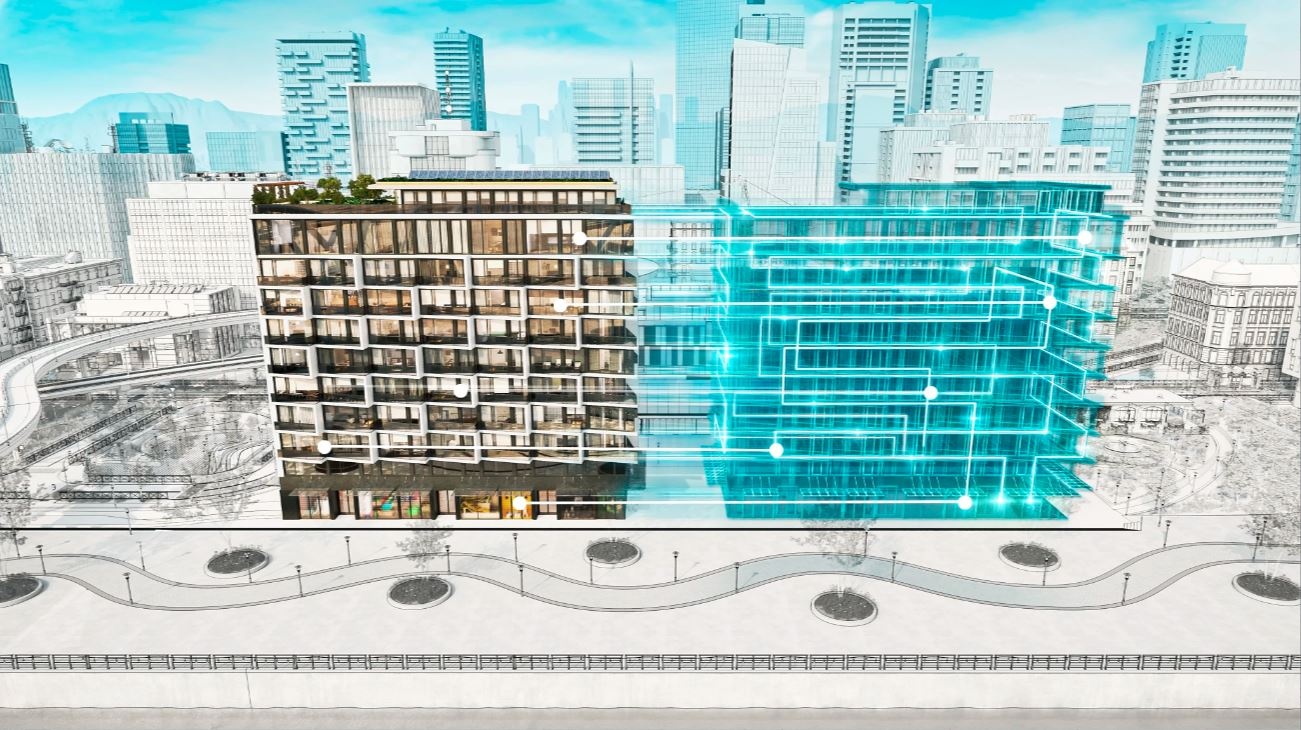
\includegraphics[width=0.8\linewidth]{include/images/figura3.6.jpg}
    \caption{Gemelos digitales}
    \label{fig:Gemelos-digitales}
\end{figure}

\subsection{5G y edge computing}

La latencia reducida y ancho de banda aumentado de redes 5G habilita arquitecturas de renderizado en la nube donde el procesamiento gráfico pesado se ejecuta en servidores y solo se transmite el vídeo resultante al dispositivo móvil. Esto permitiría visualizar modelos BIM complejos en smartphones de gama media, democratizando el acceso a experiencias de alta calidad sin depender de hardware costoso.

Combinado con edge computing (procesamiento cerca del usuario), se podrían ofrecer experiencias colaborativas multiusuario en tiempo real sin las limitaciones actuales de sincronización.

\section{Conclusiones del estado del arte}

El análisis realizado revela un panorama tecnológico maduro en sus fundamentos (AR, VR, BIM) pero que todavía está fragmentado en su aplicación práctica al sector construcción. Las soluciones comerciales existentes destacan en aspectos específicos pero ninguna integra de forma óptima AR móvil para campo, VR inmersiva para diseño y presentación, e interoperabilidad BIM amplia, manteniendo simultáneamente accesibilidad (coste, usabilidad) para pequeños y medianos profesionales.

Esta situación configura un espacio de oportunidad claro para una propuesta que:
\begin{itemize}

\item Priorice interoperabilidad mediante soporte robusto de IFC y otros formatos abiertos.
\item Ofrezca tanto experiencias AR (móvil, accesible) como VR (inmersiva, impactante) con flujo de trabajo unificado.
\item Implemente técnicas avanzadas de optimización para manejar modelos BIM complejos en hardware modesto.
\item Diseñe interfaces específicamente para usuarios del sector (arquitectos, ingenieros, constructores) minimizando curva de aprendizaje.
\item Adopte modelo de negocio accesible (freemium con funcionalidades core gratuitas) que reduzca barreras de entrada.
\end{itemize}

Los fundamentos tecnológicos están disponibles y maduros. Las metodologías BIM están consolidándose como estándar industrial. Los dispositivos AR/VR son cada vez más accesibles y potentes. El conocimiento adquirido sobre el estado del arte proporciona la base necesaria para diseñar una solución que aprenda de los aciertos y evite las limitaciones de propuestas anteriores, aportando valor diferencial real al sector de la construcción.


















\chapter{\label{objetivos}Objetivos}

En este apartado se establecen las metas y finalidades que guiarán el desarrollo del proyecto, definiendo su alcance y propósito. Se presenta primero el objetivo general, seguido de una serie de objetivos específicos que delimitan las diferentes áreas de trabajo necesarias para alcanzar el resultado esperado.

El objetivo principal de este Trabajo de Fin de Grado es diseñar, desarrollar e implementar una aplicación multiplataforma que integre tecnologías de Realidad Aumentada y Realidad Virtual para la visualización, validación e inspección de proyectos arquitectónicos mediante modelos BIM, facilitando la comunicación entre profesionales del sector construcción, mejorando la detección temprana de errores y democratizando el acceso a tecnologías inmersivas en el ámbito de la edificación. Los objetivos específicos son los siguientes:

\begin{itemize}
\item Investigar y dominar los fundamentos técnicos de las tecnologías AR/VR, adquiriendo competencias en frameworks de desarrollo (Unity con AR Foundation), sistemas de tracking espacial y optimización de renderizado en tiempo real para dispositivos móviles/gafas de Realidad Virtual.
\item Comprender en profundidad la metodología BIM y los estándares de intercambio de información en el sector construcción, familiarizándose con el formato IFC, niveles de desarrollo LOD y flujos de trabajo típicos en estudios de arquitectura e ingeniería.
\item Desarrollar un sistema robusto de importación y optimización de modelos BIM que permita convertir archivos IFC en representaciones 3D optimizadas para visualización AR/VR en dispositivos con capacidades de procesamiento limitadas.
\item Implementar funcionalidades AR móviles que permitan superponer modelos BIM sobre emplazamientos reales, utilizando posicionamiento GPS combinado con alineación manual para garantizar precisión suficiente en contextos de obra.
\item Implementar experiencias VR inmersivas que faciliten la exploración virtual de proyectos arquitectónicos antes de su construcción, proporcionando herramientas de navegación intuitivas y sistemas de interacción naturales.
\item Incorporar herramientas de anotación y reporte que permitan a los usuarios marcar discrepancias, añadir comentarios y capturar evidencias fotográficas directamente sobre los modelos visualizados, generando documentación estructurada útil para coordinación de equipos.
\item Diseñar interfaces de usuario intuitivas y específicas para profesionales del sector construcción, minimizando la curva de aprendizaje y priorizando la usabilidad en condiciones reales de trabajo (campo, obra, reuniones con clientes).
\item Garantizar la interoperabilidad mediante estándares abiertos, evitando dependencias con software propietario específico y facilitando la integración en flujos de trabajo heterogéneos donde coexisten diferentes herramientas BIM.
\item Aplicar buenas prácticas de ingeniería del software, generando código modular, bien documentado y mantenible, que facilite futuras extensiones o adaptaciones del sistema por parte de otros desarrolladores.

\end{itemize}
La consecución de estos objetivos permitirá obtener un prototipo funcional que demuestre la viabilidad técnica y el valor potencial de integrar tecnologías AR/VR con metodologías BIM en el sector de la construcción, contribuyendo tanto al aprendizaje personal como al avance del conocimiento en este campo emergente.



		% Plantilla: Se muestran tablas
⁰
\chapter{\label{metodologia}Metodología}

Este capítulo detalla las herramientas utilizadas para la organización de este proyecto. Dado que el objetivo es desarrollar una solución de ingeniería que integre visualización AR/VR y modelos BIM, se requiere un marco de trabajo que combine documentación académica con la flexibilidad que exige el desarrollo de software inmersivo.

\section{Marco de trabajo}

\subsection{Kanban}

En el desarrollo de software, la elección entre metodologías tradicionales (como el modelo en cascada) y ágiles es determinante. Para este proyecto, se ha optado a una metodología ágil. Esta decisión se es debido a la falta de experiencia de las tecnologías AR/VR; la integración de modelos con millones de polígonos y la precisión del seguimiento espacial (tracking) pueden presentar imprevistos técnicos que requieren ajustes constantes durante el ciclo de vida del desarrollo.

Dentro del ecosistema ágil, se ha seleccionado Kanban. A diferencia de Scrum, que utiliza ciclos temporales cerrados (sprints), Kanban se centra en la continuidad del flujo de trabajo y la gestión visual de las tareas. Esta elección es ideal para un proyecto desarrollado de forma individual, ya que permite:

- Optimizar la capacidad de trabajo disponible sin la presión de plazos artificiales internos.

- Visualizar de forma clara el progreso del desarrollo y la redacción de la memoria.

- Adaptar las prioridades según surjan desafíos técnicos en la optimización de modelos IFC o la implementación de SLAM.

\subsubsection{Estructura del trabajo en gestión}

El flujo de trabajo se ha organizado en un tablero compuesto por las siguientes cinco columnas:

- Pendiente (Backlog): Repositorio global de todas las funcionalidades y apartados de la memoria que deben realizarse según los objetivos específicos del proyecto.

- Por hacer (To Do): Tareas que se han seleccionado para ser abordadas a corto plazo debido a su prioridad en la planificación temporal.

- En curso (In Progress): Actividades que se están ejecutando en el momento actual (programación en Unity, diseño de interfaces o revisión bibliográfica).

- Finalizado (Done): Tareas terminadas que están a la espera de una validación final.

- Entregado/Validado (Deployed): Estado reservado para aquellos elementos que ya cuentan con el visto bueno del tutor.

\section{Herramientas}

Para asegurar la trazabilidad del código y una gestión eficiente del tiempo, se han seleccionado herramientas que facilitan la labor de un desarrollador en solitario:

- Git y github (Control de versiones): Se utiliza Git para gestionar el historial de cambios, lo cual es importante para cualquier proyecto a nivel de código. GitHub actúa como servidor remoto, salvaguardando el progreso ante cualquier incidencia local.

- Github Desktop (Gestión visual): Se emplea como capa gráfica para simplificar las operaciones de Git, permitiendo una gestión de ramas y commits más intuitiva.

- Trello (Organización de tareas): Esta plataforma permite materializar el tablero Kanban descrito. Su interfaz facilita el seguimiento visual de cada requisito del sistema.

- Clockify (Monitorización temporal): Dado que este TFG debe compaginarse con la carga académica del proyecto ABP, Clockify permite registrar el tiempo dedicado a cada fase. Esto ayuda a verificar si se está cumpliendo con el cronograma previsto para la entrega en septiembre de 2026.

A diferencia de la redacción de la memoria, que se desglosa en capítulos, el desarrollo técnico se gestiona como un flujo microtareas para asegurar un buen resultado final.	% Plantilla: Se muestran figuras
\chapter{\label{desarrollo}Desarrollo}

En este capítulo se describe el proceso técnico de creación de la aplicación, desde la gestión de los modelos tridimensionales hasta la arquitectura de la \gls{ui}. En primer lugar, se expone la propuesta de solución a nivel conceptual, detallando las funcionalidades integradas en el sistema. Posteriormente, se analizará cada parte de la implementación lógica y matemática que hace posible dichas herramientas.\footnote{Assets utilizados: Skybox menú principal (vista 360º) (\url{https://maps.app.goo.gl/Qa8RHXL4oYLrD1Km6}), skybox del resto de escenas (\url{https://assetstore.unity.com/packages/2d/textures-materials/sky/skybox-series-free-103633}) y tercer modelo de prueba (Apartamentos) (\url{https://www.nordicsustainableconstruction.com/knowledge/2024/august/bim4lca-files}).}

\section{Propuesta de Solución y Arquitectura General}

Para abordar los problemas de discrepancia entre el diseño teórico y la ejecución física en obra, se propone el desarrollo de un entorno de auditoría inmersivo en Realidad Virtual. Esta aplicación actúa como un puente entre la metodología BIM y la realidad construida, permitiendo a los operadores inspeccionar, validar y documentar el estado de un proyecto arquitectónico a escala real.

La solución se estructura en torno a un conjunto de herramientas interactivas que el usuario puede manejar de manera intuitiva mediante sus controladores. La propuesta principal engloba las siguientes funcionalidades clave:

\begin{itemize}
    \item \textbf{Visualización Dual:} Capacidad para transicionar instantáneamente entre el modelo teórico del edificio (diseño BIM) y una digitalización tridimensional fotorrealista del entorno real reconstruida volumétricamente.
    \item \textbf{Auditoría Geométrica mediante Escáner:} Herramienta de diagnóstico que proyecta un mapa de calor sobre las superficies, evaluando matemáticamente las desviaciones milimétricas entre lo construido y el plano original.
    \item \textbf{Medición Espacial Precisa:} Un sistema de cinta métrica virtual que permite calcular distancias exactas entre cualquier punto de la obra, facilitando la comprobación de dimensiones y tolerancias.
    \item \textbf{Detección Automática de Interferencias:} Módulo que evalúa las colisiones estructurales entre las instalaciones (conductos, tuberías) y la propia estructura del edificio (suelos, pilares...), aislando visualmente los conflictos para su resolución.
    \item \textbf{Inspección y Gestión Estructural:} Acceso a los metadatos y propiedades de cada elemento del diseño, con la posibilidad de "deconstruir" virtualmente el edificio ocultando capas arquitectónicas enteras o piezas de manera individual, por ejemplo, para ocultar paredes y ver las tuberías subyacentes.
    \item \textbf{Trazabilidad y Generación de Informes:} Sistema integrado que permite tomar fotografías virtuales, etiquetar incidencias por gravedad y compilar automáticamente toda la información recopilada en un documento \gls{pdf} exportable.
\end{itemize}

Para facilitar la comprensión global de la herramienta, en el siguiente diagrama (Cuadro~\ref{fig:arquitectura_propuesta}) se ilustra el flujo de trabajo principal de la aplicación y la disposición de las interfaces de usuario.

\begin{table}[!htb]
    \centering
    % Ajusta automáticamente el tamaño para que no se salga de los márgenes de la página
    \resizebox{\textwidth}{!}{%
    \begin{tikzpicture}[
        node distance=1.5cm and 1cm,
        font=\sffamily\small,
        % Estilos de las cajas
        base/.style={rectangle, draw=black!70, thick, rounded corners=2mm, align=center, minimum height=1.2cm, fill=white, drop shadow={opacity=0.25}},
        input/.style={base, fill=blue!10, text width=3.5cm},
        core/.style={base, fill=gray!15, text width=7cm, minimum height=1.5cm},
        tool/.style={base, fill=green!10, text width=3cm, minimum height=1.5cm},
        output/.style={base, fill=red!10, text width=5cm},
        group/.style={rectangle, draw=black!50, dashed, rounded corners=3mm, inner sep=15pt},
        arrow/.style={->, thick, draw=black!70, >=stealth}
    ]

    % 1. Nodos de Entrada (Inputs)
    \node[input] (bim) {\textbf{Modelo Teórico}\\(Diseño BIM)};
    \node[input] (real) [right=3cm of bim] {\textbf{Captura Física}\\(Gaussian Splatting)};

    % 2. Núcleo del sistema
    \node[core] (motor) [below=1.5cm of $(bim)!0.5!(real)$] {\textbf{Núcleo de Procesamiento}\vspace{1mm}\\Alineación Espacial y Físicas Procedurales};

    % 3. Herramientas de Auditoría
    \node[tool] (t1) [below left=2cm and 0.5cm of motor] {\textbf{Escáner}\\Mapa de Calor};
    \node[tool] (t2) [right=0.5cm of t1] {\textbf{Medición}\\Cinta Euclidiana};
    \node[tool] (t3) [right=0.5cm of t2] {\textbf{Colisiones}\\Clash Detection};
    \node[tool] (t4) [right=0.5cm of t3] {\textbf{Gestión}\\Capas y Metadatos};

    % Caja contenedora para agrupar las herramientas
    \node[group, fit=(t1) (t4), label={[font=\sffamily\bfseries, text=black!70]above:Módulos Analíticos e Interacción VR}] (herramientas) {};

    % 4. Salida de Datos
    \node[output] (pdf) [below=2cm of $(t2)!0.5!(t3)$] {\textbf{Generación de Informes}\\(Piezas BIM, Capturas e Incidencias)};

    % --- Trazado de Flechas de Conexión ---
    
    % Entradas al núcleo
    \draw[arrow] (bim) -- (motor);
    \draw[arrow] (real) -- (motor);

    % Núcleo a las herramientas
    \draw[arrow] (motor) -- (herramientas);

    % Punto de convergencia para las salidas
    \coordinate (merge) at ($(t2.south)!0.5!(t3.south) + (0,-1cm)$);
    
    % Flechas desde las herramientas al punto de convergencia
    \draw[arrow] (t1.south) |- (merge);
    \draw[arrow] (t2.south) |- (merge);
    \draw[arrow] (t3.south) |- (merge);
    \draw[arrow] (t4.south) |- (merge);
    
    % Flecha final al PDF
    \draw[arrow] (merge) -- (pdf.north);

    \end{tikzpicture}
    }
    \caption{Diagrama conceptual de la arquitectura de la aplicación y herramientas disponibles}
    \label{fig:arquitectura_propuesta}
\end{table}

A partir de este punto, se detallan los mecanismos lógicos y estructurales desarrollados para implementar cada una de estas propuestas.




\section{Configuración del Entorno de Desarrollo y SDK}

El inicio de la fase de desarrollo se caracterizó por ser un proceso directo y lineal.Debido a los estándares actuales de la industria para el despliegue de aplicaciones inmersivas, la puesta en marcha del proyecto dentro del motor gráfico de Unity, se siguieron los pasos de inicialización y configuración de dependencias documentados en la plataforma oficial del visor~\cite{metaquest2023}. Esta base documental facilitó la adopción de los estándares abiertos de realidad extendida, estableciendo un marco de trabajo sólido.

La integración del kit de desarrollo base provee una arquitectura modular compuesta por subsistemas esenciales, indispensables para cualquier experiencia de Realidad Virtual:

\begin{itemize}
    \item \textbf{Sistema de Cámara Estereoscópica y Rastreo Espacial:} Sustituye el renderizado tradicional por cámaras duales encargadas de generar la distorsión estereoscópica necesaria para percibir la profundidad. Este componente traslada los movimientos de la cabeza del operario al espacio virtual de forma instantánea.
    \item \textbf{Controles de Entrada y Mapeo de Dispositivos:} Subsistema que extrae las señales de hardware provenientes de los controladores en eventos lógicos, permitiendo la lectura precisa de botones, superficies táctiles y gatillos.
    \item \textbf{Interactores y Componentes de Selección:} Módulos que gestionan las mecánicas de interacción, proveyendo herramientas nativas para la manipulación directa por proximidad y la selección a distancia mediante punteros virtuales (raycast).
    \item \textbf{Físicas y Capas de Colisión:} Reglas del motor que controlan la gravedad artificial y delimitan las áreas transitables.
\end{itemize}

Esta infraestructura base actúa como el núcleo técnico del proyecto, garantizando que el visor procese el movimiento de manera óptima antes de abordar las herramientas analíticas especializadas de la aplicación.

\section{Generación Procedural de Físicas y Optimización}

Para que las herramientas de interacción a distancia —como el escáner de mapa de calor o el puntero de selección— operen de forma precisa sobre el modelo arquitectónico, es necesario que cada elemento geométrico posea un volumen físico capaz de registrar impactos. Configurar esto de forma manual en modelos complejos que contienen miles de piezas resulta inviable.

Para automatizar este proceso, se desarrolló un algoritmo de optimización que opera durante la inicialización del entorno. Este sistema utiliza una rutina de procesamiento asíncrono para iterar sobre todas las mallas visuales del edificio. Al detectar una pieza que no tenga propiedades físicas, el sistema le adhiere dinámicamente un volumen de colisión y le transfiere la topología exacta del objeto tridimensional.

Con el objetivo mantener estabilidad en la tasa de fotogramas y prevenir interrupciones en el seguimiento del visor, la ejecución se ha escalonado mediante pausas controladas. Al introducir un nuevo colisionador, el hilo principal de procesamiento se detiene forzando un fotograma de espera de forma inmediata, mitigando así picos severos en la carga computacional. En caso de que la pieza evaluada ya cuente con propiedades físicas preexistentes, el algoritmo continúa la inspección secuencial introduciendo de manera preventiva una pausa de un fotograma cada 100 comprobaciones para liberar el flujo de datos del sistema. En el Cuadro~\ref{diagrama_optimizacion} se detalla de forma exhaustiva la lógica de control y bifurcación de este algoritmo concurrente.

\begin{table}[!htb]
    \centering
    \resizebox{0.95\textwidth}{!}{%
    \begin{tikzpicture}[
        node distance=1cm and 1.2cm,
        font=\sffamily\small,
        % Estilos de las cajas
        base/.style={rectangle, draw=black!70, thick, rounded corners=2mm, align=center, minimum height=1.2cm, fill=white, drop shadow={opacity=0.25}},
        main/.style={base, fill=blue!10, text width=3.5cm},
        process/.style={base, fill=gray!15, text width=4.8cm},
        decision/.style={diamond, draw=black!70, thick, fill=yellow!10, align=center, inner sep=0pt, text width=2.6cm, aspect=1.4, drop shadow={opacity=0.25}},
        wait/.style={base, fill=orange!10, text width=3.2cm, dashed},
        group/.style={rectangle, draw=black!50, dashed, rounded corners=3mm, inner sep=12pt},
        arrow/.style={->, thick, draw=black!70, >=stealth},
        line/.style={thick, draw=black!70}
    ]

    % Nodos Centrales e Iniciales
    \node[main] (start) {\textbf{Hilo Principal}\\(Inicio de Escena)};
    \node[process] (get) [below=0.8cm of start] {\textbf{Extracción de Datos}\\Obtener listado de mallas visuales};
    \node[decision] (collider) [below=0.8cm of get] {¿Tiene\\colisionador?};

    % Coordenadas absolutas para alinear la altura
    \node[process] (add) at ([xshift=-2.6cm, yshift=-2.6cm]collider.south) {\textbf{Generación de Físicas}\\Adherir MeshCollider};
    \node[decision] (count100) at ([xshift=2.8cm, yshift=-2.6cm]collider.south) {¿Múltiplo de\\100 iteraciones?};

    \node[wait] (yield_add) [below=0.8cm of add] {\textbf{Pausa Forzada}\\(Espera 1 fotograma)};
    \node[wait] (yield_count) [below=0.8cm of count100] {\textbf{Pausa de Control}\\(Espera 1 fotograma)};

    % Se baja el nodo loop para dar más margen a la unión
    \coordinate (loop_y) at ([yshift=-1.8cm]yield_count.south);
    \node[decision] (loop) at (collider |- loop_y) {¿Faltan mallas\\por evaluar?};

    % Puntos de anclaje para enrutar flechas por FUERA de todos los nodos
    \coordinate (leftPath) at ([xshift=-1.4cm]add.west);
    \coordinate (rightPath) at ([xshift=1.4cm]count100.east);

    % Nodo Final
    \node[main] (end) [below=1.2cm of loop] {\textbf{Hilo Principal}\\(Interacción del usuario)};

    % Caja contenedora
    \node[group, fit=(collider) (add) (yield_add) (count100) (yield_count) (loop) (leftPath) (rightPath), label={[font=\sffamily\bfseries, text=black!70]above left:Rutina de Procesamiento Asíncrono}] (rutina) {};

    % ---------------- ENRUTAMIENTO DE FLECHAS ---------------- %

    \draw[arrow] (start) -- (get);
    \draw[arrow] (get) -- (collider);

    % Bifurcación limpia
    \coordinate (fork_collider) at ([yshift=-0.6cm]collider.south);
    \draw[line] (collider.south) -- (fork_collider);
    \draw[arrow] (fork_collider) -| node[above, pos=0.25] {No} (add.north);
    \draw[arrow] (fork_collider) -| node[above, pos=0.25] {Sí} (count100.north);

    % Bajada desde la rama izquierda
    \draw[arrow] (add) -- (yield_add);

    % Bajada desde la rama derecha
    \draw[arrow] (count100.south) -- node[right] {Sí} (yield_count.north);

    % By-pass derecho
    \draw[arrow] (count100.east) -- node[above] {No} (rightPath |- count100.east) |- (loop.east);

    % Unión forzada explícitamente por debajo de los nodos para evitar cruces
    \coordinate (join_y) at ([yshift=-0.8cm]yield_add.south);
    \coordinate (join_center) at (collider |- join_y);
    
    \draw[line] (yield_add.south) |- (join_center);
    \draw[line] (yield_count.south) |- (join_center);
    \draw[arrow] (join_center) -- (loop.north);

    % Salida del bucle
    \draw[arrow] (loop.south) -- node[right] {No} (end.north);

    % Retorno del bucle
    \draw[arrow] (loop.west) -- node[above] {Sí} (leftPath |- loop.west) -- (leftPath |- collider.west) -- (collider.west);

    \end{tikzpicture}
    }
    \caption{Diagrama de flujo del proceso asíncrono para la generación de físicas}
    \label{diagrama_optimizacion}
\end{table}


\section{Gestión Dual de Modelos y Visualización}

La aplicación permite al usuario alternar dinámicamente entre el modelo de diseño teórico y la captura física de la realidad. Esto es fundamental para identificar discrepancias visuales de forma rápida. Para gestionar esta funcionalidad, se desarrolló un controlador lógico basado en una máquina de estados que define tres modalidades de visualización: exclusiva para el diseño, exclusiva para la realidad escaneada, o una superposición de ambas.

El sistema evalúa continuamente las pulsaciones de los botones del usuario. Al recibir la orden de cambio, el controlador recalcula qué modelo debe ser visible y altera el estado de activación en la jerarquía del entorno. Cabe destacar que, para el renderizado del modelo físico, se implementó un forzado de actualización sobre el buffer de la memoria gráfica al volver a un estado activo, asegurando que las partículas volumétricas se redibujen sin errores visuales tras un periodo ocultas.

La integración de este sistema se realizó mediante un objeto gestor centralizado en la arquitectura del proyecto, el cual mantiene las referencias en memoria de ambos ecosistemas tridimensionales, tal como se aprecia en la Figura~\ref{fig:layer-switcher-unity}.

\begin{figure}[!htb]
    \centering
    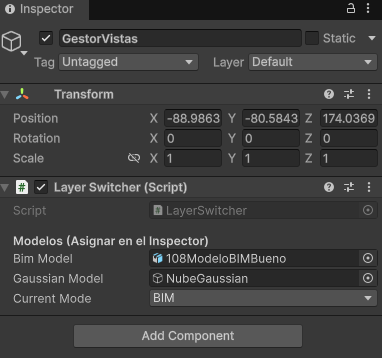
\includegraphics[width=0.7\linewidth]{include/images/figura5.1.png}
    \caption{Configuración del gestor de visualización en el motor de desarrollo}
    \label{fig:layer-switcher-unity}
\end{figure}


\section{Alineación Espacial de Modelos (Diseño vs Realidad)}

Para que el diagnóstico de desviaciones funcione correctamente, es indispensable que el modelo teórico de diseño y la reconstrucción tridimensional del edificio real compartan el mismo sistema de coordenadas globales. Dado que las capturas de la realidad suelen generarse con orígenes arbitrarios, se desarrolló un sistema matemático para automatizar la superposición precisa de ambos entornos.

El sistema emplea un algoritmo de emparejamiento basado en tres puntos de referencia homólogos definidos en ambos espacios:
\begin{itemize}
    \item \textbf{Punto 1 (Origen):} Define la traslación espacial exacta entre ambos mundos.
    \item \textbf{Punto 2 (Dirección Frontal):} Establece el vector de profundidad y la orientación cardinal.
    \item \textbf{Punto 3 (Dirección Superior):} Define el plano de apoyo y el vector de verticalidad.
\end{itemize}

Matemáticamente, el algoritmo calcula los vectores directores de orientación utilizando el producto vectorial entre las tres referencias establecidas. Con estos datos, el sistema determina la diferencia espacial de rotación existente y aplica de forma automática la transformación geométrica pertinente sobre el modelo escaneado. Esta corrección toma como referencia el punto de origen, logrando coincidir ambos modelos (Figura~\ref{fig:alineador}).

\begin{figure}[!htb]
    \centering
    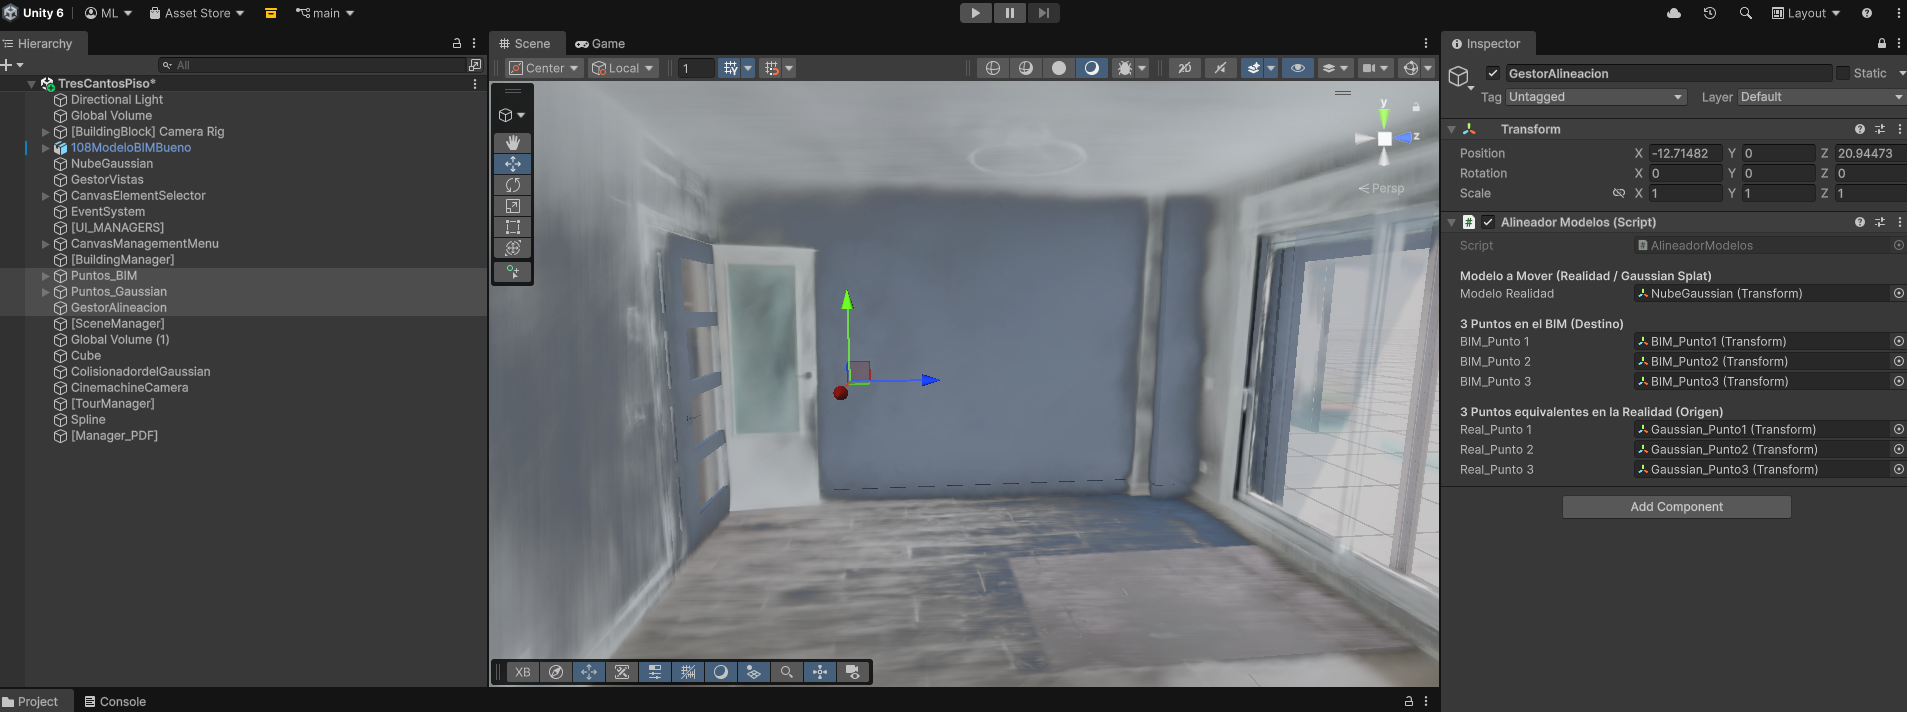
\includegraphics[width=0.8\linewidth]{include/images/figura5.7.png}
    \caption{Modelos alineados de forma automática}
    \label{fig:alineador}
\end{figure}

\section{Detección Automática de Colisiones}

Una de las fases más críticas en la coordinación de obras es la identificación de interferencias entre las instalaciones (conductos, tuberías) y los elementos estructurales (Figura~\ref{fig:MEP-struct}). Para automatizar este proceso, se implementó un módulo que evalúa las colisiones mediante la intersección de cajas delimitadoras tridimensionales.

Para evitar falsos positivos causados por roces superficiales (elementos que están en contacto válido pero no se atraviesan), el sistema realiza una reducción matemática de los límites de estas cajas antes de la evaluación. Si tras esta substracción los volúmenes se siguen intersecando, se confirma un conflicto estructural crítico.

Al detectar una interferencia, el sistema ejecuta tres acciones automatizadas:
\begin{enumerate}
    \item Instancia de manera procedural un marcador visual esférico en el centro exacto de la colisión, calculado a partir del promedio espacial de la superposición.
    \item Registra el impacto en el registro de datos global para su posterior volcado en el sistema de informes.
    \item Se comunica con el gestor de capas arquitectónicas enviando un conjunto de datos con las piezas involucradas. El sistema aísla automáticamente estos elementos, ocultando el resto del edificio para proporcionar al usuario una vista despejada del problema.
\end{enumerate}

\begin{figure}[!htb]
    \centering
    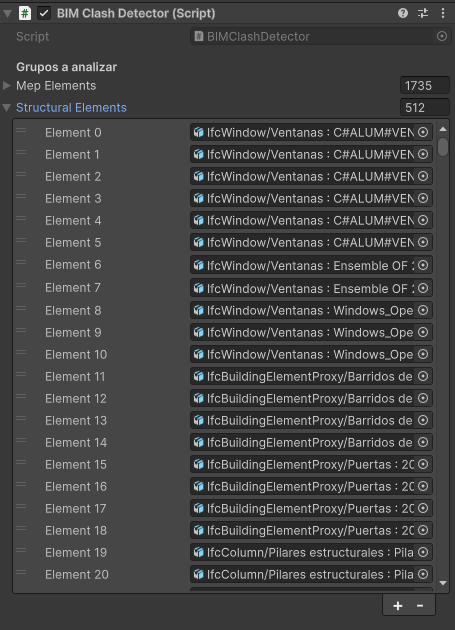
\includegraphics[width=0.8\linewidth]{include/images/figura5.8.png}
    \caption{Elementos divididos entre estructurales e instalaciones (MEP)}
    \label{fig:MEP-struct}
\end{figure}



\section{Sistema de Punteros e Interacción a Distancia}

En Realidad Virtual, el usuario necesita una referencia visual constante que indique la orientación de sus controladores para interactuar con interfaces o elementos distantes. Para lograrlo, se implementó un sistema de proyección que simula un "puntero láser".

El módulo calcula una línea poligonal continua en el espacio 3D. En cada iteración gráfica, el algoritmo toma la posición física de la mano del usuario como punto de origen y calcula un vector proyectado hacia adelante multiplicado por una constante de distancia. Para evitar que el rayo se comporte de forma errática al rotar la muñeca, se forzó el cálculo de los vértices sobre el espacio de coordenadas globales de la escena en lugar del local de la mano.

El láser resultante se renderizó con un grosor mínimo para simular precisión milimétrica, y se le aplicó un material puro sin cálculo de iluminación o sombras, garantizando que el haz de luz mantenga su visibilidad máxima sin importar las condiciones de oscuridad de la obra virtual. Como podemos observar en la Figura \ref{fig:rayvisual}, el rayo de cada controlador es distinto, al ser el izquierdo para seleccionar piezas es más grueso, y el derecho, al requerir un control más preciso es más fino.

\begin{figure}[!htb]
    \centering
    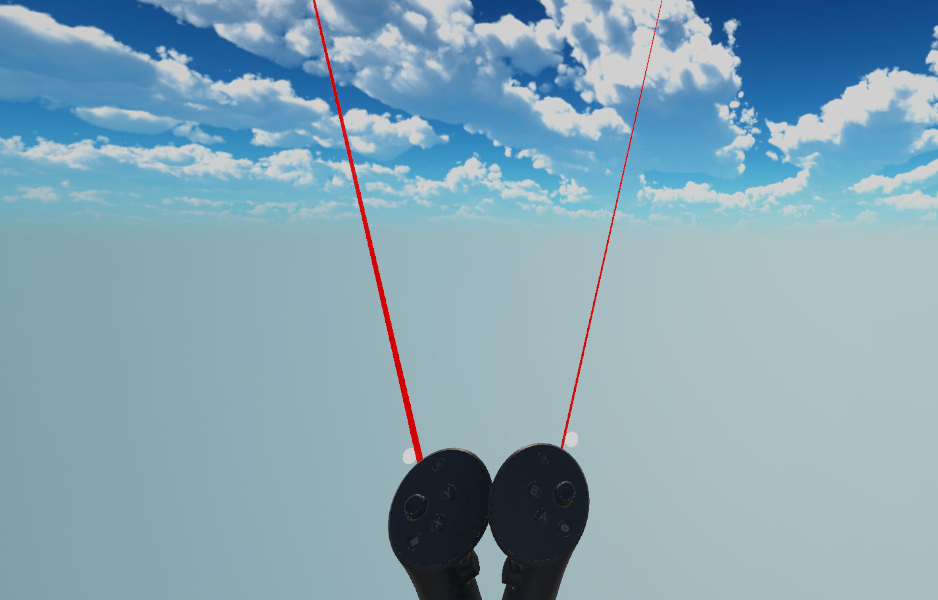
\includegraphics[width=0.8\linewidth]{include/images/controllerrayvisual.png}
    \caption{Raycast de cada controlador}
    \label{fig:rayvisual}
\end{figure}



\section{Inspección de Metadatos y Deconstrucción Selectiva}

El sistema permite apuntar a piezas individuales del diseño, extraer su información técnica (categoría, nombre de sistema, identificador) y visualizarla en un panel flotante (Figura \ref{fig:inspeccion}. Además, incluye la capacidad de ocultar el elemento seleccionado para visualizar el interior de las estructuras.

El algoritmo lanza un rayo físico invisible desde el mando que es filtrado mediante máscaras lógicas para asegurar que solo interactúa con geometría del edificio a inspeccionar. Al colisionar, se activa un retroalimentador visual que cambia el color de la pieza. El módulo de inspección fragmenta los datos del elemento objetivo para reconstruir una ficha técnica con formato legible.

El gestor de la interfaz calcula dinámicamente la posición del panel de información basándose en vectores espaciales. El panel se sitúa siempre a una distancia prudencial frente al usuario y se orienta hacia su línea de visión, garantizando la legibilidad (Figura~\ref{fig:ovr-controllers-unity}). El usuario puede ocultar la pieza inspeccionada mediante un comando directo, y el sistema memoriza estos elementos en una estructura de datos para permitir su restauración total mediante otro atajo en los controladores.

\begin{figure}[!htb]
    \centering
    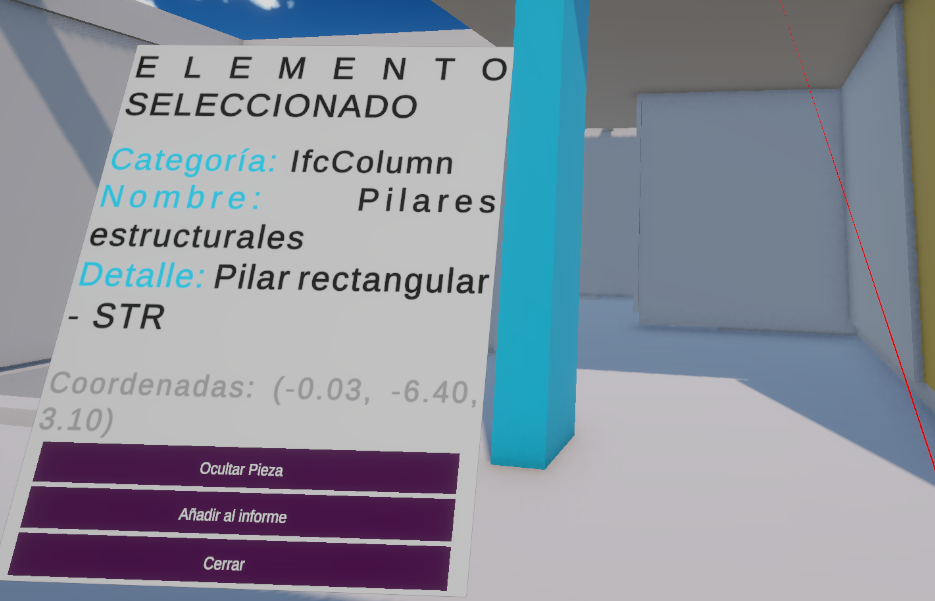
\includegraphics[width=0.8\linewidth]{include/images/inspeccion.png}
    \caption{Interfaz mostrada al inspeccionar una columna de manera individual}
    \label{fig:inspeccion}
\end{figure}

\begin{figure}[!htb]
    \centering
    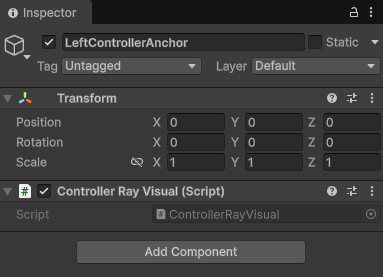
\includegraphics[width=0.5\linewidth]{include/images/figura5.2.png}
    \caption{Integración del sistema de control y selección de elementos en el entorno}
    \label{fig:ovr-controllers-unity}
\end{figure}

Para dotar a la herramienta de trazabilidad, el módulo de selección se integra con el motor documental. Al inspeccionar una pieza, el sistema evalúa si ya forma parte del registro de la auditoría. De no ser así, habilita una opción para registrar el elemento con sus coordenadas para su posterior exportación.


\subsection{Inteligencia Espacial y Prevención de Oclusiones}

Desplegar interfaces flotantes a una distancia estática presentaba un riesgo de oclusión severo: si el usuario inspeccionaba un elemento muy cercano a un muro, el panel atravesaba la pared física, imposibilitando su lectura. 

Para dotar a la interfaz de consciencia espacial, el sistema implementa un algoritmo de seguridad dinámico. Antes de hacer aparecer el menú, se proyecta un rayo desde los ojos del usuario hacia la coordenada ideal del panel, buscando intersecciones con elementos estructurales. Si se detecta un obstáculo, el algoritmo acorta matemáticamente el vector de distancia, reubicando la interfaz justo antes del punto de impacto. Se estableció además un límite de cercanía mínima absoluta para evitar problemas de enfoque ocular y fatiga visual.




\section{Herramienta de Medición Espacial Euclidiana}

Para evaluar discrepancias, el usuario cuenta con una "cinta métrica virtual" capaz de calcular distancias exactas entre cualquier par de puntos del espacio tridimensional a partir del modelo teórico. Visto en la Figura \ref{fig:informe-diseño}.

El sistema de medición opera mediante una máquina de estados controlada por las interacciones del operario:
\begin{enumerate}
    \item \textbf{Apuntado Inicial:} Se proyecta un láser secundario constante que indica el punto exacto de colisión física sobre las superficies, ignorando mediante un sistema de capas las interfaces flotantes para evitar mediciones erróneas.
    \item \textbf{Fijación del Primer Punto:} Al registrar la primera pulsación, se captura la coordenada tridimensional de origen. La cinta visual se ancla en este punto y se estira dinámicamente siguiendo la orientación de la mano del usuario.
    \item \textbf{Fijación del Segundo Punto:} Una segunda pulsación confirma la coordenada de destino. El algoritmo resuelve la distancia euclidiana exacta entre ambos puntos en el espacio. Esta medición se inyecta inmediatamente en la memoria de la sesión para el informe de auditoría.
    \item \textbf{Representación Visual:} Se genera dinámicamente un indicador de texto flotante que se sitúa en el punto medio geométrico exacto del segmento trazado, mostrando el valor métrico resultante.
\end{enumerate}




\section{Registro de Incidencias y Trazabilidad}

La aplicación provee un sistema para señalar problemas visuales manualmente y categorizarlos mediante marcadores espaciales (Grave, Leve o a Revisar, Figura \ref{fig:incidencia}), utilizando un flujo de trabajo optimizado para no interrumpir la inmersión.

Para no saturar la aplicación, en lugar de utilizar menús, la selección de la gravedad de la incidencia se realiza mediante la lectura del eje direccional del controlador derecho (arriba, izquierda o derecha), bloqueando el giro de la cámara hecho con el mismo. Al clavar la marca de incidencia en el entorno, se adjunta información textual. Para garantizar que estos marcadores sean siempre legibles desde cualquier ángulo de la sala, se implementó una rutina matemática de orientación continua (\textit{Billboarding}), la cual fuerza la rotación geométrica de las etiquetas para que encaren constantemente el vector de visión del usuario.

\begin{figure}[!htb]
    \centering
    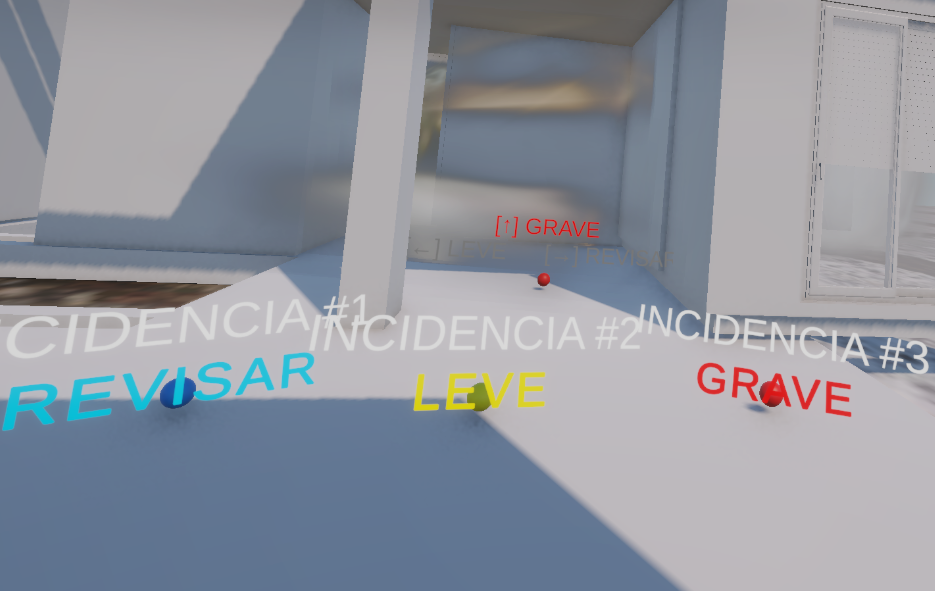
\includegraphics[width=0.8\linewidth]{include/images/incidencias.png}
    \caption{Niveles de incidencia posibles}
    \label{fig:incidencia}
\end{figure}


\section{Gestión y Filtrado de Tipologías Estructurales}

En la auditoría constructiva es habitual que más de un elemento superficial oculte sistemas críticos. Se desarrolló una herramienta de "deconstrucción" global que permite aislar o alterar la visibilidad de grupos enteros de elementos (como "Muros" o "Estructura") de forma masiva.

El sistema utiliza contenedores lógicos que agrupan listas de elementos tridimensionales según su tipología. Al arrancar, el sistema analiza el estado visible real del edificio. Posteriormente, permite ejecutar funciones de alternancia de visibilidad que iteran rápidamente sobre cientos de elementos para apagarlos o encenderlos simultáneamente. 

Dado que los controladores físicos tienen botones limitados, el mando sobre este sistema se delegó a una interfaz gráfica inmersiva, colocado cerca del punto de aparición del usuario. Cada categoría arquitectónica está vinculada a un botón bidimensional que envía la orden de visibilidad al contenedor correspondiente (Figura~\ref{fig:btn-capas-unity}).

\begin{figure}[!htb]
    \centering
    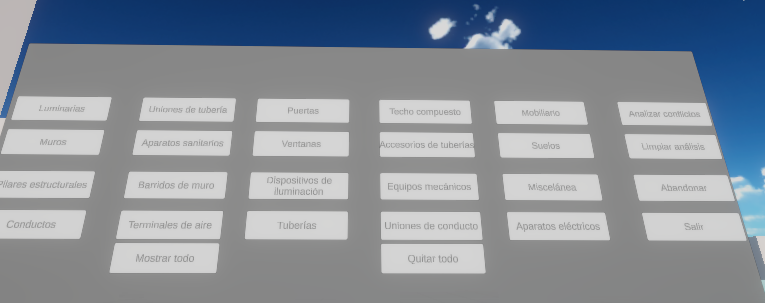
\includegraphics[width=0.8\linewidth]{include/images/figura5.3.png}
    \caption{Panel de gestión de capas estructurado en la interfaz inmersiva}
    \label{fig:btn-capas-unity}
\end{figure}



\section{Navegación e Interfaz Responsiva}

Para dotar a la aplicación de escalabilidad, se implementó un sistema de navegación entre diferentes modelos de edificios partiendo desde una sala central. El desafío técnico principal consistía en evitar que la manipulación de los menús activase accidentalmente las herramientas de auditoría.

Se implementó un sistema de exclusión basado en máscaras de colisión. El algoritmo detecta si el puntero láser está impactando sobre un elemento de la interfaz; de ser así, levanta una bandera lógica que desactiva temporalmente las herramientas métricas y de selección del entorno, enfocando las acciones del usuario exclusivamente hacia la navegación del menú.

Además, el láser visual se adaptó de forma dinámica: el haz de luz ahora calcula la distancia al primer objeto o sólido en su trayectoria y trunca su longitud en el punto de impacto, eliminando la ilusión óptica de un rayo que atraviesa las pantallas físicas. Los menús inmersivos reaccionan al tacto virtual modificando su color para que sean responsivas (Figura~\ref{fig:interfaz-menu}).

\begin{figure}[!htb]
    \centering
    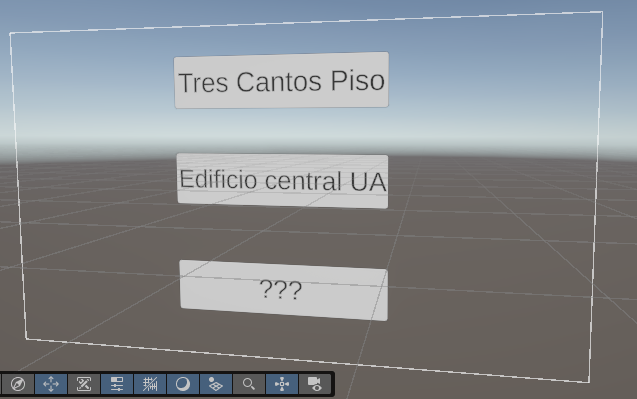
\includegraphics[width=0.8\linewidth]{include/images/figura5.4.png}
    \caption{Interfaz principal del menú y sistema de botones responsivos}
    \label{fig:interfaz-menu}
\end{figure}



\section{Interacciones y Prevención de Cinetosis}

Los cambios abruptos en el entorno virtual pueden romper la inmersión e inducir mareos. Para mitigarlo, se desarrolló un sistema de animaciones procedurales basadas en interpolación matemática. La aparición de menús u ocultación de elementos arquitectónicos no se produce de forma instantánea, sino alterando gradualmente su escala tridimensional. A esta transición se le aplicó una interpolación para que se sienta menos errático.

A la hora de interactuar con paneles virtuales, las herramientas estándar de Unity ofrecían una respuesta visual pobre. Se diseñó un módulo que reemplaza por completo el material de los botones al ser pulsados. Al realizar un intercambio de la propia textura en lugar de tintar la imagen, se respetan las sombras y brillos del entorno tridimensional, mejorando la respuesta táctil visual.

Para evitar mareos durante los tiempos de carga entre diferentes modelos arquitectónicos, las transiciones se delegaron a hilos de procesamiento en segundo plano, y se sincronizaron con un oscurecimiento progresivo de la visión del usuario. Esto garantiza que el seguimiento de los movimientos de la cabeza nunca se congele mientras el procesador prepara el nuevo entorno. Este oscurecimiento se logró creando un panel negro de gran tamaño delante de la cámara del usuario usuario (Figura~\ref{fig:camara}), que se hace visible progresivamente al cambiar de escena.

\subsection{Persistencia Local de Sesiones}
Se integró un sistema de almacenamiento ligero en la memoria del dispositivo que registra fechas y datos de inspección mediante cadenas de texto. Esta información se inyecta en la sala inicial, permitiendo al usuario llevar un control visual de las auditorías previas sin requerir complejas infraestructuras de bases de datos externas. Visto en la Figura \ref{fig:res-menu}.

\subsection{Desplazamiento Físico en Desniveles}
El desplazamiento por una maqueta implica subir o bajar escaleras. La simulación de gravedad estándar generaba caídas abruptas y micro-saltos al caminar rápidamente por un desnivel negativo. Para subsanarlo, el algoritmo aísla el cálculo de movimiento horizontal del vertical. Al detectar el borde de un escalón, el sistema realiza una presión vertical que actúa como un ancla magnética hacia la malla de las escaleras, forzando a descender adherido a la pendiente del peldaño y resultando en un tránsito fluido.




\section{Registro Documental y Generación de Informes}

Se implementó un sistema automático para documentar de manera visual y paramétrica las anomalías, el cual se divide en un subsistema de fotografía inmersiva y un motor de maquetación.

\subsection{Cámara Virtual Inmersiva}
Para capturar evidencias en obra, se desarrolló una herramienta que simula una cámara anclada a la mano del usuario, renderizando la perspectiva en una textura dinámica en tiempo real (Figura~\ref{fig:camara}). Al accionar el disparador, el algoritmo extrae la matriz de píxeles resultante, la codifica en un formato de imagen convencional y la almacena en el disco duro del visor. El proceso se acompaña de un efecto visual de destello sobre las lentes para confirmar la captura.

\begin{figure}[!htb]
    \centering
    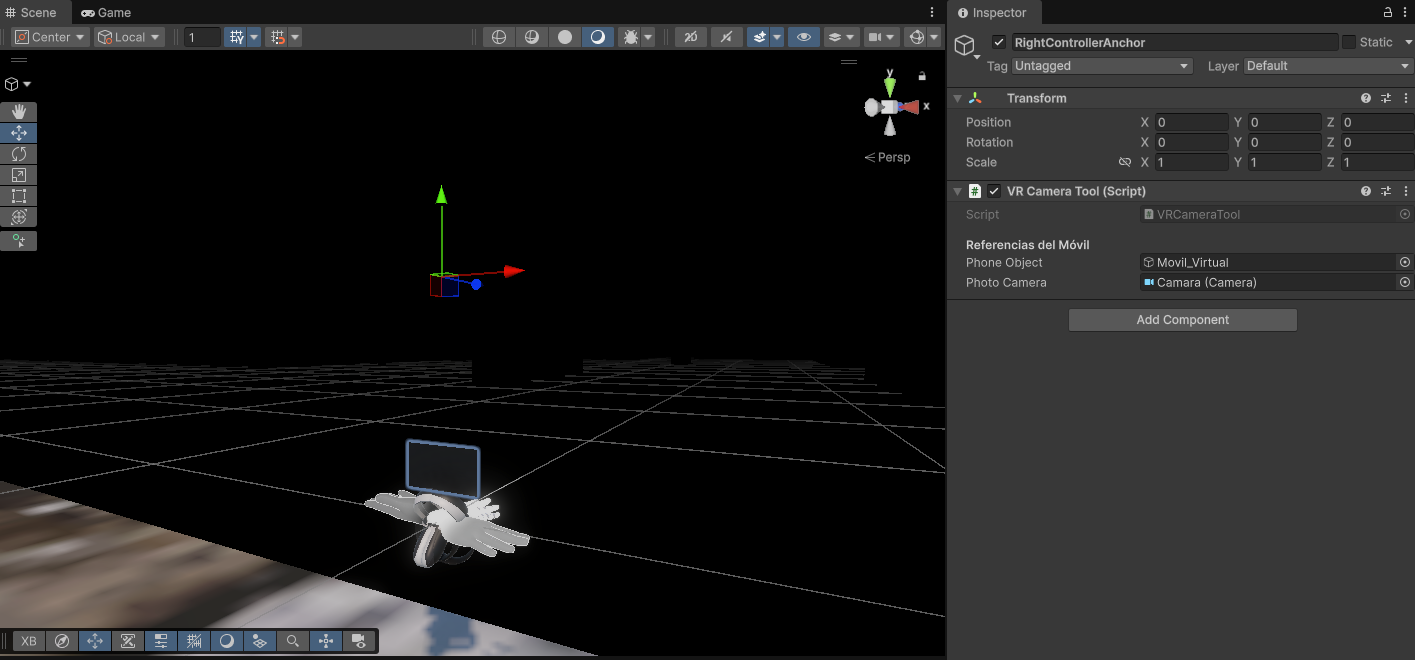
\includegraphics[width=0.8\linewidth]{include/images/figura5.10.png}
    \caption{Visualización inmersiva de la cámara para la captura de evidencias}
    \label{fig:camara}
\end{figure}

\subsection{Motor de Compilación de Datos}
La automatización del informe documental consiste en una arquitectura de memoria centralizada. Todas las herramientas de la aplicación operan independientemente, pero vuelcan sus hallazgos en estructuras de datos globales. Al solicitar la exportación, un motor basado en librerías de procesamiento de documentos organiza estos datos y diagrama en un archivo PDF.

Para una buena presentación, se encapsula lógicamente cada captura fotográfica junto a su texto descriptivo, forzando saltos de página inteligentes para evitar que queden huérfanos o separados. Tras compilar el archivo (Figura~\ref{fig:informe-diseño}), el sistema hace una limpieza de memoria, permitiendo realizar múltiples auditorías sucesivas sin reiniciar el programa.

\begin{figure}[!htb]
    \centering
    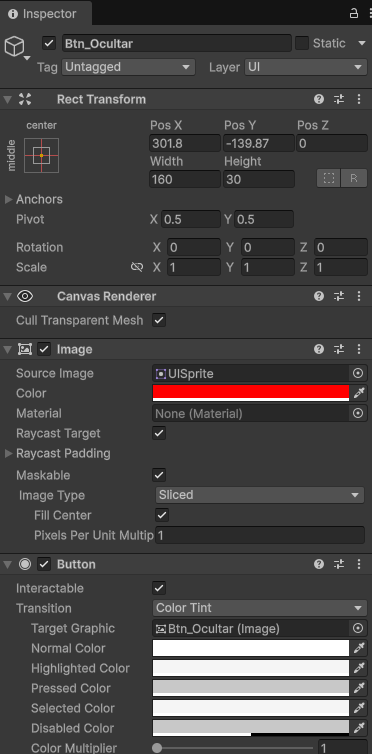
\includegraphics[width=0.8\linewidth]{include/images/figura5.5.png}
    \caption{Documento de auditoría final generado autónomamente por el sistema}
    \label{fig:informe-diseño}
\end{figure}






\section{Evaluación Volumétrica y Mapa de Calor Espacial}

Otra de las funciones de la aplicación para analizar es un escáner capaz de medir las diferencias entre la estructura real física y el modelo teórico en tiempo real. Esta herramienta tiñe los elementos del edificio teórico con un mapa de calor proyectado.

El desafío principal radicaba en que las digitalizaciones de la realidad carecen de volumen sólido, y procesar millones de partículas simultáneamente saturaría el procesador, volviendo la experiencia injugable. Para solucionarlo, el modelo volumétrico crudo se preprocesó mediante software especializado (CloudCompare) aplicando un submuestreo espacial, reduciendo considerablemente la densidad de puntos y aligerando el volumen de datos. Este modelo se exportó como documento de texto incluyendo todo el conjunto de puntos como coordenadas con el objetivo de optimizar el proceso y hacer posible esa comparación. A modo de prueba y validación, en la Figura \ref{fig:comparacion} se observa que los puntos cianes representan la versión simplificada del modelo con Gaussian Splat

\subsection{Algoritmo de Proximidad Topológica}
La herramienta de escáner ejecuta un cálculo de búsqueda espacial. Al interactuar con un muro teórico, el sistema analiza las coordenadas circundantes y evalúa la distancia hacia los puntos del modelo preprocesado.

Si el algoritmo confirma la existencia de masa física real dentro de un radio de tolerancia, verifica la validez de esa parte de la estructura.

\subsection{Clasificador de Desviaciones}
Esta evaluación se procesa a través de un sistema de clasificación gradual que analiza la magnitud del error detectado y altera en consecuencia la coloración de la superficie analizada:
\begin{itemize}
    \item \textbf{Verde (Perfecto):} Desviación ínfima. La obra física coincide íntegramente con el plano.
    \item \textbf{Amarillo (Aceptable):} Discrepancia leve pero asumible dentro de las tolerancias normales.
    \item \textbf{Naranja (Desviación Notable):} Error de ejecución evidente que requiere una revisión técnica.
    \item \textbf{Rojo (Fallo Crítico):} Ausencia total del elemento o desplazamiento que excede cualquier margen de seguridad permitido.
\end{itemize}

El resultado final es un diagnóstico inmersivo inmediato que, además de colorear la maqueta virtual (Figura~\ref{fig:comparacion}), registra cada comprobación para adjuntarla al informe global de la sesión.

\begin{figure}[!htb]
    \centering
    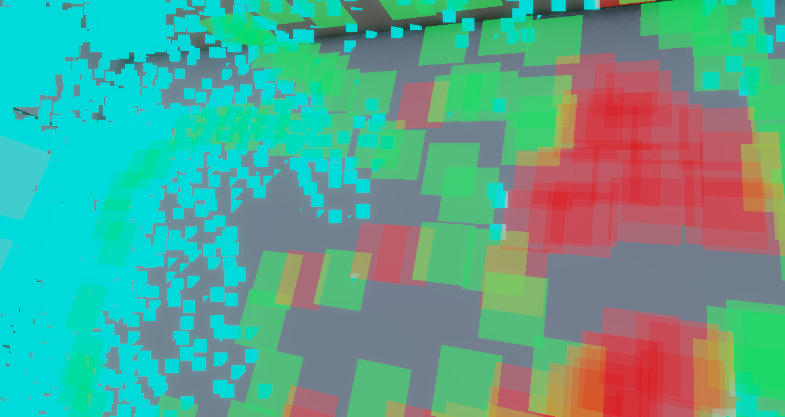
\includegraphics[width=0.8\linewidth]{include/images/figura5.6.png}
    \caption{Versión inicial del spray de mapa de calor con el modelo de puntos simplificado, inicialmente eran solo dos colores}
    \label{fig:comparacion}
\end{figure}		% Plantilla: Se muestran listados
\chapter{\label{resultados}Resultados}

Una vez finalizada la fase de desarrollo de la aplicación, en este capítulo se exponen los resultados finales obtenidos. Se detalla la solución inmersiva alcanzada mostrando las interfaces generadas, se evalúa su puesta en producción y métricas de rendimiento y se analizan los costes asociados frente a la planificación inicial. Finalmente, se realiza una reflexión académica sobre la relación del proyecto con el plan de estudios del Grado.

\section{Casos de Prueba y Modelos Arquitectónicos}
Para poner a prueba el software desarrollado, se ha probado de manera exitosa la aplicación a tres tipos de modelos arquitectónicos, demostrando una gran adaptabilidad a diferentes tipos de edificios.

\subsection{Apartamento Individual (Tres Cantos, Madrid)}
Este primer escenario representa una vivienda unifamiliar de un solo nivel. Ha sido el entorno principal empleado de forma continuada durante el ciclo de desarrollo de la aplicación, utilizándose como escena de pruebas en lugar de avanzar con los tres casos de forma simultánea. Resultó ser el modelo ideal para depurar las interacciones a corta distancia y calibrar el comportamiento de las herramientas inmersivas en espacios reducidos. Cabe destacar que, aunque el modelo de diseño teórico (BIM) comprende la vivienda en su totalidad, el acceso a la reconstrucción volumétrica de la realidad (\textit{Gaussian Splatting}) está limitado a una única habitación debido a la alta complejidad computacional y la falta de accesibilidad a dicho modelo. La proporción que tiene dicho modelo respecto a la totalidad del modelo teórico se puede apreciar en la Figura \ref{fig:trescantospiso}. 

\begin{figure}[!htb]
\centering
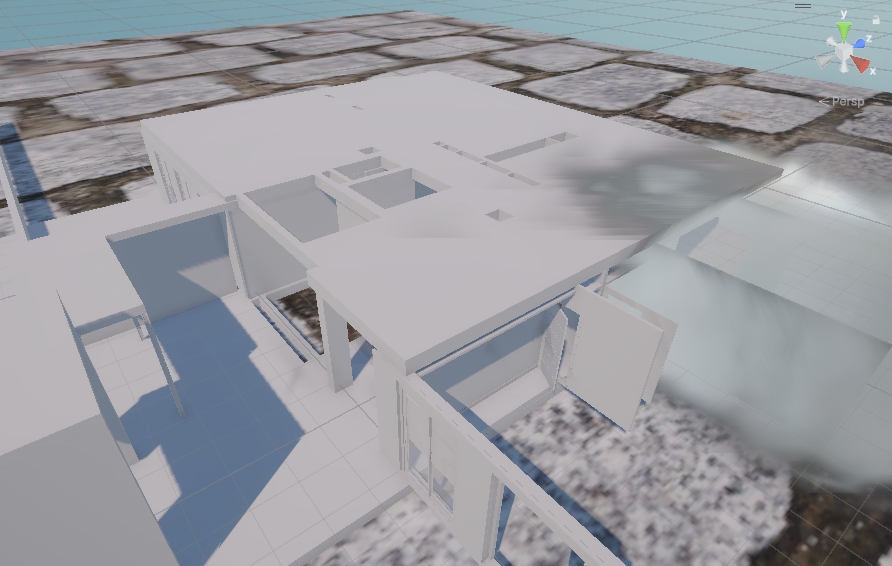
\includegraphics[width=0.8\linewidth]{include/images/trescantospiso.png}
\caption{Vista general del piso con el modelo de puntos apreciable en la parte derecha}
\label{fig:trescantospiso}
\end{figure}

\subsection{Aeródromo de la Universidad de Alicante}
Este modelo representa el entorno de la Antigua Torre de Control de las instalaciones universitarias. Al ser una estructura vertical y aislada que opera como edificio de oficinas y gestión, permitió testear los algoritmos de movimiento en desniveles (prevención de cinetosis en escaleras) y comprobar el rendimiento de los colisionadores con grandes ventanales y geometrías atípicas. Para este caso de estudio específico no se dispuso de una digitalización física de la realidad, operando exclusivamente sobre el entorno BIM para la validación de las lógicas de movimiento y físicas procedurales. En las Figuras \ref{fig:aerodromofull} y \ref{fig:aerodromo} se puede apreciar la diferencia del edificio en su totalidad con una versión descompuesta en solo puertas, ventanas, suelos y aparatos sanitarios.

\begin{figure}[!htb]
    \centering
    % ---- PRIMERA IMAGEN ----
    \begin{minipage}[b]{0.48\linewidth}
        \centering
        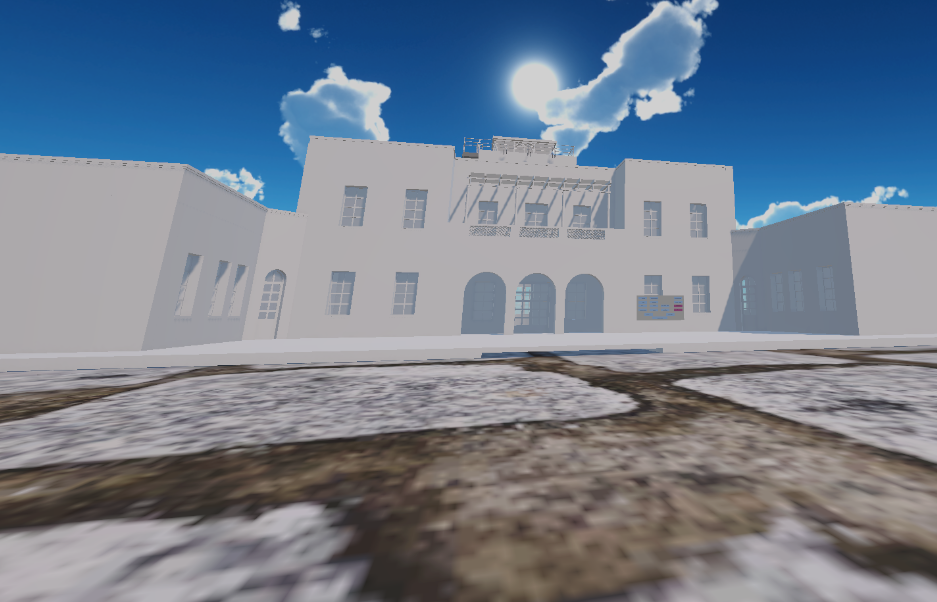
\includegraphics[width=\linewidth]{include/images/aerodromofull.png}
        \caption{Aeródromo completo en escena}
        \label{fig:aerodromofull}
    \end{minipage}
    \hfill
    % ---- SEGUNDA IMAGEN ----
    \begin{minipage}[b]{0.48\linewidth}
        \centering
        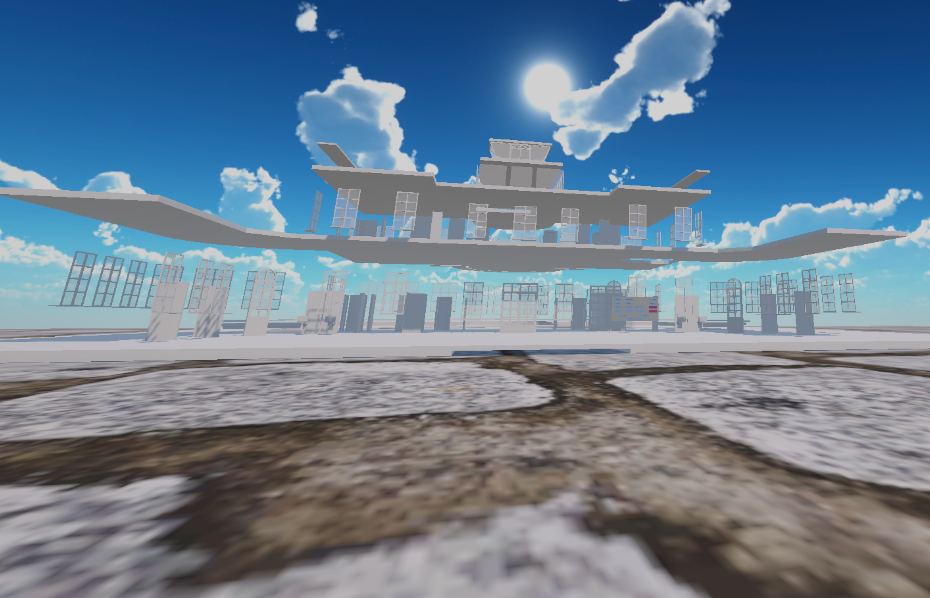
\includegraphics[width=\linewidth]{include/images/aerodromo.png}
        \caption{Aeródromo sin los muros}
        \label{fig:aerodromo}
    \end{minipage}
\end{figure}

Durante las pruebas en este modelo, se detectó que el tramo de escaleras superior tenía una pendiente excesivamente vertical, lo cual obstaculizaba el ascenso fluido del usuario mediante el sistema de movimiento continuo. Para solventar este problema de accesibilidad geométrica sin alterar la malla visual arquitectónica original, se superpuso un volumen de colisión invisible (\textit{Collider}) en forma de rampa con un ángulo de inclinación más suave. De esta forma la colisión del usuario se deslizará de manera natural hacia la planta superior, evitando bloqueos físicos o movimientos abruptos que pudieran romper la inmersión o inducir cinetosis. Visto en la Figura \ref{fig:escaleraauxiliar}.

\begin{figure}[!htb]
\centering
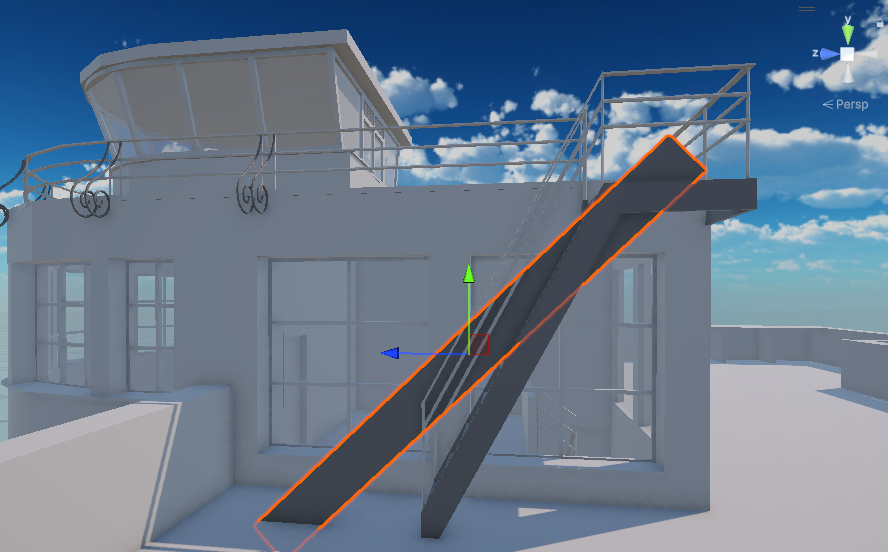
\includegraphics[width=0.8\linewidth]{include/images/escaleraauxiliar.png}
\caption{Malla de la "escalera" invisible}
\label{fig:escaleraauxiliar}
\end{figure}

\subsection{Complejo Residencial Nórdico (BIM4LCA)}
Por último, se implementó un modelo BIM altamente complejo y completo: un conjunto de apartamentos finlandés proporcionado por \textit{Nordic Sustainable Construction}. Este proyecto incluye una gran densidad poligonal y divisiones estructurales por plantas completas. Validar la aplicación en este macro-escenario sirvió como prueba para los algoritmos de optimización procedural de mallas y el gestor global de capas. 

Respecto a la representación de la obra física en este modelo, y como se anticipó en apartados anteriores de la memoria, se descartó la descarga o uso de un modelo \textit{Gaussian Splatting} de internet para evitar posibles infracciones de derechos de privacidad. Como solución técnica para probar el escáner espacial, mediante el software \textit{CloudCompare} se aisló exclusivamente la primera planta del edificio (Figura \ref{fig:thridmodel}) y se generó una nube de puntos convencional a partir del modelo teórico. Esta nube fue exportada directamente a un archivo de texto simplificado (\texttt{.txt}) para incluirlo al algoritmo de comparación de desviaciones. Como se puede observar en la Figura \ref{fig:wrongpiece}, para comprobar su funcionamiento despegó manualmente un muro del edificio.

\begin{figure}[!htb]
    \centering
    % ---- PRIMERA IMAGEN ----
    \begin{minipage}[b]{0.48\linewidth}
        \centering
        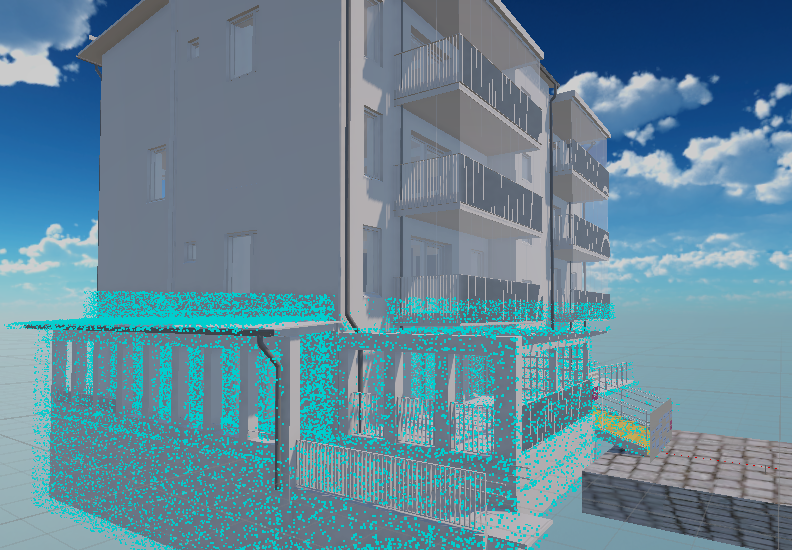
\includegraphics[width=\linewidth]{include/images/apartamentos.png}
        \caption{Edificio finlandés con modelos de puntos en el primer piso}
        \label{fig:thridmodel}
    \end{minipage}
    \hfill
    % ---- SEGUNDA IMAGEN ----
    \begin{minipage}[b]{0.48\linewidth}
        \centering
        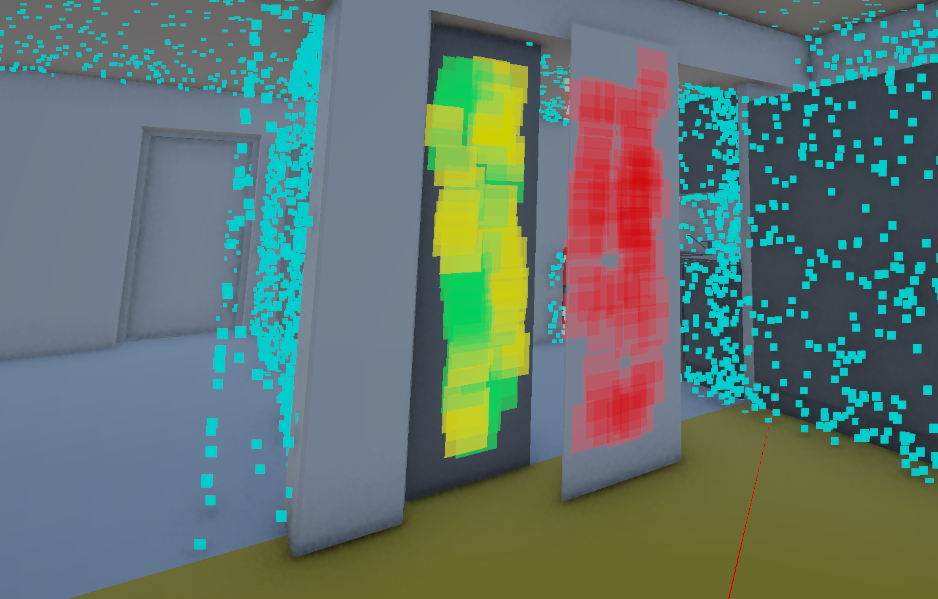
\includegraphics[width=\linewidth]{include/images/wrongpiece.png}
        \caption{Pieza desplazada marcado como rojo}
        \label{fig:wrongpiece}
    \end{minipage}
\end{figure}



\section{Descripción de la Solución Alcanzada}
El resultado principal de este proyecto es una aplicación funcional de Realidad Virtual orientada a la auditoría de obras y validación de entornos. El producto final se maneja en torno a varias interfaces y herramientas visuales operables de forma intuitiva, minimizando la carga cognitiva del operador.

\subsection{Interfaz Principal y Navegación}
Al iniciar la aplicación, el usuario accede a una sala o menú principal inmersivo. La interfaz ha sido diseñada priorizando la legibilidad espacial, previniendo el \textit{clipping} con el entorno y utilizando texturas reactivas al puntero láser. En este espacio, el operador puede consultar el registro persistente de fechas de las últimas inspecciones y seleccionar de forma fluida el entorno arquitectónico a auditar (Figura \ref{fig:res-menu}).

\begin{figure}[!htb]
\centering
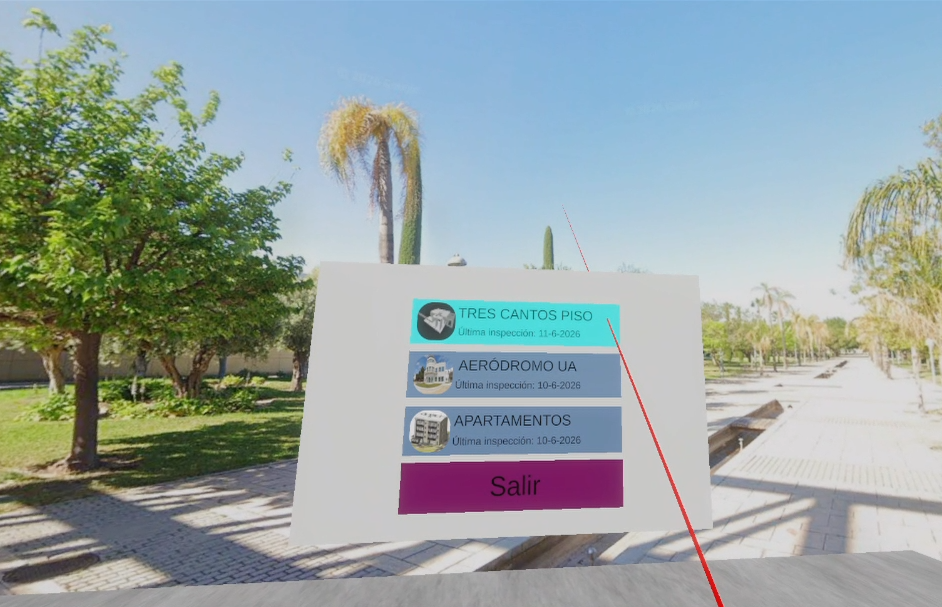
\includegraphics[width=0.8\linewidth]{include/images/figura6.1.png}
\caption{Captura del usuario en el menú principal viendo los paneles de selección de proyectos}
\label{fig:res-menu}
\end{figure}


En cada escena del edificio también se presentan botones para volver al menú principal o salir directamente de la propia aplicación.


\subsection{Herramientas de Auditoría Inmersiva}
El núcleo de la aplicación se manifiesta a través del conjunto de herramientas interactivas, las cuales devuelven resultados visuales y espaciales inmediatos al usuario:
\begin{itemize}
\item \textbf{Escáner de desviaciones (mapa de calor):} Se ha logrado proyectar visualmente la diferencia topológica entre el modelo teórico BIM y la captura de la realidad física. El resultado es un mapa de color paramétrico sobre las estructuras: verde para la coincidencia milimétrica y un degradado progresivo hacia el rojo para desviaciones estructurales críticas (Figura \ref{fig:res-escaner}).
\item \textbf{Cinta métrica y etiquetado espacial:} La herramienta genera cotas tridimensionales dinámicas que calculan distancias euclidianas exactas. Tanto estas mediciones como las etiquetas de incidencia (Graves, Leves o A Revisar) se mantienen siempre perfectamente legibles desde cualquier ángulo gracias a la técnica matemática de \textit{billboarding}.

\begin{figure}[!htb]
\centering
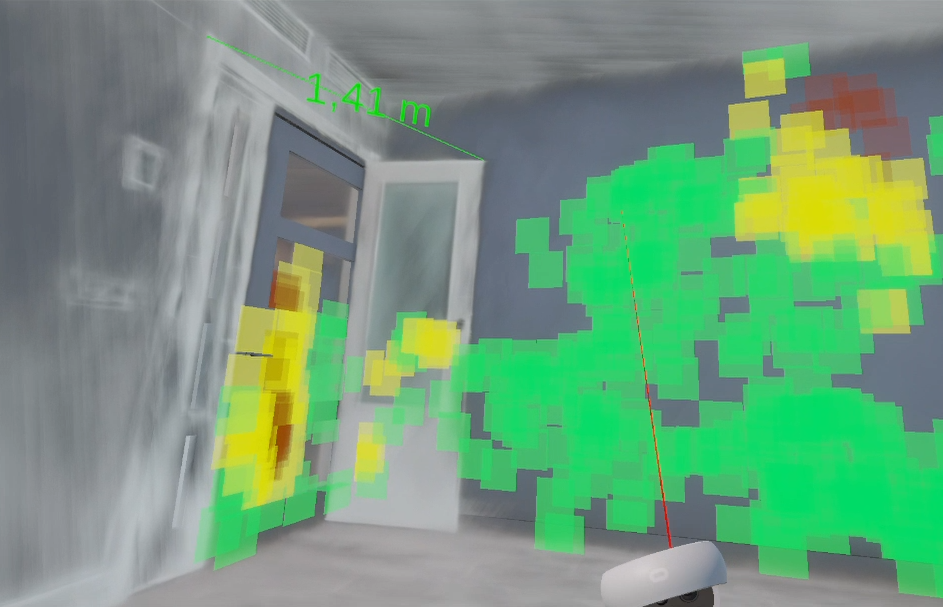
\includegraphics[width=0.8\linewidth]{include/images/figura6.2.png}
\caption{Captura desde los ojos del usuario usando el escáner de desviaciones y la cinta métrica}
\label{fig:res-escaner}
\end{figure}


\item \textbf{Gestión de capas y colisiones:} A través de un panel de control inmersivo adherido al controlador, el usuario puede aislar o deconstruir grupos estructurales masivos (Figura \ref{fig:aerodromo}). Asimismo, al ejecutar el detector de colisiones automatizado, la aplicación resalta visualmente mediante esferas las interferencias físicas entre instalaciones de conductos (MEP) y la arquitectura (Figura \ref{fig:conflicto}).
\end{itemize}

\begin{figure}[!htb]
\centering
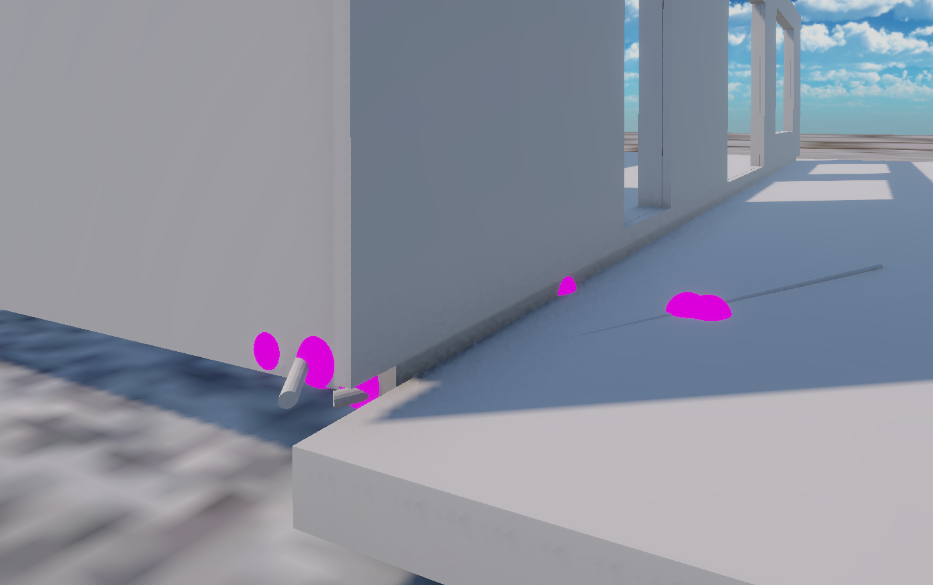
\includegraphics[width=0.8\linewidth]{include/images/conflicto.png}
\caption{Tuberías atravesando paredes y suelo en el apartamento unifamiliar}
\label{fig:conflicto}
\end{figure}


\subsection{Producto Documental: El Informe de Auditoría}
El resultado tangible y exportable del proyecto es un documento PDF generado directamente desde el entorno virtual. Tras emplear la cámara inmersiva y recopilar datos espaciales, el motor interno de maquetación compila un informe estructurado que consolida las fotografías con destellos de \textit{flash}, las incidencias categorizadas y las métricas de tolerancia de la obra. Este documento queda almacenado localmente. (Figura \ref{fig:res-pdf}).

\begin{figure}[!htb]
\centering
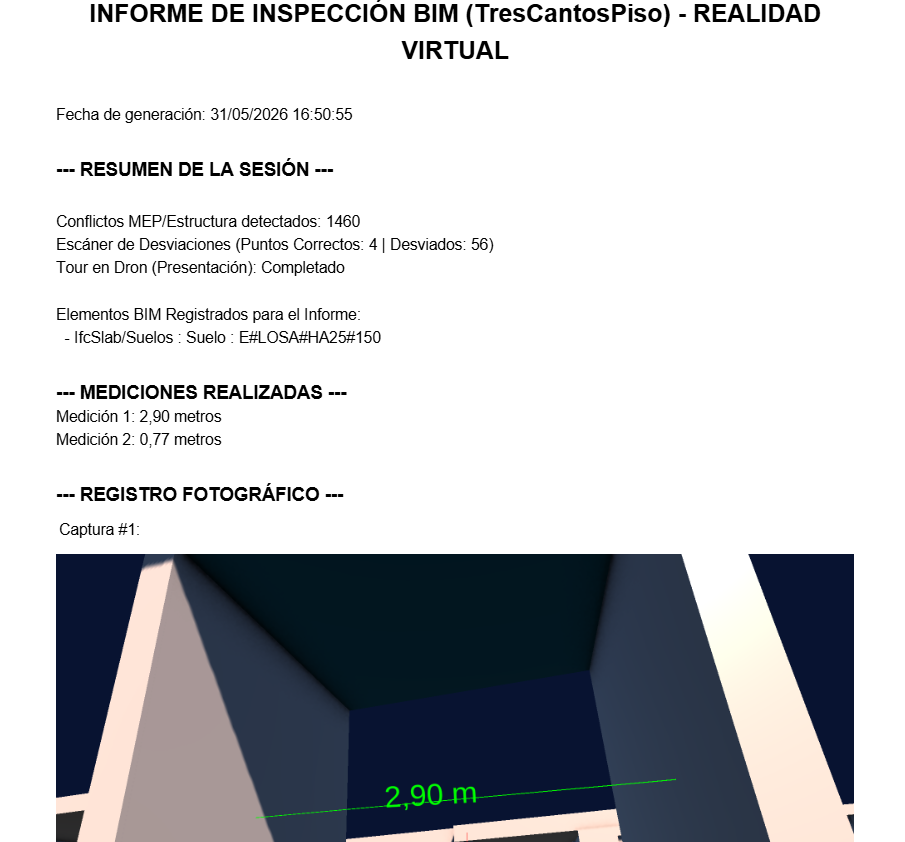
\includegraphics[width=0.8\linewidth]{include/images/figura6.3.png}
\caption{Captura de una de las páginas del PDF final generado por la aplicación (Registro fotográfico no visible)}
\label{fig:res-pdf}
\end{figure}

\section{Puesta en Producción, Métricas y Acceso}
Dada la especialización de la aplicación y el enorme peso de los modelos volumétricos, su puesta en producción excluye el despliegue masivo en tiendas de aplicaciones de consumo (\textit{App Stores}).

\begin{itemize}
\item Al trabajar con representaciones matemáticas densas como nubes de puntos pesadas y modelos BIM sin optimizar, la limitación de la memoria RAM unificada del visor (\textit{Standalone}) hace inviable la compilación en un paquete Android (\texttt{.apk}) convencional. Por ello, el modelo de despliegue recomendado consiste en generar una *Build* ejecutable nativa para entorno Windows. La aplicación se ejecuta aprovechando el cálculo de la GPU del ordenador y la experiencia visual se transmite al visor a través de cable link o por red local (\textit{Air Link}/\textit{Virtual Desktop}).
\item Al derivar la carga de procesamiento a la estación de trabajo local, la métrica de éxito más crítica, la tasa de fotogramas se mantiene alta y estable. Esto anula casi por completo la latencia visual, manteniendo la experiencia inmersiva cómoda para el usuario y minimizando el riesgo de cinetosis.
\item Las pruebas también demostraron que la arquitectura en PC permite almacenar y generar los informes PDF localmente a una velocidad superior. Además, la limpieza automática de los búferes de memoria tras la creación del documento permite ejecutar auditorías consecutivas sobre el modelo sin experimentar cierres por falta de memoria.
\end{itemize}

\section{Costes Finales y Comparativa de Planificación}
En términos de costes económicos, el desarrollo del software ha tenido un impacto financiero mínimo para la creación de este Trabajo de Fin de Grado. Se han empleado licencias académicas, repositorios gratuitos y herramientas de código abierto como el motor Unity, el procesador de nubes de puntos CloudCompare y las librerías dinámicas de C\# (iTextSharp). Los costes tangibles se limitan a la amortización técnica y energética del \textit{hardware} utilizado: el ordenador de escritorio para desarrollo y renderizado, y el visor Meta Quest 2 para el testing.

Desde el punto de vista temporal, el desarrollo se ha seguido en gran medida con la metodología de trabajo ágil (\textit{Kanban}) estipulada en las fases iniciales. Se registraron ligeras desviaciones temporales en el cronograma de investigación temprana, fundamentalmente vinculadas a incompatibilidades iniciales al renderizar el \textit{Gaussian Splatting} en Unity, así como a la adaptación a la lógica asíncrona de C\#. No obstante, estas demoras se mitigaron utilizando eficazmente los márgenes de seguridad proyectados en el cronograma, logrando desplegar un producto integral y funcional dentro del plazo académico.

\section{Viabilidad comercial}

En relación a la viabilidad comercial y vías de monetización post-académica, la aplicación desarrollada se orientaría a un modelo \textit{\gls{saas}} con suscripciones mensuales o anuales escaladas según el volumen de proyectos de la constructora.  

Los costes futuros asociados al despliegue se centrarían principalmente en el mantenimiento de la infraestructura de servidores en la nube para el almacenamiento de las nubes de puntos pesadas y el tráfico de datos de los informes. Teniendo en cuenta que el coste de reparar un fallo estructural menor detectado de forma tardía en una obra real suele superar con creces el precio de una licencia de software anual, el retorno de la inversión (ROI) para las empresas del sector resulta competitivo, consolidando la viabilidad comercial a largo plazo de esta solución tecnológica.

















\subsection{Experimento FPS vs Puntos}

Para medir el límite computacional de la aplicación durante su ejecución, se realizaron mediciones de FPS a la escena principal como prueba. Consistió en evaluar la tasa de fotogramas ante distintas cargas de densidad del modelo \textit{Gaussian Splatting}, aplicando simplificaciones sobre ésta (842.344 puntos). 

Los resultados de las cuatro pruebas realizadas se detallan en el Cuadro~\ref{tab:fps_splatting}:

\begin{table}[!htb]
    \centering
    \caption{Rendimiento de la aplicación según la densidad volumétrica (\textit{Gaussian Splatting})}
    \label{tab:fps_splatting}
    \begin{tabular}{lccc}
        \toprule
        \textbf{Categoría / Calidad} & \textbf{Porcentaje} & \textbf{Nº de Puntos} & \textbf{Tasa media (FPS)} \\
        \midrule
        Calidad Original (Nivel 1) & 100\,\% & 842.344 & 15 \\
        Simplificación Leve (Nivel 2) & 75\,\% & 631.758 & 18 \\
        Simplificación Media (Nivel 3) & 50\,\% & 421.172 & 18 \\
        Simplificación Alta (Nivel 4) & 25\,\% & 210.586 & 23 \\
        \bottomrule
    \end{tabular}
\end{table}

El análisis de los datos del experimento permite extraer dos conclusiones fundamentales sobre la arquitectura del sistema:

\begin{enumerate}
    \item \textbf{Estancamiento del rendimiento:} Al reducir la cantidad de puntos un 25\,\% (Nivel 2), el visor experimenta una leve mejora de 3 FPS. Sin embargo, al simplificar la muestra hasta la mitad exacta (Nivel 3), se mantiene estancado en los mismos 18 FPS. Este comportamiento demuestra que, una vez reducido el número de puntos, el problema ya no es la cantidad de datos, sino el esfuerzo que debe realizar la tarjeta gráfica para dibujar y superponer los elementos semitransparentes en la pantalla.
    \item \textbf{Inviabilidad autónoma (.apk):} Incluso aplicando una simplificación extrema que elimina tres cuartas partes del modelo (Nivel 4), el hardware del ordenador apenas logra alcanzar los 23 FPS, situándose muy por debajo del umbral mínimo de los 72 FPS exigidos por la industria para prevenir la cinetosis en Realidad Virtual.
\end{enumerate}

Estas mediciones apoyan la decisión de que la ejecución de digitalizaciones complejas mediante \textit{Gaussian Splatting} en visores requiere de forma obligatoria derivar la carga gráfica a un ordenador externo mediante transmisión.




































\section{Vinculación Académica sobre el Grado}
El diseño de este proyecto representa la culminación práctica de múltiples competencias, lógicas y metodologías asimiladas a lo largo de la titulación en Ingeniería Multimedia. El producto final de esta aplicación es resultado de aplicar conocimientos provenientes de las siguientes áreas:

\begin{itemize}
\item \textbf{Realidad Virtual (21040):} Durante este curso 2025-2026 en el grado se ha impartido esta asignatura, y ha sido una de las más relacionadas con el trabajo, otorgando experiencia similar en un motor diferente, Unreal Engine. Se han puesto en práctica fundamentos tales como el trazado de rayos (\textit{Raycasting}), interacción de 6DoF con mandos, y la prevención de la cinetosis a través de la interfaz.
\item \textbf{Usabilidad y Accesibilidad (21013):} Las directrices de estas materias han sido imprescindibles para el diseño de paneles de interfaces de usuario inmersivas, traduciendo elementos convencionales 2D (\textit{Canvas}) a espacios euclidianos interactivos. Se priorizó el contraste en los menús y la accesibilidad para usuarios que pudiesen padecer fatiga ocular en inmersiones prolongadas.
\item \textbf{Estructura de Datos y Algoritmia (21014):} Ha sido fundamental para la lógica del código; empleando diccionarios, *HashSets* paramétricos, listas dinámicas y árboles para aislar y procesar de manera concurrente los miles de componentes y metadatos que conforman la topología BIM.
\item \textbf{Fundamentos de videojuegos (21027) y Análisis y Especificación de Sistemas Multimedia (21017):} Proveyeron la base del flujo de trabajo: adopción de ciclos de trabajo de la metodología ágil, el diseño del modelo documental de arquitectura de software, el dominio de los repositorios de control de versiones (Git) y la correcta especificación funcional ante requerimientos cambiantes y desafíos técnicos inesperados.
\item \textbf{Dispositivos e Infraestructuras para Sistemas Multimedia (21021):} Respecto a la parte teórica contribuyó a la investigación del estado del arte, proporcionando información sobre los distintos tipos de pantalla (por ejemplo LCD), procesadores integrados en el propio equipo informático (SoC), o conceptos como IoT.
\item \textbf{Administración de empresas (21004):} Ha resultado útil para la elaboración del estudio de viabilidad, demostrando que, previo a cualquier desarrollo técnico, llega a ser prácticamente crucial realizar un estudio de mercado. La elaboración del modelo \textit{Lean Canvas}, hecho durante la materia ha permitido analizar de forma estructurada la viabilidad comercial de llevar a cabo este proyecto.
\end{itemize}		% Plantilla: Se muestran gráficas
\chapter{Conclusiones y Trabajo Futuro\label{conclusiones}}

En este último capítulo se recopilan las conclusiones finales extraídas a lo largo del diseño, desarrollo e implementación de la plataforma inmersiva de auditoría arquitectónica. Se evalúa el grado de cumplimiento de los objetivos establecidos al inicio del proyecto, se analiza el impacto potencial del sistema en el sector de la edificación y, por último, se proponen las líneas de trabajo futuro para la evolución del software más allá del marco de este Trabajo de Fin de Grado.

\section{Consecución de Objetivos}
Tras finalizar el desarrollo de la herramienta y la realización de las pruebas en el motor gráfico, se puede afirmar que los objetivos propuestos originalmente se han alcanzado en su mayoría. El propósito principal de reducir la brecha entre el diseño teórico de un edificio (BIM) y su ejecución real en obra se ha resuelto con éxito mediante la fusión de tecnologías XR y reconstrucción volumétrica tridimensional (\textit{Gaussian Splatting}).

Específicamente, se ha consolidado un entorno inmersivo estable y fluido capaz de procesar nubes de puntos complejas previamente optimizadas mediante técnicas de submuestreo espacial y \gls{sor}. Las herramientas operacionales como el escáner de desviaciones mediante mapas de calor, la cinta métrica tridimensional, el detector automatizado de colisiones estructurales con aislamiento de componentes y el módulo de captura fotográfica se encuentran plenamente integradas y operativas. La aplicación no solo actúa como un visualizador, sino que cumple con el requisito de unificar todos los datos en un motor procedural que compila de forma automática informes documentales en formato PDF listos para su uso profesional.

\section{Repercusión en el Entorno Destino}
La introducción de soluciones de Realidad Virtual orientadas al flujo de trabajo de construcción influencia positivamente a la comunidad y la industria de la construcción:
\begin{itemize}
    \item \textbf{Reducción de costes por errores de ejecución:} En la gestión de obras tradicional, un error geométrico o una interferencia entre una tubería MEP y un elemento estructural que no se detecta a tiempo se traduce en demoras masivas y sobrecostes económicos de demolición y reconstrucción. Esta herramienta permite anticipar dichos conflictos en fases tempranas mediante una inspección visual intuitiva a escala real 1:1.
    \item \textbf{Democratización del acceso a datos técnicos:} Tradicionalmente, la interpretación de nubes de puntos densas o modelos de coordinación requería software de escritorio complejo y personal altamente cualificado. Al trasladar esta información a una experiencia inmersiva natural, cualquier agente involucrado (promotores, arquitectos, contratistas o clientes finales) puede comprender las medidas y el estado real de la obra sin necesidad de formación técnica avanzada.
    \item \textbf{Optimización del flujo de información:} La capacidad de generar informes técnicos unificados directamente desde el visor VR acorta los tiempos de comunicación entre el personal de campo y la oficina técnica, acelerando la toma de decisiones y el control de calidad.
\end{itemize}

\section{Limitaciones y Líneas de Trabajo Futuro}
A pesar de haber alcanzado un producto mínimo viable completamente funcional que cumple con los objetivos principales del proyecto, el proceso de desarrollo e investigación ha demostrado ciertas limitaciones técnicas y ventanas de oportunidad. Debido a las restricciones temporales inherentes a un Trabajo de Fin de Grado y a la complejidad de las tecnologías XR, las siguientes funcionalidades no pudieron ser integradas en la versión actual y se proponen como futuras líneas de investigación y desarrollo:

\begin{itemize}
    \item \textbf{Integración de Realidad Aumentada (AR):} Aunque la aplicación resuelve de manera óptima la inspección inmersiva en entornos virtuales (VR), quedó fuera del alcance la implementación de un módulo de Realidad Aumentada. Esta funcionalidad habría permitido superponer el modelo digital BIM directamente sobre el terreno físico real de la obra utilizando técnicas de geolocalización y visión artificial, lo cual potenciaría las capacidades de auditoría sobre el propio emplazamiento.
    \item \textbf{Automatización de la importación:} Actualmente, la incorporación de un nuevo edificio requiere una serie de procesos de configuración manual dentro del editor de Unity (organización jerárquica de capas, preparación de los colisionadores y ajuste de variables del escáner). Una línea futura clave consiste en el desarrollo de un algoritmo en tiempo de ejecución que automatice por completo la creación de la escena con solo depositar el archivo del modelo, eliminando la dependencia del entorno de desarrollo.
    \item \textbf{Entorno colaborativo multiusuario:} La arquitectura actual de la aplicación está diseñada para sesiones individuales de un único usuario. La integración de un sistema de red y sincronización (como \textit{Unity Netcode} o \textit{Photon Fusion}) permitiría habilitar sesiones multiusuario concurrentes, facilitando que múltiples inspectores, arquitectos y directores de obra interactúen simultáneamente en la misma maqueta virtual para discutir las incidencias de forma remota.
    \item \textbf{Fidelidad y estética de la Interfaz de Usuario (UI):} Los paneles y menús desarrollados cumplen estrictamente con los requisitos funcionales de diseño responsivo, técnicas anti-clipping y prevención de fatiga visual. No obstante, a nivel estético presentan un acabado básico e industrial. Un desarrollo posterior enfocado en el pulido estético permitiría generar interfaces más detalladas, integrando elementos interactivos avanzados y menús que eleven la calidad visual del producto.
    \item \textbf{Sincronización en la nube y conectividad:} El motor de informes actual exporta los documentos PDF y las capturas fotográficas guardándolos de forma local en el almacenamiento persistente del visor Meta Quest. Una mejora a considerar sería la implementación de un servicio de sincronización automática con repositorios en la nube (como \textit{Firebase} o servidores BIM corporativos), permitiendo que los informes de auditoría estén disponibles de manera instantánea en las oficinas tras concluir la inspección.
    \item \textbf{Recorrido virtual guiado (tour automatizado):} Inicialmente se contempló la inclusión de un sistema de vuelo cinemático "sobre raíles" para presentar el modelo BIM de forma automática. Sin embargo, esta funcionalidad fue descartada durante la fase de desarrollo debido a que forzar el desplazamiento y la rotación de la cámara generaba cinetosis con excesiva facilidad. Sumado a los conflictos técnicos que presentaba forzar ese movimiento de la cámara y que se trataba de una característica secundaria respecto a las herramientas centrales de auditoría, se decidió prescindir de ella para priorizar la estabilidad del entorno.
\end{itemize}

%\section{Dificultad Global del Proyecto e Impresiones Personales}
%El desarrollo de este Trabajo de Fin de Grado ha supuesto dentro del grado de Ingeniería Multimedia un desafío de gran envergadura. La principal dificultad técnica no solo fue la programación aislada de las mecánicas de interacción, sino en la convergencia de estándares industriales dispares (formatos IFC provenientes de la arquitectura frente a mallas poligonales optimizadas para videojuegos) y en las severas restricciones de rendimiento gráfico que imponen los visores de Realidad Virtual autónomos (\textit{Standalone}). 

%Equilibrar la balanza entre la alta fidelidad visual que exige una auditoría de obra y el mantenimiento de una tasa de fotogramas por segundo (FPS) elevada para garantizar el confort del usuario supuso un exhaustivo proceso de optimización arquitectónica. Fue necesario abordar problemas complejos de computación gráfica, tales como la evasión de cuellos de botella en la memoria RAM mediante corrutinas asíncronas para la asignación procedimental de colisionadores, la simplificación del cálculo de distancias euclidianas eludiendo raíces cuadradas pesadas en la CPU y la reconfiguración del búfer gráfico para el renderizado estable de mapas de calor.

%A nivel personal, este proyecto ha constituido una de las experiencias de aprendizaje más enriquecedoras de toda la etapa universitaria. Ha demandado una actitud proactiva para investigar tecnologías emergentes en constante evolución (como el \textit{Gaussian Splatting}) y ha forzado la aplicación transversal de disciplinas del grado, desde la algoritmia pura y las estructuras de datos hasta el diseño de interfaces inmersivos. La satisfacción de transformar líneas de código abstractas en una herramienta tangible y de alta utilidad industrial reafirma la vocación ingenieril del autor.	% Plantilla: Se muestran matemáticas

%%%%
% CONTENIDO. BIBLIOGRAFÍA.
%%%%
\nocite{*} %incluye TODOS los documentos de la base de datos bibliográfica sean o no citados en el texto
\bibliography{bibliografia/bibliografia} % Archivo que contiene la bibliografía
\bibliographystyle{apacite}

% Incluye el listado de acrónimos utilizados en el trabajo. 
\printglossary[style=modsuper,typ%\input{include/estiloscodigoprogramacion.tex}
e=\acronymtype,title={Lista de Acrónimos y Abreviaturas}]
% Añade el resto de acrónimos si así se desea. Si no elimina el comando siguiente
\glsaddallunused 


\end{document}
